% **************************************************************************************************************
% A Classic Thesis Style
% An Homage to The Elements of Typographic Style
%
% Copyright (C) 2018 André Miede and Ivo Pletikosić
%
% If you like the style then I would appreciate a postcard. My address
% can be found in the file ClassicThesis.pdf. A collection of the
% postcards I received so far is available online at
% http://postcards.miede.de
%
% License:
% This program is free software; you can redistribute it and/or modify
% it under the terms of the GNU General Public License as published by
% the Free Software Foundation; either version 2 of the License, or
% (at your option) any later version.
%
% This program is distributed in the hope that it will be useful,
% but WITHOUT ANY WARRANTY; without even the implied warranty of
% MERCHANTABILITY or FITNESS FOR A PARTICULAR PURPOSE.  See the
% GNU General Public License for more details.
%
% You should have received a copy of the GNU General Public License
% along with this program; see the file COPYING.  If not, write to
% the Free Software Foundation, Inc., 59 Temple Place - Suite 330,
% Boston, MA 02111-1307, USA.
%
% PLEASE SEE ALSO THE AUTHORS' NOTE REGARDING THIS LICENSE
% IN THE DOCUMENTATION (ClassicThesis.pdf --> Chapter 1 / Chapter01.tex)
% **************************************************************************************************************
\RequirePackage{silence} % :-\
    \WarningFilter{scrreprt}{Usage of package `titlesec'}
    %\WarningFilter{scrreprt}{Activating an ugly workaround}
    \WarningFilter{titlesec}{Non standard sectioning command detected}
\documentclass[ twoside,openright,titlepage,numbers=noenddot,%1headlines,
                headinclude,footinclude,cleardoublepage=empty,abstract=on,
                BCOR=5mm,paper=a4,fontsize=11pt
                ]{scrreprt}

%********************************************************************
% Note: Make all your adjustments in here
%*******************************************************
% ****************************************************************************************************
% classicthesis-config.tex
% formerly known as loadpackages.sty, classicthesis-ldpkg.sty, and classicthesis-preamble.sty
% Use it at the beginning of your ClassicThesis.tex, or as a LaTeX Preamble
% in your ClassicThesis.{tex,lyx} with % ****************************************************************************************************
% classicthesis-config.tex
% formerly known as loadpackages.sty, classicthesis-ldpkg.sty, and classicthesis-preamble.sty
% Use it at the beginning of your ClassicThesis.tex, or as a LaTeX Preamble
% in your ClassicThesis.{tex,lyx} with % ****************************************************************************************************
% classicthesis-config.tex
% formerly known as loadpackages.sty, classicthesis-ldpkg.sty, and classicthesis-preamble.sty
% Use it at the beginning of your ClassicThesis.tex, or as a LaTeX Preamble
% in your ClassicThesis.{tex,lyx} with \input{classicthesis-config}
% ****************************************************************************************************
% If you like the classicthesis, then I would appreciate a postcard.
% My address can be found in the file ClassicThesis.pdf. A collection
% of the postcards I received so far is available online at
% http://postcards.miede.de
% ****************************************************************************************************


% ****************************************************************************************************
% 0. Set the encoding of your files. UTF-8 is the only sensible encoding nowadays. If you can't read
% äöüßáéçèê∂åëæƒÏ€ then change the encoding setting in your editor, not the line below. If your editor
% does not support utf8 use another editor!
% ****************************************************************************************************
\PassOptionsToPackage{utf8}{inputenc}
  \usepackage{inputenc}

\PassOptionsToPackage{T1}{fontenc} % T2A for cyrillics
  \usepackage{fontenc}


% ****************************************************************************************************
% 1. Configure classicthesis for your needs here, e.g., remove "drafting" below
% in order to deactivate the time-stamp on the pages
% (see ClassicThesis.pdf for more information):
% ****************************************************************************************************
\PassOptionsToPackage{
  drafting=true,    % print version information on the bottom of the pages
  tocaligned=false, % the left column of the toc will be aligned (no indentation)
  dottedtoc=false,  % page numbers in ToC flushed right
  eulerchapternumbers=true, % use AMS Euler for chapter font (otherwise Palatino)
  linedheaders=false,       % chaper headers will have line above and beneath
  floatperchapter=true,     % numbering per chapter for all floats (i.e., Figure 1.1)
  eulermath=false,  % use awesome Euler fonts for mathematical formulae (only with pdfLaTeX)
  beramono=true,    % toggle a nice monospaced font (w/ bold)
  palatino=true,    % deactivate standard font for loading another one, see the last section at the end of this file for suggestions
  style=classicthesis % classicthesis, arsclassica
}{classicthesis}


% ****************************************************************************************************
% 2. Personal data and user ad-hoc commands (insert your own data here)
% ****************************************************************************************************
\newcommand{\myTitle}{A Classic Thesis Style\xspace}
\newcommand{\mySubtitle}{An Homage to The Elements of Typographic Style\xspace}
\newcommand{\myDegree}{Doktor-Ingenieur (Dr.-Ing.)\xspace}
\newcommand{\myName}{André Miede \& Ivo Pletikosić\xspace}
\newcommand{\myProf}{Put name here\xspace}
\newcommand{\myOtherProf}{Put name here\xspace}
\newcommand{\mySupervisor}{Put name here\xspace}
\newcommand{\myFaculty}{Put data here\xspace}
\newcommand{\myDepartment}{Put data here\xspace}
\newcommand{\myUni}{Put data here\xspace}
\newcommand{\myLocation}{Saarbrücken\xspace}
\newcommand{\myTime}{June 2018\xspace}
\newcommand{\myVersion}{\classicthesis}

% ********************************************************************
% Setup, finetuning, and useful commands
% ********************************************************************
\providecommand{\mLyX}{L\kern-.1667em\lower.25em\hbox{Y}\kern-.125emX\@}
\newcommand{\ie}{i.\,e.}
\newcommand{\Ie}{I.\,e.}
\newcommand{\eg}{e.\,g.}
\newcommand{\Eg}{E.\,g.}
% ****************************************************************************************************


% ****************************************************************************************************
% 3. Loading some handy packages
% ****************************************************************************************************
% ********************************************************************
% Packages with options that might require adjustments
% ********************************************************************
\PassOptionsToPackage{ngerman,american}{babel} % change this to your language(s), main language last
% Spanish languages need extra options in order to work with this template
%\PassOptionsToPackage{spanish,es-lcroman}{babel}
    \usepackage{babel}

\usepackage{csquotes}
\PassOptionsToPackage{%
  %backend=biber,bibencoding=utf8, %instead of bibtex
  backend=bibtex8,bibencoding=ascii,%
  language=auto,%
  style=numeric-comp,%
  %style=authoryear-comp, % Author 1999, 2010
  %bibstyle=authoryear,dashed=false, % dashed: substitute rep. author with ---
  sorting=nyt, % name, year, title
  bibstyle= numeric,
  maxbibnames=10, % default: 3, et al.
  %backref=true,%
  natbib=true % natbib compatibility mode (\citep and \citet still work)
}{biblatex}
    \usepackage{biblatex}

\PassOptionsToPackage{fleqn}{amsmath}       % math environments and more by the AMS
  \usepackage{amsmath}
% ********************************************************************
% General useful packages
% ********************************************************************
\usepackage{graphicx} %
\usepackage{scrhack} % fix warnings when using KOMA with listings package
\usepackage{xspace} % to get the spacing after macros right
\PassOptionsToPackage{printonlyused,smaller}{acronym}
  \usepackage{acronym} % nice macros for handling all acronyms in the thesis
  %\renewcommand{\bflabel}[1]{{#1}\hfill} % fix the list of acronyms --> no longer working
  %\renewcommand*{\acsfont}[1]{\textsc{#1}}
  %\renewcommand*{\aclabelfont}[1]{\acsfont{#1}}
  %\def\bflabel#1{{#1\hfill}}
  \def\bflabel#1{{\acsfont{#1}\hfill}}
  \def\aclabelfont#1{\acsfont{#1}}
% ****************************************************************************************************
%\usepackage{pgfplots} % External TikZ/PGF support (thanks to Andreas Nautsch)
%\usetikzlibrary{external}
%\tikzexternalize[mode=list and make, prefix=ext-tikz/]
% ****************************************************************************************************


% ****************************************************************************************************
% 4. Setup floats: tables, (sub)figures, and captions
% ****************************************************************************************************
\usepackage{tabularx} % better tables
  \setlength{\extrarowheight}{3pt} % increase table row height
\newcommand{\tableheadline}[1]{\multicolumn{1}{l}{\spacedlowsmallcaps{#1}}}
\newcommand{\myfloatalign}{\centering} % to be used with each float for alignment
\usepackage{subfig}
% ****************************************************************************************************


% ****************************************************************************************************
% 5. Setup code listings
% ****************************************************************************************************
\usepackage{listings}
%\lstset{emph={trueIndex,root},emphstyle=\color{BlueViolet}}%\underbar} % for special keywords
\lstset{language=[LaTeX]Tex,%C++,
  morekeywords={PassOptionsToPackage,selectlanguage},
  keywordstyle=\color{RoyalBlue},%\bfseries,
  basicstyle=\small\ttfamily,
  %identifierstyle=\color{NavyBlue},
  commentstyle=\color{Green}\ttfamily,
  stringstyle=\rmfamily,
  numbers=none,%left,%
  numberstyle=\scriptsize,%\tiny
  stepnumber=5,
  numbersep=8pt,
  showstringspaces=false,
  breaklines=true,
  %frameround=ftff,
  %frame=single,
  belowcaptionskip=.75\baselineskip
  %frame=L
}
% ****************************************************************************************************




% ****************************************************************************************************
% 6. Last calls before the bar closes
% ****************************************************************************************************
% ********************************************************************
% Her Majesty herself
% ********************************************************************
\usepackage{classicthesis}


% ********************************************************************
% Fine-tune hyperreferences (hyperref should be called last)
% ********************************************************************
\hypersetup{%
  %draft, % hyperref's draft mode, for printing see below
  colorlinks=true, linktocpage=true, pdfstartpage=3, pdfstartview=FitV,%
  % uncomment the following line if you want to have black links (e.g., for printing)
  %colorlinks=false, linktocpage=false, pdfstartpage=3, pdfstartview=FitV, pdfborder={0 0 0},%
  breaklinks=true, pageanchor=true,%
  pdfpagemode=UseNone, %
  % pdfpagemode=UseOutlines,%
  plainpages=false, bookmarksnumbered, bookmarksopen=true, bookmarksopenlevel=1,%
  hypertexnames=true, pdfhighlight=/O,%nesting=true,%frenchlinks,%
  urlcolor=CTurl, linkcolor=CTlink, citecolor=CTcitation, %pagecolor=RoyalBlue,%
  %urlcolor=Black, linkcolor=Black, citecolor=Black, %pagecolor=Black,%
  pdftitle={\myTitle},%
  pdfauthor={\textcopyright\ \myName, \myUni, \myFaculty},%
  pdfsubject={},%
  pdfkeywords={},%
  pdfcreator={pdfLaTeX},%
  pdfproducer={LaTeX with hyperref and classicthesis}%
}


% ********************************************************************
% Setup autoreferences (hyperref and babel)
% ********************************************************************
% There are some issues regarding autorefnames
% http://www.tex.ac.uk/cgi-bin/texfaq2html?label=latexwords
% you have to redefine the macros for the
% language you use, e.g., american, ngerman
% (as chosen when loading babel/AtBeginDocument)
% ********************************************************************
\makeatletter
\@ifpackageloaded{babel}%
  {%
    \addto\extrasamerican{%
      \renewcommand*{\figureautorefname}{Figure}%
      \renewcommand*{\tableautorefname}{Table}%
      \renewcommand*{\partautorefname}{Part}%
      \renewcommand*{\chapterautorefname}{Chapter}%
      \renewcommand*{\sectionautorefname}{Section}%
      \renewcommand*{\subsectionautorefname}{Section}%
      \renewcommand*{\subsubsectionautorefname}{Section}%
    }%
    \addto\extrasngerman{%
      \renewcommand*{\paragraphautorefname}{Absatz}%
      \renewcommand*{\subparagraphautorefname}{Unterabsatz}%
      \renewcommand*{\footnoteautorefname}{Fu\"snote}%
      \renewcommand*{\FancyVerbLineautorefname}{Zeile}%
      \renewcommand*{\theoremautorefname}{Theorem}%
      \renewcommand*{\appendixautorefname}{Anhang}%
      \renewcommand*{\equationautorefname}{Gleichung}%
      \renewcommand*{\itemautorefname}{Punkt}%
    }%
      % Fix to getting autorefs for subfigures right (thanks to Belinda Vogt for changing the definition)
      \providecommand{\subfigureautorefname}{\figureautorefname}%
    }{\relax}
\makeatother


% ********************************************************************
% Development Stuff
% ********************************************************************
\listfiles
%\PassOptionsToPackage{l2tabu,orthodox,abort}{nag}
%  \usepackage{nag}
%\PassOptionsToPackage{warning, all}{onlyamsmath}
%  \usepackage{onlyamsmath}


% ****************************************************************************************************
% 7. Further adjustments (experimental)
% ****************************************************************************************************
% ********************************************************************
% Changing the text area
% ********************************************************************
%\areaset[current]{312pt}{761pt} % 686 (factor 2.2) + 33 head + 42 head \the\footskip
%\setlength{\marginparwidth}{7em}%
%\setlength{\marginparsep}{2em}%

% ********************************************************************
% Using different fonts
% ********************************************************************
%\usepackage[oldstylenums]{kpfonts} % oldstyle notextcomp
% \usepackage[osf]{libertine}
%\usepackage[light,condensed,math]{iwona}
%\renewcommand{\sfdefault}{iwona}
%\usepackage{lmodern} % <-- no osf support :-(
%\usepackage{cfr-lm} %
%\usepackage[urw-garamond]{mathdesign} <-- no osf support :-(
%\usepackage[default,osfigures]{opensans} % scale=0.95
%\usepackage[sfdefault]{FiraSans}
% \usepackage[opticals,mathlf]{MinionPro} % onlytext
% ********************************************************************
%\usepackage[largesc,osf]{newpxtext}
%\linespread{1.05} % a bit more for Palatino
% Used to fix these:
% https://bitbucket.org/amiede/classicthesis/issues/139/italics-in-pallatino-capitals-chapter
% https://bitbucket.org/amiede/classicthesis/issues/45/problema-testatine-su-classicthesis-style
% ********************************************************************
% ****************************************************************************************************

% ****************************************************************************************************
% If you like the classicthesis, then I would appreciate a postcard.
% My address can be found in the file ClassicThesis.pdf. A collection
% of the postcards I received so far is available online at
% http://postcards.miede.de
% ****************************************************************************************************


% ****************************************************************************************************
% 0. Set the encoding of your files. UTF-8 is the only sensible encoding nowadays. If you can't read
% äöüßáéçèê∂åëæƒÏ€ then change the encoding setting in your editor, not the line below. If your editor
% does not support utf8 use another editor!
% ****************************************************************************************************
\PassOptionsToPackage{utf8}{inputenc}
  \usepackage{inputenc}

\PassOptionsToPackage{T1}{fontenc} % T2A for cyrillics
  \usepackage{fontenc}


% ****************************************************************************************************
% 1. Configure classicthesis for your needs here, e.g., remove "drafting" below
% in order to deactivate the time-stamp on the pages
% (see ClassicThesis.pdf for more information):
% ****************************************************************************************************
\PassOptionsToPackage{
  drafting=true,    % print version information on the bottom of the pages
  tocaligned=false, % the left column of the toc will be aligned (no indentation)
  dottedtoc=false,  % page numbers in ToC flushed right
  eulerchapternumbers=true, % use AMS Euler for chapter font (otherwise Palatino)
  linedheaders=false,       % chaper headers will have line above and beneath
  floatperchapter=true,     % numbering per chapter for all floats (i.e., Figure 1.1)
  eulermath=false,  % use awesome Euler fonts for mathematical formulae (only with pdfLaTeX)
  beramono=true,    % toggle a nice monospaced font (w/ bold)
  palatino=true,    % deactivate standard font for loading another one, see the last section at the end of this file for suggestions
  style=classicthesis % classicthesis, arsclassica
}{classicthesis}


% ****************************************************************************************************
% 2. Personal data and user ad-hoc commands (insert your own data here)
% ****************************************************************************************************
\newcommand{\myTitle}{A Classic Thesis Style\xspace}
\newcommand{\mySubtitle}{An Homage to The Elements of Typographic Style\xspace}
\newcommand{\myDegree}{Doktor-Ingenieur (Dr.-Ing.)\xspace}
\newcommand{\myName}{André Miede \& Ivo Pletikosić\xspace}
\newcommand{\myProf}{Put name here\xspace}
\newcommand{\myOtherProf}{Put name here\xspace}
\newcommand{\mySupervisor}{Put name here\xspace}
\newcommand{\myFaculty}{Put data here\xspace}
\newcommand{\myDepartment}{Put data here\xspace}
\newcommand{\myUni}{Put data here\xspace}
\newcommand{\myLocation}{Saarbrücken\xspace}
\newcommand{\myTime}{June 2018\xspace}
\newcommand{\myVersion}{\classicthesis}

% ********************************************************************
% Setup, finetuning, and useful commands
% ********************************************************************
\providecommand{\mLyX}{L\kern-.1667em\lower.25em\hbox{Y}\kern-.125emX\@}
\newcommand{\ie}{i.\,e.}
\newcommand{\Ie}{I.\,e.}
\newcommand{\eg}{e.\,g.}
\newcommand{\Eg}{E.\,g.}
% ****************************************************************************************************


% ****************************************************************************************************
% 3. Loading some handy packages
% ****************************************************************************************************
% ********************************************************************
% Packages with options that might require adjustments
% ********************************************************************
\PassOptionsToPackage{ngerman,american}{babel} % change this to your language(s), main language last
% Spanish languages need extra options in order to work with this template
%\PassOptionsToPackage{spanish,es-lcroman}{babel}
    \usepackage{babel}

\usepackage{csquotes}
\PassOptionsToPackage{%
  %backend=biber,bibencoding=utf8, %instead of bibtex
  backend=bibtex8,bibencoding=ascii,%
  language=auto,%
  style=numeric-comp,%
  %style=authoryear-comp, % Author 1999, 2010
  %bibstyle=authoryear,dashed=false, % dashed: substitute rep. author with ---
  sorting=nyt, % name, year, title
  bibstyle= numeric,
  maxbibnames=10, % default: 3, et al.
  %backref=true,%
  natbib=true % natbib compatibility mode (\citep and \citet still work)
}{biblatex}
    \usepackage{biblatex}

\PassOptionsToPackage{fleqn}{amsmath}       % math environments and more by the AMS
  \usepackage{amsmath}
% ********************************************************************
% General useful packages
% ********************************************************************
\usepackage{graphicx} %
\usepackage{scrhack} % fix warnings when using KOMA with listings package
\usepackage{xspace} % to get the spacing after macros right
\PassOptionsToPackage{printonlyused,smaller}{acronym}
  \usepackage{acronym} % nice macros for handling all acronyms in the thesis
  %\renewcommand{\bflabel}[1]{{#1}\hfill} % fix the list of acronyms --> no longer working
  %\renewcommand*{\acsfont}[1]{\textsc{#1}}
  %\renewcommand*{\aclabelfont}[1]{\acsfont{#1}}
  %\def\bflabel#1{{#1\hfill}}
  \def\bflabel#1{{\acsfont{#1}\hfill}}
  \def\aclabelfont#1{\acsfont{#1}}
% ****************************************************************************************************
%\usepackage{pgfplots} % External TikZ/PGF support (thanks to Andreas Nautsch)
%\usetikzlibrary{external}
%\tikzexternalize[mode=list and make, prefix=ext-tikz/]
% ****************************************************************************************************


% ****************************************************************************************************
% 4. Setup floats: tables, (sub)figures, and captions
% ****************************************************************************************************
\usepackage{tabularx} % better tables
  \setlength{\extrarowheight}{3pt} % increase table row height
\newcommand{\tableheadline}[1]{\multicolumn{1}{l}{\spacedlowsmallcaps{#1}}}
\newcommand{\myfloatalign}{\centering} % to be used with each float for alignment
\usepackage{subfig}
% ****************************************************************************************************


% ****************************************************************************************************
% 5. Setup code listings
% ****************************************************************************************************
\usepackage{listings}
%\lstset{emph={trueIndex,root},emphstyle=\color{BlueViolet}}%\underbar} % for special keywords
\lstset{language=[LaTeX]Tex,%C++,
  morekeywords={PassOptionsToPackage,selectlanguage},
  keywordstyle=\color{RoyalBlue},%\bfseries,
  basicstyle=\small\ttfamily,
  %identifierstyle=\color{NavyBlue},
  commentstyle=\color{Green}\ttfamily,
  stringstyle=\rmfamily,
  numbers=none,%left,%
  numberstyle=\scriptsize,%\tiny
  stepnumber=5,
  numbersep=8pt,
  showstringspaces=false,
  breaklines=true,
  %frameround=ftff,
  %frame=single,
  belowcaptionskip=.75\baselineskip
  %frame=L
}
% ****************************************************************************************************




% ****************************************************************************************************
% 6. Last calls before the bar closes
% ****************************************************************************************************
% ********************************************************************
% Her Majesty herself
% ********************************************************************
\usepackage{classicthesis}


% ********************************************************************
% Fine-tune hyperreferences (hyperref should be called last)
% ********************************************************************
\hypersetup{%
  %draft, % hyperref's draft mode, for printing see below
  colorlinks=true, linktocpage=true, pdfstartpage=3, pdfstartview=FitV,%
  % uncomment the following line if you want to have black links (e.g., for printing)
  %colorlinks=false, linktocpage=false, pdfstartpage=3, pdfstartview=FitV, pdfborder={0 0 0},%
  breaklinks=true, pageanchor=true,%
  pdfpagemode=UseNone, %
  % pdfpagemode=UseOutlines,%
  plainpages=false, bookmarksnumbered, bookmarksopen=true, bookmarksopenlevel=1,%
  hypertexnames=true, pdfhighlight=/O,%nesting=true,%frenchlinks,%
  urlcolor=CTurl, linkcolor=CTlink, citecolor=CTcitation, %pagecolor=RoyalBlue,%
  %urlcolor=Black, linkcolor=Black, citecolor=Black, %pagecolor=Black,%
  pdftitle={\myTitle},%
  pdfauthor={\textcopyright\ \myName, \myUni, \myFaculty},%
  pdfsubject={},%
  pdfkeywords={},%
  pdfcreator={pdfLaTeX},%
  pdfproducer={LaTeX with hyperref and classicthesis}%
}


% ********************************************************************
% Setup autoreferences (hyperref and babel)
% ********************************************************************
% There are some issues regarding autorefnames
% http://www.tex.ac.uk/cgi-bin/texfaq2html?label=latexwords
% you have to redefine the macros for the
% language you use, e.g., american, ngerman
% (as chosen when loading babel/AtBeginDocument)
% ********************************************************************
\makeatletter
\@ifpackageloaded{babel}%
  {%
    \addto\extrasamerican{%
      \renewcommand*{\figureautorefname}{Figure}%
      \renewcommand*{\tableautorefname}{Table}%
      \renewcommand*{\partautorefname}{Part}%
      \renewcommand*{\chapterautorefname}{Chapter}%
      \renewcommand*{\sectionautorefname}{Section}%
      \renewcommand*{\subsectionautorefname}{Section}%
      \renewcommand*{\subsubsectionautorefname}{Section}%
    }%
    \addto\extrasngerman{%
      \renewcommand*{\paragraphautorefname}{Absatz}%
      \renewcommand*{\subparagraphautorefname}{Unterabsatz}%
      \renewcommand*{\footnoteautorefname}{Fu\"snote}%
      \renewcommand*{\FancyVerbLineautorefname}{Zeile}%
      \renewcommand*{\theoremautorefname}{Theorem}%
      \renewcommand*{\appendixautorefname}{Anhang}%
      \renewcommand*{\equationautorefname}{Gleichung}%
      \renewcommand*{\itemautorefname}{Punkt}%
    }%
      % Fix to getting autorefs for subfigures right (thanks to Belinda Vogt for changing the definition)
      \providecommand{\subfigureautorefname}{\figureautorefname}%
    }{\relax}
\makeatother


% ********************************************************************
% Development Stuff
% ********************************************************************
\listfiles
%\PassOptionsToPackage{l2tabu,orthodox,abort}{nag}
%  \usepackage{nag}
%\PassOptionsToPackage{warning, all}{onlyamsmath}
%  \usepackage{onlyamsmath}


% ****************************************************************************************************
% 7. Further adjustments (experimental)
% ****************************************************************************************************
% ********************************************************************
% Changing the text area
% ********************************************************************
%\areaset[current]{312pt}{761pt} % 686 (factor 2.2) + 33 head + 42 head \the\footskip
%\setlength{\marginparwidth}{7em}%
%\setlength{\marginparsep}{2em}%

% ********************************************************************
% Using different fonts
% ********************************************************************
%\usepackage[oldstylenums]{kpfonts} % oldstyle notextcomp
% \usepackage[osf]{libertine}
%\usepackage[light,condensed,math]{iwona}
%\renewcommand{\sfdefault}{iwona}
%\usepackage{lmodern} % <-- no osf support :-(
%\usepackage{cfr-lm} %
%\usepackage[urw-garamond]{mathdesign} <-- no osf support :-(
%\usepackage[default,osfigures]{opensans} % scale=0.95
%\usepackage[sfdefault]{FiraSans}
% \usepackage[opticals,mathlf]{MinionPro} % onlytext
% ********************************************************************
%\usepackage[largesc,osf]{newpxtext}
%\linespread{1.05} % a bit more for Palatino
% Used to fix these:
% https://bitbucket.org/amiede/classicthesis/issues/139/italics-in-pallatino-capitals-chapter
% https://bitbucket.org/amiede/classicthesis/issues/45/problema-testatine-su-classicthesis-style
% ********************************************************************
% ****************************************************************************************************

% ****************************************************************************************************
% If you like the classicthesis, then I would appreciate a postcard.
% My address can be found in the file ClassicThesis.pdf. A collection
% of the postcards I received so far is available online at
% http://postcards.miede.de
% ****************************************************************************************************


% ****************************************************************************************************
% 0. Set the encoding of your files. UTF-8 is the only sensible encoding nowadays. If you can't read
% äöüßáéçèê∂åëæƒÏ€ then change the encoding setting in your editor, not the line below. If your editor
% does not support utf8 use another editor!
% ****************************************************************************************************
\PassOptionsToPackage{utf8}{inputenc}
  \usepackage{inputenc}

\PassOptionsToPackage{T1}{fontenc} % T2A for cyrillics
  \usepackage{fontenc}


% ****************************************************************************************************
% 1. Configure classicthesis for your needs here, e.g., remove "drafting" below
% in order to deactivate the time-stamp on the pages
% (see ClassicThesis.pdf for more information):
% ****************************************************************************************************
\PassOptionsToPackage{
  drafting=true,    % print version information on the bottom of the pages
  tocaligned=false, % the left column of the toc will be aligned (no indentation)
  dottedtoc=false,  % page numbers in ToC flushed right
  eulerchapternumbers=true, % use AMS Euler for chapter font (otherwise Palatino)
  linedheaders=false,       % chaper headers will have line above and beneath
  floatperchapter=true,     % numbering per chapter for all floats (i.e., Figure 1.1)
  eulermath=false,  % use awesome Euler fonts for mathematical formulae (only with pdfLaTeX)
  beramono=true,    % toggle a nice monospaced font (w/ bold)
  palatino=true,    % deactivate standard font for loading another one, see the last section at the end of this file for suggestions
  style=classicthesis % classicthesis, arsclassica
}{classicthesis}


% ****************************************************************************************************
% 2. Personal data and user ad-hoc commands (insert your own data here)
% ****************************************************************************************************
\newcommand{\myTitle}{A Classic Thesis Style\xspace}
\newcommand{\mySubtitle}{An Homage to The Elements of Typographic Style\xspace}
\newcommand{\myDegree}{Doktor-Ingenieur (Dr.-Ing.)\xspace}
\newcommand{\myName}{André Miede \& Ivo Pletikosić\xspace}
\newcommand{\myProf}{Put name here\xspace}
\newcommand{\myOtherProf}{Put name here\xspace}
\newcommand{\mySupervisor}{Put name here\xspace}
\newcommand{\myFaculty}{Put data here\xspace}
\newcommand{\myDepartment}{Put data here\xspace}
\newcommand{\myUni}{Put data here\xspace}
\newcommand{\myLocation}{Saarbrücken\xspace}
\newcommand{\myTime}{June 2018\xspace}
\newcommand{\myVersion}{\classicthesis}

% ********************************************************************
% Setup, finetuning, and useful commands
% ********************************************************************
\providecommand{\mLyX}{L\kern-.1667em\lower.25em\hbox{Y}\kern-.125emX\@}
\newcommand{\ie}{i.\,e.}
\newcommand{\Ie}{I.\,e.}
\newcommand{\eg}{e.\,g.}
\newcommand{\Eg}{E.\,g.}
% ****************************************************************************************************


% ****************************************************************************************************
% 3. Loading some handy packages
% ****************************************************************************************************
% ********************************************************************
% Packages with options that might require adjustments
% ********************************************************************
\PassOptionsToPackage{ngerman,american}{babel} % change this to your language(s), main language last
% Spanish languages need extra options in order to work with this template
%\PassOptionsToPackage{spanish,es-lcroman}{babel}
    \usepackage{babel}

\usepackage{csquotes}
\PassOptionsToPackage{%
  %backend=biber,bibencoding=utf8, %instead of bibtex
  backend=bibtex8,bibencoding=ascii,%
  language=auto,%
  style=numeric-comp,%
  %style=authoryear-comp, % Author 1999, 2010
  %bibstyle=authoryear,dashed=false, % dashed: substitute rep. author with ---
  sorting=nyt, % name, year, title
  bibstyle= numeric,
  maxbibnames=10, % default: 3, et al.
  %backref=true,%
  natbib=true % natbib compatibility mode (\citep and \citet still work)
}{biblatex}
    \usepackage{biblatex}

\PassOptionsToPackage{fleqn}{amsmath}       % math environments and more by the AMS
  \usepackage{amsmath}
% ********************************************************************
% General useful packages
% ********************************************************************
\usepackage{graphicx} %
\usepackage{scrhack} % fix warnings when using KOMA with listings package
\usepackage{xspace} % to get the spacing after macros right
\PassOptionsToPackage{printonlyused,smaller}{acronym}
  \usepackage{acronym} % nice macros for handling all acronyms in the thesis
  %\renewcommand{\bflabel}[1]{{#1}\hfill} % fix the list of acronyms --> no longer working
  %\renewcommand*{\acsfont}[1]{\textsc{#1}}
  %\renewcommand*{\aclabelfont}[1]{\acsfont{#1}}
  %\def\bflabel#1{{#1\hfill}}
  \def\bflabel#1{{\acsfont{#1}\hfill}}
  \def\aclabelfont#1{\acsfont{#1}}
% ****************************************************************************************************
%\usepackage{pgfplots} % External TikZ/PGF support (thanks to Andreas Nautsch)
%\usetikzlibrary{external}
%\tikzexternalize[mode=list and make, prefix=ext-tikz/]
% ****************************************************************************************************


% ****************************************************************************************************
% 4. Setup floats: tables, (sub)figures, and captions
% ****************************************************************************************************
\usepackage{tabularx} % better tables
  \setlength{\extrarowheight}{3pt} % increase table row height
\newcommand{\tableheadline}[1]{\multicolumn{1}{l}{\spacedlowsmallcaps{#1}}}
\newcommand{\myfloatalign}{\centering} % to be used with each float for alignment
\usepackage{subfig}
% ****************************************************************************************************


% ****************************************************************************************************
% 5. Setup code listings
% ****************************************************************************************************
\usepackage{listings}
%\lstset{emph={trueIndex,root},emphstyle=\color{BlueViolet}}%\underbar} % for special keywords
\lstset{language=[LaTeX]Tex,%C++,
  morekeywords={PassOptionsToPackage,selectlanguage},
  keywordstyle=\color{RoyalBlue},%\bfseries,
  basicstyle=\small\ttfamily,
  %identifierstyle=\color{NavyBlue},
  commentstyle=\color{Green}\ttfamily,
  stringstyle=\rmfamily,
  numbers=none,%left,%
  numberstyle=\scriptsize,%\tiny
  stepnumber=5,
  numbersep=8pt,
  showstringspaces=false,
  breaklines=true,
  %frameround=ftff,
  %frame=single,
  belowcaptionskip=.75\baselineskip
  %frame=L
}
% ****************************************************************************************************




% ****************************************************************************************************
% 6. Last calls before the bar closes
% ****************************************************************************************************
% ********************************************************************
% Her Majesty herself
% ********************************************************************
\usepackage{classicthesis}


% ********************************************************************
% Fine-tune hyperreferences (hyperref should be called last)
% ********************************************************************
\hypersetup{%
  %draft, % hyperref's draft mode, for printing see below
  colorlinks=true, linktocpage=true, pdfstartpage=3, pdfstartview=FitV,%
  % uncomment the following line if you want to have black links (e.g., for printing)
  %colorlinks=false, linktocpage=false, pdfstartpage=3, pdfstartview=FitV, pdfborder={0 0 0},%
  breaklinks=true, pageanchor=true,%
  pdfpagemode=UseNone, %
  % pdfpagemode=UseOutlines,%
  plainpages=false, bookmarksnumbered, bookmarksopen=true, bookmarksopenlevel=1,%
  hypertexnames=true, pdfhighlight=/O,%nesting=true,%frenchlinks,%
  urlcolor=CTurl, linkcolor=CTlink, citecolor=CTcitation, %pagecolor=RoyalBlue,%
  %urlcolor=Black, linkcolor=Black, citecolor=Black, %pagecolor=Black,%
  pdftitle={\myTitle},%
  pdfauthor={\textcopyright\ \myName, \myUni, \myFaculty},%
  pdfsubject={},%
  pdfkeywords={},%
  pdfcreator={pdfLaTeX},%
  pdfproducer={LaTeX with hyperref and classicthesis}%
}


% ********************************************************************
% Setup autoreferences (hyperref and babel)
% ********************************************************************
% There are some issues regarding autorefnames
% http://www.tex.ac.uk/cgi-bin/texfaq2html?label=latexwords
% you have to redefine the macros for the
% language you use, e.g., american, ngerman
% (as chosen when loading babel/AtBeginDocument)
% ********************************************************************
\makeatletter
\@ifpackageloaded{babel}%
  {%
    \addto\extrasamerican{%
      \renewcommand*{\figureautorefname}{Figure}%
      \renewcommand*{\tableautorefname}{Table}%
      \renewcommand*{\partautorefname}{Part}%
      \renewcommand*{\chapterautorefname}{Chapter}%
      \renewcommand*{\sectionautorefname}{Section}%
      \renewcommand*{\subsectionautorefname}{Section}%
      \renewcommand*{\subsubsectionautorefname}{Section}%
    }%
    \addto\extrasngerman{%
      \renewcommand*{\paragraphautorefname}{Absatz}%
      \renewcommand*{\subparagraphautorefname}{Unterabsatz}%
      \renewcommand*{\footnoteautorefname}{Fu\"snote}%
      \renewcommand*{\FancyVerbLineautorefname}{Zeile}%
      \renewcommand*{\theoremautorefname}{Theorem}%
      \renewcommand*{\appendixautorefname}{Anhang}%
      \renewcommand*{\equationautorefname}{Gleichung}%
      \renewcommand*{\itemautorefname}{Punkt}%
    }%
      % Fix to getting autorefs for subfigures right (thanks to Belinda Vogt for changing the definition)
      \providecommand{\subfigureautorefname}{\figureautorefname}%
    }{\relax}
\makeatother


% ********************************************************************
% Development Stuff
% ********************************************************************
\listfiles
%\PassOptionsToPackage{l2tabu,orthodox,abort}{nag}
%  \usepackage{nag}
%\PassOptionsToPackage{warning, all}{onlyamsmath}
%  \usepackage{onlyamsmath}


% ****************************************************************************************************
% 7. Further adjustments (experimental)
% ****************************************************************************************************
% ********************************************************************
% Changing the text area
% ********************************************************************
%\areaset[current]{312pt}{761pt} % 686 (factor 2.2) + 33 head + 42 head \the\footskip
%\setlength{\marginparwidth}{7em}%
%\setlength{\marginparsep}{2em}%

% ********************************************************************
% Using different fonts
% ********************************************************************
%\usepackage[oldstylenums]{kpfonts} % oldstyle notextcomp
% \usepackage[osf]{libertine}
%\usepackage[light,condensed,math]{iwona}
%\renewcommand{\sfdefault}{iwona}
%\usepackage{lmodern} % <-- no osf support :-(
%\usepackage{cfr-lm} %
%\usepackage[urw-garamond]{mathdesign} <-- no osf support :-(
%\usepackage[default,osfigures]{opensans} % scale=0.95
%\usepackage[sfdefault]{FiraSans}
% \usepackage[opticals,mathlf]{MinionPro} % onlytext
% ********************************************************************
%\usepackage[largesc,osf]{newpxtext}
%\linespread{1.05} % a bit more for Palatino
% Used to fix these:
% https://bitbucket.org/amiede/classicthesis/issues/139/italics-in-pallatino-capitals-chapter
% https://bitbucket.org/amiede/classicthesis/issues/45/problema-testatine-su-classicthesis-style
% ********************************************************************
% ****************************************************************************************************


%********************************************************************
% Bibliographies
%*******************************************************
\addbibresource{Bibliography.bib}
\addbibresource[label=ownpubs]{AMiede_Publications.bib}

%********************************************************************
% Hyphenation
%*******************************************************
%\hyphenation{put special hyphenation here}

% ********************************************************************
% GO!GO!GO! MOVE IT!
%*******************************************************
\begin{document}
\frenchspacing
\raggedbottom
\selectlanguage{american} % american ngerman
%\renewcommand*{\bibname}{new name}
%\setbibpreamble{}
\pagenumbering{roman}
\pagestyle{plain}
%********************************************************************
% Frontmatter
%*******************************************************
%%*******************************************************
% Little Dirty Titlepage
%*******************************************************
\thispagestyle{empty}
%\pdfbookmark[1]{Titel}{title}
%*******************************************************
\begin{center}
    \spacedlowsmallcaps{\myName} \\ \medskip

    \begingroup
        \color{CTtitle}\spacedallcaps{\myTitle}
    \endgroup
\end{center}

\thispagestyle{empty}
{\Large
\begin{center}
	\Large \textbf{From RNA folding to  inverse folding:\\
		\textit{a computational study}}
\end{center}}
%% for the layout it's often better to insert the title manually 
\vspace*{3.7cm}
\begin{center}
Der Fakult\"at f\"ur Mathematik und Informatik\\
der Universit\"at Leipzig\\
eingereichte\\
\vspace{0.4cm}
\textbf{D I S S E R T A T I O N}\\
zur Erlangung des akademischen Grades\\
DOCTOR RERUM NATURALIUM (Dr.rer.nat.)\\
im Fachgebiet Informatik
\end{center}
%\begin{center}
%Informatik
%\end{center}
\begin{center}
vorgelegt von M.Sc.\\
 \textbf{Nono Saha Cyrille Merleau}\\
geboren am 26-03-1992 \hspace{0em} in Bafoussam, Kamerun
\end{center}
\vspace{5cm}

\begin{center}
Leipzig, den {\today}
\end{center}
%\vspace{\fill}


%%% Local Variables: 
%%% mode: latex
%%% TeX-master: "arbeit"
%%% End: 
%\thispagestyle{empty}

\hfill

\vfill

\noindent\myName: \textit{\myTitle,} \mySubtitle, %\myDegree,
\textcopyright\ \myTime

%\bigskip
%
%\noindent\spacedlowsmallcaps{Supervisors}: \\
%\myProf \\
%\myOtherProf \\
%\mySupervisor
%
%\medskip
%
%\noindent\spacedlowsmallcaps{Location}: \\
%\myLocation
%
%\medskip
%
%\noindent\spacedlowsmallcaps{Time Frame}: \\
%\myTime

\cleardoublepage%*******************************************************
% Dedication
%*******************************************************
\thispagestyle{empty}
\phantomsection
\pdfbookmark[1]{Dedication}{Dedication}

\vspace*{3cm}

\begin{center}
    \emph{Ohana} means family. \\
    Family means nobody gets left behind, or forgotten. \\ \medskip
    --- Lilo \& Stitch
\end{center}

\medskip

\begin{center}
    Dedicated to my loving dad and mum  Michel Saha and Nguepche Saha Berthe \\ \smallskip
\end{center}

%\cleardoublepage\include{FrontBackmatter/Foreword}
\cleardoublepage%*******************************************************
% Abstract
%*******************************************************
%\renewcommand{\abstractname}{Abstract}
\pdfbookmark[1]{Abstract}{Abstract}
% \addcontentsline{toc}{chapter}{\tocEntry{Abstract}}
\begingroup
\let\clearpage\relax
\let\cleardoublepage\relax
\let\cleardoublepage\relax

\chapter*{Abstract}
\textcolor{red}{TODEO: }
Write the abstract here.
\begin{center}
\url{https://plg.uwaterloo.ca/~migod/research/beckOOPSLA.html}
\end{center}

\vfill

\begin{otherlanguage}{ngerman}
\pdfbookmark[1]{Zusammenfassung}{Zusammenfassung}
\chapter*{Zusammenfassung}
Kurze Zusammenfassung des Inhaltes in deutscher Sprache\dots
\end{otherlanguage}

\endgroup

\vfill

\cleardoublepage%*******************************************************
% Publications
%*******************************************************
\pdfbookmark[1]{Publications}{publications}
\chapter*{Publications}
%\graffito{This is just an early --~and currently ugly~-- test!}
This thesis presents our contributions to RNA secondary structures' computational methods for the folding and inverse folding problems. They were obtained in collaboration with my advisor Matteo Smerlak, Vaitea Opuu and Vincent Messow. Most of the ideas and figures have appeared previously in the following publications: 

%\noindent Put your publications from the thesis here. The packages \texttt{multibib} or \texttt{bibtopic} etc. can be used to handle multiple different bibliographies in your document.

\begin{itemize}
	
	\item \cite{merleau2021simple} \textbf{Nono SC Merleau} and Matteo Smerlak (2021). \emph{A simple evolutionary algorithm guided by local mutations for an efficient RNA design}. In: \textit{Proceedings of the Genetic and Evolutionary Computation Conference.} pp. 1027-1034. %(\textcolor{green}{Published})
	
	\item  \cite{opuu2021rafft} Vaitea Opuu, \textbf{Nono SC Merleau}, Vincent Messow, and Matteo Smerlak(2021). \emph{RAFFT: Efficient prediction of RNA folding pathways using the fast Fourier transform}. In: \textit{PLoS Comput. Biol.}
	
	\item \cite{merleau2022evolutionary} \textbf{Nono SC Merleau}  and Matteo Smerlak (2022). \emph{An evolutionary algorithm for inverse RNA folding inspired by Lévy flights}. In: \textit{BMC Bioinformatics}, 23.1
\end{itemize}
In addition to these works in RNA folding and inverse folding, I studied the fragility of RNA viruses during my PhD using multi-agent evolutionary algorithm simulations. I also contributed to various works in natural language processing and multi-agent simulations for Holonification models. 
None of these investigations,

\begin{itemize}
	
	\item Igor Haman Tchappi, Stéphane Galland, Vivient Corneille Kamla, Jean-Claude Kamgang, \textbf{Cyrille Merleau S Nono}, and Hui Zhao (2019). \emph{Holonification model for a multilevel agent-based system}. In: \textit{Personal and Ubiquitous Computing} 23(5).
	
	\item Ivan P Yamshchikov, \textbf{Cyrille Merleau Nono Saha}, Igor Samenko, Jürgen Jost (2020). \emph{It Means More if It Sounds Good: Yet Another Hypothesis Concerning the Evolution of Polysemous Words}. In: \textit{Proceedings of the 5th International Conference on Complexity, Future Information Systems and Risk (COMPLEXIS 2020)}, pages 143-148.
	
	\item  \textbf{Nono SC Merleau}, Sophie Pénisson, Philip J Gerrish, Santiago F Elena, and Matteo Smerlak (2021). \emph{Why are viral genomes so fragile? The bottleneck hypothesis}. In: \textit{PLoS. Comput Biol}. 17(7). %(\textcolor{green}{Published})
	

\end{itemize}
will be addressed in this manuscript.
\cleardoublepage%*******************************************************
% Acknowledgments
%*******************************************************
\pdfbookmark[1]{Acknowledgments}{acknowledgments}

%\begin{flushright}{\slshape
%    We have seen that computer programming is an art, \\
%    because it applies accumulated knowledge to the world, \\
%    because it requires skill and ingenuity, and especially \\
%    because it produces objects of beauty.} \\ \medskip
%    --- \defcitealias{knuth:1974}{Donald E. Knuth}\citetalias{knuth:1974} \citep{knuth:1974}
%\end{flushright}



\bigskip

\begingroup
\let\clearpage\relax
\let\cleardoublepage\relax
\let\cleardoublepage\relax
\chapter*{Acknowledgements}
I want to thank my supervisor Matteo Smerlak for his support, orientation, apprehension and unlimited tolerance during this challenging exercise. \textit{Merci bien pour cette immense opportunité.}
Special gratitude to Prof$.$ Dr$.$ Peter F. Stadler for reading through my first draft and supporting this thesis submission. 

Thanks to Ian Hatton's patience and unlimited comments, that significantly improve this essay. A special thank goes to my collaborator, colleague and friend Opuu Vaitea who contributed to the publications part of this thesis. 

I thank the Structure of Evolution Group at the Max Planck Institute for Mathematics in the Sciences, especially Vincent Messow and Camila Bräutigam, for valuable discussions and insightful comments. 

My warmest thanks extend to all MPI-MIS administration staff for their supports in making my stay in Leipzig comfortable and conducive to learning. Thanks to the AIMS network for their help and time to share great and interesting information and knowledge. 

Many thanks also to Sayan Mukherjee for ensuring that my career starts as this thesis ends. I am looking forward to working with you!

I am also particularly grateful to my friends Abdulrraouf Biala and Josephina Burger for their unlimited emotional and social supports throughout my stay in Leipzig. 

I would also like to thank my Leipziger people, Saida, Saidou, Anne, Hamza,  Taba and Mokobe for their familiarity, encouragement and social support. 

Thanks to Louisa Kienzler for the unique moments and valuable comments that contributed to improving this work. 

Thanks to the LEC church family for their spiritual and social supports, especially Verona Hivemuine Black, for being there precisely when I needed it.

\textit{Et bien sûr, merci à ma famille et Ousmanou Djika pour leur soutien inconditionel. }
%\textit{Je vous aime de tout mon coeur...}

%Regarding the typography and other help, many thanks go to Marco
%Kuhlmann, Philipp Lehman, Lothar Schlesier, Jim Young, Lorenzo
%Pantieri and Enrico Gregorio\footnote{Members of GuIT (Gruppo
%Italiano Utilizzatori di \TeX\ e \LaTeX )}, J\"org Sommer,
%Joachim K\"ostler, Daniel Gottschlag, Denis Aydin, Paride
%Legovini, Steffen Prochnow, Nicolas Repp, Hinrich Harms,
%Roland Winkler, Jörg Weber, Henri Menke, Claus Lahiri,
%Clemens Niederberger, Stefano Bragaglia, Jörn Hees,
%Scott Lowe, Dave Howcroft, Jos\'e M. Alcaide, David Carlisle,
%Ulrike Fischer, Hugues de Lassus, Csaba Hajdu, Dave Howcroft, 
%and the whole \LaTeX-community for support, ideas and
%some great software.

\bigskip

%\noindent\emph{Regarding \mLyX}: The \mLyX\ port was intially done by
%\emph{Nicholas Mariette} in March 2009 and continued by
%\emph{Ivo Pletikosi\'c} in 2011. Thank you very much for your
%work and for the contributions to the original style.


\endgroup

\cleardoublepage%*******************************************************
% Table of Contents
%*******************************************************
\pagestyle{scrheadings}
%\phantomsection
\pdfbookmark[1]{\contentsname}{tableofcontents}
\setcounter{tocdepth}{2} % <-- 2 includes up to subsections in the ToC
\setcounter{secnumdepth}{3} % <-- 3 numbers up to subsubsections
\manualmark
\markboth{\spacedlowsmallcaps{\contentsname}}{\spacedlowsmallcaps{\contentsname}}
\tableofcontents
\automark[section]{chapter}
\renewcommand{\chaptermark}[1]{\markboth{\spacedlowsmallcaps{#1}}{\spacedlowsmallcaps{#1}}}
\renewcommand{\sectionmark}[1]{\markright{\textsc{\thesection}\enspace\spacedlowsmallcaps{#1}}}
%*******************************************************
% List of Figures and of the Tables
%*******************************************************
\clearpage
% \pagestyle{empty} % Uncomment this line if your lists should not have any headlines with section name and page number
\begingroup
    \let\clearpage\relax
    \let\cleardoublepage\relax
    %*******************************************************
    % List of Figures
    %*******************************************************
    %\phantomsection
    %\addcontentsline{toc}{chapter}{\listfigurename}
    \pdfbookmark[1]{\listfigurename}{lof}
    \listoffigures

    \vspace{8ex}

    %*******************************************************
    % List of Tables
    %*******************************************************
    %\phantomsection
    %\addcontentsline{toc}{chapter}{\listtablename}
    \pdfbookmark[1]{\listtablename}{lot}
    \listoftables

    \vspace{8ex}
    % \newpage

    %*******************************************************
    % List of Listings
    %*******************************************************
    %\phantomsection
    %\addcontentsline{toc}{chapter}{\lstlistlistingname}
    \pdfbookmark[1]{\lstlistlistingname}{lol}
    \lstlistoflistings

    \vspace{8ex}

    %*******************************************************
    % Acronyms
    %*******************************************************
    %\phantomsection
    \pdfbookmark[1]{Acronyms}{acronyms}
    \markboth{\spacedlowsmallcaps{Acronyms}}{\spacedlowsmallcaps{Acronyms}}
    \chapter*{Acronyms}
    \begin{acronym}[UMLX]
        \acro{DNA}{deoxyribonucleic acid}
        \acro{RNA}{ribonucleic acid}
        \acro{ncRNA}{non-coding RNA}
        \acro{CFSE}{coronavirus frameshifting stimulation element}
        \acro{EA}{evolutionary algorithm}
        \acro{lncRNA}{long non-coding RNA}
        \acro{sncRNA}{short non-coding RNA}
        \acro{tRNA}{transfert RNA}
        \acro{rRNA}{ribosomal RNA}
        \acro{cRNA}{coding RNA}
        \acro{mRNA}{messenger RNA}
        \acro{CRISPR}{clustered regularly interspaced short palindromic repeats}
        \acro{SELEX}{systematic evolution of ligands by exponential enrichment}
        \acro{MFE}{minimum free energy}
        \acro{DP}{dynamic programming}
        \acro{NMR}{nuclear magnetic resonance}
        \acro{ML}{machine learning}
        \acro{DNN}{deep neural network}
        \acro{SCFG}{stochastic context-free grammar}
        \acro{SVM}{support vector machine}
        \acro{CLLM}{conditional log-linear model}
        \acro{NN}{nearest neighbour}
        \acro{MEA}{maximum expected accuracy}
        \acro{GPU}{graphics processing unit}
        \acro{WC}{Watson-Crick}
        \acro{PCA}{principal components analysis}
        \acro{PC}{principal component}
        \acro{PPV}{positive predictive value}
        \acro{API}{application programming interface}
        \acro{FFT}{fast Fourier transform}
        \acro{SAVE}{synthetic attenuated virus engineering}
        \acro{NP}{non-deterministic polynomial-time}
        \acro{CPU}{central processing unit}
        \acro{NMCS}{nested monte carlo search}
        \acro{MCTS}{monte carlo tree search}
        \acro{ED}{ensemble defect}
        \acro{NED}{normalyzed energy distance}
        \acro{MPGA}{massively parallel genetic algorithm}
        \acro{piRNA}{PIWI-interacting RNA}
        \acro{moRNA}{microRNA-offset RNAs}
        \acro{PAR}{promoter-associated RNA}
        \acro{miRNA}{microRNA}
        \acro{snoRNA}{small nucleolar RNA}
        \acro{DFT}{distcrete Fourier transform}
        \acro{IDFT}{Inverse discrete Fourier transform}
        \acro{NMR}{nuclear magnetic resonance}
    \end{acronym}

	\chapter*{List of symbols}
	
	\begin{itemize}
		\item $\sigma$: string representation of an RNA secondary structure 
		\item $\phi$: RNA sequence 
		\item $\Sigma_{\phi}$: structural ensemble of an RNA sequence $\phi$
		%\item $\mathcal{P}$: list of pairing
		\item $\mathcal{S}$: RNA secondary structure
		\item $L$: length of an RNA sequence
		\item $\mathbb{L}_{\phi, \mathcal{S}} $: Loop set of an RNA secondary structure
		\item $\Delta G$: free energy of an RNA secondary structure
		\item $Z$: partition function 
		\item $\mu$: mutation rate 
		\item $c$: exponent parameter of the Zipf distribution. 
		%\item $\mathbf{P}$: energy parameter set
		\item $T$: total number of generation 
		\item $\mathcal{D}_E$: normalized ensemble defect 
		\item $\mathcal{N}_E$: normalized energy  distance between two RNA secondary structures 
		\item $N$: \texttt{RAFFT} stack size 
		\item $P_N$: array of nucleotide weights
		\item $P_C$: array of base-pair weights
		\item $\Delta H$: enthalpy contribution in the free energy of an RNA secondary structure 
		\item $\Delta S$: entropy contribution in the free energy of an RNA secondary structure 
		\item $\mathcal{C}$: set of base-pairs allowed in an RNA secondary structure
		%\item 
		
	\end{itemize}

	

\endgroup

%********************************************************************
% Mainmatter
%*******************************************************
\cleardoublepage
\pagestyle{scrheadings}
\pagenumbering{arabic}
%\setcounter{page}{90}
% use \cleardoublepage here to avoid problems with pdfbookmark
\cleardoublepage
\part{Introduction}\label{pt:manual}
%************************************************
\chapter{RNA world}\label{ch:introduction}
%************************************************
A short chapter intro here.

\section{Macromolecular polymers: From DNA to RNA}
A short story on how the attention has moved from DNA to RNA. 

This section aim at: 

\begin{itemize}
    \marginpar{You can use these margins for summaries of the text
    body\dots}
    \item Defining DNA and stating its biological role
   	
   	\item History from DNA to RNAs

    \item How the covid19 has even amplified the attention on RNAs
\end{itemize}
In total, this should get you started in no time.

\section{Biochemistry of RNA molecules}\label{sec:rna_biochemical}
Here we will provide a biochemical definition of RNA molecules. 

\begin{itemize}
    \item Define each nucleobase composing RNA. 
    
    \item Define the base pairing biochemistry 
    
    \item Introduce pseudoknot pairing biochemical concepts.

\end{itemize}


\section{non-coding RNAs and their biological implications}\label{sec:custom}

This section may be included in the section 1.1.  Nevertheless, this will provide a particular introduction to some non-coding RNAs and underlay their biological significances. e.g. Aptamers \& Riboswitches, SELEX, etc...

\section{Formal definitions}

the section aim at providing formal definitions on RNA sequences, structures, network, etc...used in this thesis. 

\textbf{Definition 1}( RNA sequence) :  More formally, an RNA molecule consists of an ordered sequence of nucleotides that can be represented as:~ \[x\ =\ \left(x_1,...,x_L\right)\ where\ x_i\in\left\{A,C,G,U\right\}\]~
\(x_{ }\)~is often known as the primary structure of RNA.

\textbf{Definition 2} (RNA pseudoknot-free secondary structure): For simplicity, a secondary structure of ~such sequence~\(x_{ }\)~is a list of base pairs~\(\left(i,j\right)\)~on~\(x\) with the following constraints:~

\begin{enumerate}
	\item
	A nucleotide (sequence position) can only belong to a single pair,
	\item
	No pseudoknots: No pairs~\(\left(i,j\right)\)~and
	\(\left(k,l\right)\)~with~\(i<k<j<l\),
	\item
	~If \(\left(i,j\right)\)~is a pair then~\(x_ix_j \in \left\{GC,CG,AU,UA,GU,UG\right\}\),
	\item
	~If \((i,j)\)~is a base pair, then \(j-i>3\).
\end{enumerate}

\textbf{Definition 3} (MFE secondary structure):

\textbf{Definition 4} ( Structure Ensemble):

\textbf{Definition 5} (Secondary structure probability)

\textbf{Definition } (Secondary structure loop) : 

\textbf{Definition 6} (Base pair probability): 

\textbf{Definition 7} (Partition function of RNA) : 

\textbf{Definition 8} (Base pair probability matrix): 

\textbf{Definition 9} (Neutral set of RNA sequences) : 

\textbf{Definition 10} (Neutral Network): 

\textbf{Definition 11}  (PPV) : 

\textbf{Definition 12} (FPV) : 

\textbf{Definition 13 } (FFT) : 

\textbf{Definition 14} (Hamming Distance between two SS): 

\textbf{Definition 15} Ensemble defect (ED) \citep{zadeh2011nucleic}: Here, we use the ED as a second objective function for refinement after having at least one sequence that folds into the target in the current population. It is defined as follows: ~

\begin{equation}
\label{ed}
\begin{split}
ED(\phi, \sigma*) &= \sum_{\sigma \in \Gamma}{p(\phi, \sigma)d(\sigma, \sigma*)}\\
&= L - \sum_{1<i,j<L} P_{i,j}(\phi)S_{i,j}(\sigma*)
\end{split}
\end{equation}

where~\(P_{i,j}\)~is the base pair probability matrix and~\(S(s)\)~is the structure matrix with entries~\(S_{i,j} \in  \{ 0, 1\}\). If the structure~\(s\)contains pair~\(\{i ,j\}\), then~\(S_{i,j}(s) = 1\)~otherwise \(S_{i,j}(s) = 0\).

\textbf{Definition 16} Normalized Energy Distance (NED): the difference between
the energy of a given sequence~\(\phi\)~evaluated to fold
into a target structure~\(\sigma*\)~and the minimum free energy
of the sequence in its structural ensemble~\(\Gamma\).~ The value is normalized over all the sequences in a given population $P$.  


\begin{equation}
\label{ned}
NED(\phi, \sigma*) = [1-\Delta E_{norm}(\phi, \sigma*)]^p \text{   } \forall p>1
\end{equation}
where,
\begin{equation}
\Delta E_{norm}(\phi, \sigma*) = \frac{\Delta E(\phi, \sigma*) }{\sum_{\phi \in P}{\Delta E(\phi, \sigma*)}}
\end{equation}
and,
\begin{equation}
\Delta E(\phi, \sigma*) = E(\phi, \sigma*) - \arg \min_{s \in \Gamma} E(\phi, s)
\end{equation}

\textbf{Definition 17} (Fitness landscape) : 


\textbf{Definition 18} (Local minima): 

\textbf{Definition 19} (Global minima): 

\textbf{Definition 20} (Lévy Flights): 

\textbf{Definition 21} (Local search): 


%*****************************************
\chapter{Introduction to RNA folding}\label{ch:folding}
%The function of non-coding \acp{RNA} is largely determined by their three-dimensional structure \cite{cech2014noncoding}. For instance, we can analyze the catalytic function of ribozymes in terms of basic structural motifs, e.g. hammerhead or hairpin structures \cite{doherty2001ribozyme}. Other \acp{RNA}, like riboswitches, involve changes between alternative structures  \cite{vitreschak04_ribos}. Therefore, understanding the relation sequence and structure is a central challenge in molecular biology. In the last $20$ years, many different methods for determining the \ac{RNA} structures of molecules have emerged: from experimental lab methods to computational approaches. For experimental lab methods, X-ray crystallography and the nuclear magnetic resonance (NMR)  are the most accurate approaches to offer structural information at a single base-pair resolution. Both experimental methods are often characterized by high experimental cost and low throughput. In addition to those limitations, \ac{RNA} molecules are volatile and difficult to crystallize. Despite the development of more sophisticated techniques to infer the state of nucleotides in \ac{RNA} molecules using enzymatic \cite{kertesz2010genome, underwood2010fragseq} or chemical probes \cite{tijerina2007dms, wilkinson2006selective} coupled with next-generation sequencing \cite{bevilacqua2016genome, tian2016rna}, most of them can only capture \ac{RNA} structures \textit{in vitro} which mostly differ from the \textit{in vivo} structure conformations. Experimentally, only a tiny fraction of known \acp{ncRNA} has been determined \cite{rnacentral2017rnacentral}. Because measuring the structure of \acp{RNA} experimentally is very difficult and expensive, computational approaches play a central role in the analysis of natural \acp{RNA} \cite{seetin2012rna, fallmann2017recent}, and are an important alternative to experimental approaches. In nature, \acp{RNA} fold into secondary structures before folding into higher-level (tertiary and quaternary) structures \cite{brion1997hierarchy,tinoco1999rna}. This separation of time scales justifies focusing on the prediction of secondary structure; evidence suggests that the resulting high-level structures are indeed largely determined by the \ac{RNA}'s secondary structures. This chapter provides an overview of computational folding methods of \ac{RNA} molecules into a secondary structure. Two techniques will be reviewed: statistical approaches such as machine learning and score-based methods.
We provided some motivations for studying \acp{ncRNA} and introduced their bioinformatic concepts in the introduction. We also highlighted the relationship between the structure of \acp{ncRNA} and their functions. The functions of \acp{ncRNA} and their lengths usually distinguish them, and several \ac{ncRNA} classes were presented. Identifying the \ac{ncRNA} functions is challenging, though there is a widespread expectation that their functions are largely determined by their structures. The process of determining the \ac{RNA} structure is often termed \ac{RNA} folding. Experimental methods that determine the secondary structure of such molecules are usually expensive. Many computational methods have been developed in the last decades as alternatives. This chapter overviews computational methods for predicting \ac{RNA} secondary structures. Two techniques will be reviewed: statistical approaches such as machine learning and score-based methods.


\section{Stability and prediction of RNA secondary structures}
%\graffito{Note: The content of this chapter is just some dummy text.
%It is not a real language.}

The mapping from \ac{RNA} sequences to their corresponding secondary structure defines the folding of \ac{RNA} molecules. \ac{RNA} folding is, therefore, a process by which a linear \ac{RNA} sequence acquires a secondary structure through intra-molecular interactions. The nature of those interactions defines the thermodynamic stability of the secondary structure. Throughout this dissertation, we will denote the thermodynamic stability of a structure $\sigma$ by $\Delta G_{\sigma}$, which is the free energy difference with respect to the completely unfolded state.  This section provides an intuition on how the \textit{free energy} of an RNA secondary structure is computed based on the definitions and concepts introduced in \autoref{ch:introduction}. Furthermore, it introduces the problem of RNA secondary structure prediction and an overview of existing techniques. 


In predicting biologically relevant structures, most computational methods search for structures that minimize the free energy function $\Delta G$ (i.e. the \ac{MFE} structure). Therefore, the prerequisite to efficiently computing the \ac{MFE} secondary structure is the computation of the free energy for any given secondary structure $\mathcal {S}$. The calculation of the \ac{RNA} structure free energies starts by decomposing each structure into components called loops (See Definition \autoref{def:loops}). The loop decomposition allows building the basis of the standard energy model for \ac{RNA} secondary structures called the \ac{NN} model \cite{turner09_nndb}. The total free energy of a secondary structure is assumed to be a sum over its constituent loops according to the additivity principle \cite{dill97_addit_princ_bioch} (see Definition \ref{def:free_energy}). Therefore, this structure decomposition allows an efficient \ac{DP} algorithm to determine the \ac{MFE} pseudoknot-free structure of a sequence $\phi$ in the structure space $\Sigma_{\phi}$. 

The \ac{DP} is a computer programming method developed by Richard Bellman in the early 1950s \cite{bellman1957dynamic}, and it has found applications in various fields, including the \ac{RNA} secondary structure prediction. It consists of simplifying a complicated problem by breaking it down into simpler sub-problems in a recursive manner. When sub-problems can be nested recursively inside larger problems so that \ac{DP} methods are applicable, then there is a relation between the value of the larger problem instance and the values of the sub-problems. 

For example, let us consider the definition of secondary structure $\mathcal{S}$ introduced in the previous chapter (Definition \autoref{def:rna_structure}) and its string representation $\sigma$. When considering a substructure $\sigma[i:j]$ within the sequence interval $\phi[i:j]$, there are only two alternatives to how position $i$ may contribute to $\sigma[i:j]$. Either $i$ does not pair with any other position, or it pairs with another nucleotide $k$ with $i<k \leq j$. In the first situation, $\sigma[i : j]$ consists of the base-pairs in the subsequence $\sigma[i+1: j]$ only. The formation of a base-pair $(i, k)$, however, subdivides the structure into two parts, one enclosed by $(i, k)$, namely $\sigma[i + 1 : k - 1]$, and the other one, $\sigma[k + 1 : j]$. Thus, $\mathcal{S} = proc\{\sigma[i + 1 : k - 1] \cup  \sigma[k + 1 : j]\} \cup \{(i, k)\}$, where the $proc$ is the recursive procedure. Since condition (3) of definition \autoref{def:rna_structure} ensures that the position $(i,j)$ can not contain base-pairs that cross $(i, k)$ (or at least in the pseudoknot-free situation), the two shorter substructures $\sigma[i + 1 : k - 1]$ and $\sigma[k + 1: j]$ can be treated independently for a large variety of purposes.

This observation has led to a recursive decomposition scheme for \ac{RNA} secondary structures, which is the basis of the large variety of \ac{DP} approaches that solve \ac{RNA} secondary structure prediction problems. The first \ac{DP} algorithm was then proposed by Nussinov and Jacobson \cite{nussinov1980fast} to find the structure with the maximum base-pairs. A few years after, Zucker and Stieger \cite{zuker1981optimal} extended Nussinov's algorithm to a more realistic scoring model based on free energy, the \ac{NN} model. Almost all score-based methods rely on the same \ac{DP} algorithm, but the decomposition scheme and the scoring model could differ from one to another. When predicting structures with non-canonical base-pairs, some other scoring schemes are used, such as nucleotide cyclic motifs score system \cite{zu2011folding,parisien2008mc,dallaire2016exploring} or equilibrium partition function \cite{sloma2017base}. 

In addition to score-based methods, we have comparative sequence analysis methods, which are the most computationally accurate for determining \ac{RNA} secondary structures \cite{gutell2002accuracy, madison1966nucleotide}. Using the set of homologous structures, the comparative method allows finding base-pairs that covary to maintain \ac{WC} and wobble bases of a given sequence $\phi$ \cite{gutell1985comparative}. The first comparative method predicting a common secondary structure conserved in the given homologous sequence set was developed by Han and Kim in the early nineteenth century, and it was based on comparative phylogenetic analysis. 

When neglecting the special base-pairs (or pseudoknots) and the weak interactions, the running time of both approaches (sore-based and comparative analysis) is usually $O(L^3)$ (Where $L$ is the \ac{RNA} sequence length) and thus prohibitingly slow for longer sequences.. Many other comparative analysis methods and variations of score-based methods were also proposed to improve computational time. More recently, a heuristic method such as \texttt{LinearFold} allows achieving good \ac{RNA} folding performance in a linear time ($O(L)$). 

When pseudoknots are considered, the loop decomposition of a secondary structure and the energy rules break down. Although we can assign reasonable free energies to the helices in a pseudoknot and even to possible coaxial stacking between them, it is impossible to estimate the effects of the new kinds of loops created. Base triples pose an even greater challenge because the exact nature of the triple cannot be predicted in advance, and even if it could, we have no data for assigning free energies.
Nevertheless, there are existing techniques that approximate the energies of pseudoknot loops and allow the dynamic programming technique to tackle the \ac{RNA} folding with pseudoknots. However, the time complexity still remains the main problem. Using the \ac{DP} technique for the pseudoknot structure prediction, the time complexity goes up to $O(L^6)$ for the exact prediction. But for heuristic methods such as \texttt{IPKnot} \cite{sato2011ipknot} and \texttt{Hotknots} \cite{ren2005hotknots}, the running time can be reduced down to $O(L^4)$. 

Despite the advanced development of computational tools for \ac{RNA} folding, it's challenging to understand the folding mechanism fully. In contrast to score-based and comparative analysis methods, machine learning methods are data-driven methods that require no knowledge of the folding mechanism. Nevertheless, the requirement of \ac{ML}-based methods is a large amount of training data on which they can learn. In the last few decades, \ac{ML} methods have been used for many aspects of \ac{RNA} secondary structure prediction methods to improve the prediction performance and overcome the limitations of existing methods. However, they did not replace the mainstream score-based methods with respect to accuracy and generalization. In addition to some overfitting concerns, \ac{ML}-based methods cannot give dynamic information on the \ac{RNA} folding process since little data are available on structural dynamics. In addition, the training data used in \ac{ML}-based methods are mostly obtained through phylogenetic analyses. Consequently, their prediction may be biased due to the \textit{in vivo} third elements. The following subsections provide a detailed description of some of the recent \ac{ML}-based and score-based tools for secondary structure prediction.

In sum, computational methods usually consider the \ac{MFE} secondary structure as the most biologically relevant one. Predicting the \ac{MFE} structure consists of solving a free energy optimization problem in the case the scoring function is the free energy. Existing methods for RNA secondary structures prediction can be clustered into three main categories: the scored-based, comparative sequence analysis and \ac{ML} methods. The \ac{DP} technique is one of the most widely used score-based methods, but they are usually less accurate than the comparative methods. In contrast, \ac{ML} methods are more recent and still under intensive improvements. The following section will overview some existing tools and highlight their limitations. 

\subsection{ MFE prediction tools for pseudoknot-free \ac{RNA} sequences using a score-base method}
The score-based methods often assume that the native or biological \ac{RNA} structure is the one that minimizes/maximizes the overall total score, depending on the hypotheses made on the \ac{RNA} folding mechanism. In the pseudoknot-free \ac{MFE} prediction, where the special and weak interactions are neglected, the folding problem is less complex, and the scoring model is simply the free energy. Hence, the issue of \ac{RNA} secondary structure prediction becomes an optimization problem that aims at finding the best-scoring structure $\mathcal{S}^{MFE}$ by minimizing a scoring function $\Delta G$. We write

\begin{equation}
\mathcal{S}^{MFE} =  \textbf{argmin}_{\mathcal{S} \in \Sigma_{\phi}} \Delta G(\mathcal{S}, \phi) 
\end{equation}

where $\Sigma_{\phi}$ is the set of all possible pseudo-knot free secondary structures for the sequence $\phi$ of length $L$ and, $\Delta G(\mathcal{S}, \phi)$ the free energy of the structure $\mathcal{S}$ evaluated for the sequence $\phi$.

Since each possible structure can be uniquely and recursively decomposed into smaller components (or loops) with independent free energy contributions, the \ac{DP} is best suited for most of the following tools presented here.
%Equation \textcolor{red}{4(to fill up)}  shows the scoring function used in the \ac{DP} tools presented in this work.

\begin{itemize}
	\item \texttt{Unfold} \cite{zuker1981optimal, zuker1984rna}: It is the successor of the original  \texttt{mfold} program which was the first realistic implementation of the \ac{DP} for secondary structure predictions with a score based on the loop energy parameters and a worse case time complexity of $O(L^3)$. The initial version was an improvement of the simplest \ac{DP} for secondary structure prediction known as the \textit{maximum circular matching problem}. The authors demonstrated that the loop-based energy model is also amenable to the same algorithmic ideas. With McCaskill's algorithm \cite{mccaskill1990equilibrium}, for computing the partition function of the equilibrium ensemble of \ac{RNA} molecules, more efficient implementations of the initial program with accurate thermodynamic modelling have been provided. The latest implementation is known as \texttt{Unfold}.
	
	\item \texttt{RNAStructure} \cite{matthews1998updated,reuter2010rnastructure}: The software first appeared in 1998 as a reimplementation of the program \texttt{mfold} with improved thermodynamic parameters. In its initial version, four major changes were made in \texttt{mfold}: (1) an improvement on the methods for forcing base-pairs; (2) a filter that removed isolated \ac{WC} or wobble base-pairs has been added; (3) the energy parameter for interior, internal and hairpin loops were incorporated; (4) a new model for coaxial stacking of helices. It predicts the lowest free energy structure and a set of low energy structures. The new implementation also provided a user-friendly graphical interface for Windows operating system. Subsequently, the first implementation was extended to include biomolecular folding; an algorithm that finds low free energy structures common to two sequences; the partition function algorithm and all free energy structures, and the constraints with enzymatic data and chemical mapping data. The recent version includes the partition function computation for secondary structures common to two sequences and can perform stochastic sampling of common structures \cite{harmanci2009stochastic}. Additionally, it contains \texttt{MaxExpect}, which finds maximum expected accuracy structures \cite{lu2009improved}, and a method for removal of pseudoknots, leaving behind the lowest free energy pseudoknot-free structure. 
	
	\item \texttt{RNAfold} \cite{hofacker1994fast,lorenz11_vienn_packag}: It is one of the most used and efficient folding tools. It computes the \ac{MFE} secondary structure using an efficient \ac{DP} scheme and backtraces an optimum structure. It also allows computing the partition function using McCaskill's algorithm, the matrix of base-pairing probabilities, and the centroid structure. It is part of the \texttt{ViennaRNA Package}. Since its first version, it aims at suggesting an efficient implementation of Zucker's algorithm with more flexibility on the folding constraints. Many other versions have been released, including a \ac{GPU} implementation. The latest stable release of the \texttt{ViennaRNA Package} is Version 2.5.0.
	
	%\item \texttt{RNAshape}\cite{steffen2006rnashapes}:
	\item \texttt{LinearFold} \cite{huang2019linearfold}: For many decades, the \ac{DP} techniques have been the most accurate and fast at predicting pseudoknot-free structure for short input \ac{RNA} sequences. But for long sequences, the prediction remains challenging because of the computational time and the lack of accurate thermodynamic energy parameters. In contrast to traditional \ac{DP} methods which are often bottom-up, \texttt{LinearFold} is a left-to-right \ac{DP}. The left-to-right \ac{DP} consists of scanning the input \ac{RNA} sequence $\phi$ from left to right,  maintaining a \textit{stack} along the way and performing one of the three actions (\textit{push, skip} or \textit{pop}). The \textit{stack} consists of a list of unpaired opening bracket positions and at each position $j = 1\dots L$, the three actions consist respectively of 1)push: opening a bracket at position $j$, 2) skip: unpaired nucleotide at position $j$ and 3) pop: closing the bracket at position $j$. Initially, \texttt{LinearFold}'s computational time was similar to the classical \ac{DP} ($O(L^3)$) because of the \textit{pop} action that involves three free indices (i.e. unpaired positions). But using a beam search heuristic, the time complexity was then reduced to $O(Lb\log  b)$, where $b$ is the beam size. The beam search is a popular heuristic technique used in computational linguistics. This technique allows keeping only the top $b$ highest-scoring (or low energy) states for each prefix of the input sequences.
\end{itemize}

%Beside the above-mentioned tools there are others score-based methods that do not implement a \ac{DP} algorithm: 
Although the score-based approaches for \ac{RNA} structure prediction often offer good accuracy and generalization,  the non-availability of the thermodynamic energy parameters for specific loops of extended sizes presents the main challenge for predicting long sequences (i.e. $L \geq 1,000$ nucleotides).  Early \ac{ML}-based methods aim to improve the energy parameters by learning the underlying folding patterns from a more considerable amount of training data.  In the next section of this chapter, we will present some of the recent improvements in structure prediction using \ac{ML}-based methods.
\subsection{\ac{ML}-based methods}
In the previous section, we reviewed the score-based \ac{RNA} secondary structure prediction methods in general and four tools in particular, i.e. \texttt{Unfold}, \texttt{RNAstructure}, \texttt{RNAfold}, and \texttt{LinearFold}. These methods are thermodynamic methods that usually rely on experimentally energy parameters. For example, most experimental energy parameters are available only for short \ac{RNA} sequences (e.g. with a length of fewer than 200 nucleotides). This limitation significantly degrades the prediction performance of thermodynamic methods for long RNA sequences. In an attempt to improve these methods, \ac{ML} methods have been proposed. This section presents an overview of existing \ac{ML} methods, especially those used in \autoref{ch:rafft} for benchmark comparison with our proposed method.

The \ac{ML}-based methods for \ac{RNA} secondary structure prediction can generally be classified into three categories according to \ac{ML}'s subprocess, i.e., score scheme based on \ac{ML}, preprocessing and postprocessing based on \ac{ML}, and prediction process on \ac{ML}. All the \ac{ML}-based methods in these three categories trained their models in a supervised way \cite{zhao2021review}. 

When using a scoring scheme based on \ac{ML},  the parameter estimation in the scoring scheme is first optimized using an \ac{ML} model. The estimated parameters are then used to evaluate the scores of possible conformations. Difference scoring schemes can be refined by using that approach: the free energy parameters, weights, and probabilities. The free energy parameter-refining is the most popular because several thermodynamic parameters of the \ac{NN} model have to be based on a large number of optimal melting experiments and the experiments are time and labour-consuming. In fact, not all free energy changes in structural elements can be experimentally measured because of technical difficulties. Instead of refining the free energy parameters, some \ac{ML}-based approaches scream through existing data of \ac{RNA} structures to extract weights that consist of different features of \ac{RNA} structure elements. These weights can be used as a scoring function for \ac{DP} techniques. The advantage of such a scoring function is that it decouples structure prediction and energy estimation. However, learned weights have no explanations because of the \ac{ML} black box. 

Another alternative for predicting \ac{RNA} structures is the \ac{SCFG} \cite{sakakibara1994stochastic, rivas2012range, dowell2004evaluation, knudsen1999rna, knudsen2003pfold, woodson2000recent}. \acp{SCFG} allow building grammar rules and induce a join probability distribution over possible \ac{RNA} structure for a given sequence $\phi$. In addition, the \ac{SCFG} models specify probability parameters for each production rule in the grammar, which allow assigning a probability to each sequence generated by the grammar. These probability parameters are learned from datasets of \ac{RNA} sequences associated with known secondary structures without carrying any external laboratory experiments \cite{dowell2004evaluation}. 

Besides the \ac{ML}-based methods that focus on refining the folding parameters, there are preprocessing and post-processing based on \ac{ML} \cite{hor2013tool, zhu2018research,haynes2008using} and direct predicting process based on \ac{ML} \cite{takefuji1990parallel,liu2006hopfield,steeg1993neural}. Preprocessing and postprocessing models allow for choosing the appropriate prediction method or set of prediction parameter sets and provide a means of determining the most likely structures among the possible outcomes that are useful for decision. The preprocessing and postprocessing \ac{ML} tools are often based on a \ac{SVM}. 

Finally, it is possible to use \ac{ML} techniques to predict \ac{RNA} secondary structure directly or combine it with other algorithms in an end-to-end fashion. Below are some of the most used and recent \ac{ML}-based tools for \ac{RNA} secondary structure prediction.
\begin{itemize}
	\item \texttt{ContraFold}\cite{do2006contrafold}: Using the so-called probabilistic model, the \ac{CLLM}, \texttt{ContraFold} appeared for the first time in early 2006. It was the first probabilistic prediction tool outperforming the existing tools, including thermodynamic tools such as \texttt{RNAfold} and \texttt{mfold}. The \ac{CLLM} is a flexible class of probabilistic models that generalizes upon \acp{SCFG}, using discriminative training and feature-rich scoring. The tool implements a \ac{CLLM} incorporating most of the features found in typical thermodynamic models allowing the tool to achieve the highest single sequence prediction accuracy to date when compared with the currently available probabilistic models.
	\item \texttt{ContextFold} \cite{zakov2011rich}: In contrast to \texttt{ContraFold}, \texttt{ContextFold} utilizes a weighted approach based on \ac{ML}. In particular, it uses a discriminative structured-prediction learning framework combined with an online learning algorithm. \texttt{ContextFold} uses a large training dataset of \ac{RNA} sequences annotated with their corresponding structures to obtain an \ac{ML} model made of $70,000$ free parameters, which has several orders of magnitudes compared to traditional models (i.e. thermodynamic free energy parameters). At its first apparition, \texttt{ContextFold}'s model succeeded at the error reduction of about $50\%$. Still, some overfitting concerns have been reported when using the tool, especially for predicting structures with large unpaired regions.  
	\item \texttt{Mxfold2}  \cite{sato2021rna}: It is one of the most recent \ac{ML}-based tools for predicting the secondary structure of \ac{RNA} molecules. Its particularity is the \ac{ML} technique used, a \ac{ML} it also belongs to the weighted approach based on \ac{ML} since the resulting model of a \ac{DNN} is a set of weight parameters. \texttt{MxFold2}'s \ac{DNN} uses the max-margin framework with thermodynamic regularization. It made the folding scores predicted by \texttt{Mxfold2} and the free energy calculated by the thermodynamic parameters as close as possible. This method has shown robust prediction on both sequences and families of natural \acp{RNA}, suggesting that the weighted \ac{ML} approaches can compensate for the gaps in the thermodynamic parameter approaches. 
\end{itemize}

Although \ac{ML} methods provide substantial improvements compared to traditional methods such as thermodynamic and comparative sequence analysis \cite{singh19_rna_secon_struc_predic_using,sato20_rna}, they often lack physical principles (training data are mostly obtained through phylogenetic analyses) and present some over-fitting concerns \cite{rivas11_range_compl_probab_model_rna}. In addition to the over-fitting problems partially due to few data availability,  \ac{ML} methods do not provide dynamic information on \ac{RNA} folding for the same reason. In \autoref{ch:rafft}, we will introduce our approach that aims at predicting an ensemble structure, which allows us to derive some dynamic information and contrasts the methods previously presented. 

\subsection{Prediction tools for pseudoknotted \ac{RNA} sequences}
In the introduction, we have provided the importance of pseudoknot interaction in realizing biological functions, and different pseudoknot patterns have been reviewed. This section introduces a couple of tools for predicting \ac{RNA} pseudoknotted structures that will be used in the benchmark results presented in \autoref{ch:arnaque}.

Folding \ac{RNA} sequences with pseudoknotted interactions is computationally more expensive than a pseudoknot-free target. Specifically, the time complexity of the pseudoknot-free secondary structure prediction is $O(L^3)$ when using dynamic programming approaches such as \texttt{RNAfold},  or less with heuristic folding methods (e.g. $O(L)$ for \texttt{LinearFold} and $O(L^2\log L)$). By contrast, when considering a special class of pseudoknots, the time complexity of folding goes up to $O(L^6)$ for an exact thermodynamic prediction using a dynamic programming approach such as \cite{pseudoknotDP}. When Using heuristic methods, the time complexity slows down to $O(L^4)$ (e.g. tools such as \texttt{IPknot} and \texttt{HotKnots}) or $O(L^3)$ for tool such as \texttt{HFold}.  
\begin{itemize}
	\item \texttt{pKiss} \cite{jangie2015}: The program \texttt{pKiss} appears the first time in 2014 as an updated version of the program \texttt{pknotsRG}\cite{reeder2007pknotsrg} which is a module of the \ac{RNA} abstract shapes analysis  \texttt{RNAshapes} \cite{jangie2015}. Initially, the program \texttt{pknotsRG} was built for the prediction of some special class of pseudoknots (unknotted structures and H-type pseudoknots). Later on, it was extended to predict \ac{RNA} structures that exhibit kissing hairpin motifs in an arbitrarily nested fashion, requiring $O(L^4)$ time. In addition to predicting the kissing hairpin motifs, \texttt{pKiss} also provides new features such as shape analysis, computation of probabilities, different folding strategies and different dangling base models. 
	
	\item \texttt{IPknot \cite{sato2011ipknot}}: it was first introduced in a paper by Kengo and his collaborators in 2011 as a novel computational tool for predicting \ac{RNA} secondary structure with pseudoknots using integer programming technique. \texttt{IPknot} uses the \ac{MEA} as a scoring function, and the maximizing expected accuracy problem is solved using integer programming with threshold cut. \texttt{IPknot} decomposes a pseudoknotted structure into a set of pseudoknot-free substructures and approximates a base-pairing probability distribution that considers pseudoknots, leading to the capability of modelling a comprehensive class of pseudoknots and running quite fast. In addition to single sequence analysis, \texttt{IPknot} can also predict the consensus secondary structure with pseudoknots when a multiple sequence alignment is given.
	
	\item \texttt{HotKnots} \cite{ren2005hotknots}. In contrast to the previously mentioned tools, \texttt{HotKnots} implements a heuristic algorithm based on the simple idea of iteratively forming stable stems. The algorithm explores many alternative secondary structures using a free energy minimization for pseudoknot-free secondary structures. Several other additions of a single substructure are considered for each structure formed at each step, resulting in a tree of candidate structures. The criterion for determining which substructures to add to partially formed structures at successive levels of the tree was also new. Similar to previous algorithms, energetically favourable substructures called \textit{hotspots} are found by a call to Zuker’s algorithm, with the constraint that no base already paired may be in the structure. 
\end{itemize}

Despite the higher computational complexity of pseudoknots, it is still important to account for them as they occur in natural \ac{RNA} and are relevant for \ac{RNA} function. We have reviewed three mainly used \ac{RNA} secondary prediction tools (\texttt{pKiss}, \texttt{IPknot}, \texttt{HotKnots}) that support the two pseudoknot patterns (i.e. the H-type and K-type) considered in \autoref{ch:arnaque}. In addition to the computational complexity, existing methods lack experimentally measured energy parameters for pseudoknot interactions. Therefore, they mostly rely or do not on approximated energy parameters, which may influence the predictions. Only \texttt{IPknot} and \texttt{HotKnots} will be used among these tools when designing pseudoknotted \ac{RNA} structures. \texttt{HotKnots} predicts the free energy of pseudoknotted structure based on recently updated energy parameters, whereas \texttt{IPknot} does not.  

So far, we have presented tools that predict a single stable and static \ac{RNA} secondary structure for a given \ac{RNA} sequence, including pseudoknots or not. More often than not, the \ac{ncRNA} functions are associated with the \acp{RNA}’ ability to undergo specific conformational changes, as is the case for riboswitches. The function of an \ac{RNA} molecule thus is usually poorly described by its ground state structure and instead has to be studied as a dynamic ensemble of structures \cite{onoa2004rna, dirks2004paradigms}. The following section will review some computational methods that address the folding dynamics of \ac{RNA} molecules.

\section{RNA kinetics} % \ensuremath{\NoCaseChange{\mathbb{ZNR}}}
The previous section introduced how pseudoknot-free secondary structures with their thermodynamic properties can be predicted. It also introduced some statistical methods that do not only rely on the thermodynamic principle but training data obtained from phylogenetic analysis, mainly the \ac{ML} methods. However, the methods used for predictions do not tell us anything about how the structures change over time and how they are related to each other. This section discusses the folding dynamics of \ac{RNA} molecules. 

The folding of \ac{RNA} molecules is remarkably more complex. It is a result of the delicate balance between multiple factors: the chain entropy, ion-mediated electrostatic interactions and solvation effect, base-pairing and stacking, and other non-canonical interactions \cite{chen2008rna}. It is a dynamic process governed by a constant formation or dissolving of base-pairs. In other terms, the \ac{RNA} molecule navigates its structure space by following a free energy landscape. Here, the free energy landscape is a high-dimensional space of all possible secondary structures ($\Sigma_{\phi}$) weighted by their free energy $\Delta G$.  


As usually done, the kinetics is modelled as a continuous-time Markov chain \cite{lorenz20_effic_comput_base_probab_multi_rna_foldin}, where populations of structure evolve according to transition rates. In this context, an Arrhenius formulation is commonly used to derive elementary transition from state $i$ to state $j$. We write 

\begin{equation}
\label{Eq:arrhenius}
k_{i \rightarrow j} = k_0 \text{exp}(-\beta  \Delta G^{\ddagger}_{i\rightarrow j})
\end{equation}
where \(\Delta G^{\ddagger}_{i \rightarrow j}\) is the activation barrier separating \(i\) from \(j\), and \(\beta=1/k_BT\) is the inverse thermal energy (mol/kcal). 
%In contrast, our kinetic ansatz uses transition rates \(r(x\rightarrow y)\) based on the Metropolis scheme already used in \cite{klemm2008funnels}, and defined as
%\begin{equation}
%\label{Eq:metropolis}
%r(x\rightarrow y) = k_0 \times \text{min}(1, \text{exp}(-\beta \Delta \Delta G(x\rightarrow y))),
%\end{equation}
%where \(\Delta \Delta G(x\rightarrow y)\) is the stability change between structure \(x\) and \(y\). 
Here \(k_0\) is the actual rate constant, solvent-dependent. Three rate models describing elementary steps in the structure space are often used to study \ac{RNA} folding dynamics: 
\begin{enumerate}
	\item The base stack model \cite{zhang02_rna_hairp_foldin_kinet,zhang2003analyzing,zhang2006exploring}: it uses base stacks as elementary kinetic move. A move consists of an addition or a breaking of a base stack with \(\Delta G^{\ddagger}_{i \rightarrow j}\) equal to the change in the entropic free energy $T\Delta S$ and the enthalpy $\Delta H$, respectively.  
	\item The base-pair model \cite{flamm2000rna,cocco2003slow}: it uses base-pair as elementary kinetic steps which gives the finest resolution, but at the cost of computation time. Here \(\Delta G^{\ddagger}_{i \rightarrow j}= \Delta G/2\) where $\Delta G$ is the energy change from state $i$ to state $j$ or $ \Delta G^{\ddagger}_{i \rightarrow j}= \Delta G$ for $\Delta G \geq 0$.
	\item  The helix stem model \cite{martinez84_rna_foldin_rule, isambert2000modeling}: the elementary move is the creation or deletion of a helix stem. It provides a coarse-grained description of the dynamics where free energy changes (\(\Delta G^{\ddagger}_{i \rightarrow j}\)) due to stem formation guiding the folding process. 
\end{enumerate}

The different rate models can lead to different folding pathways. The key factor that distinguishes the different rate models is whether the barrier is determined by ($\Delta H, \Delta S$) or by $\Delta G$. The  ($\Delta H, \Delta S$) values for different \ac{RNA} base stacks show well-separated discrete hierarchies, whereas the $\Delta G$ values show no such large separation. For two typical base stacks, 5′AU-AU3′ and 5′UC-GA3', the difference $ \Delta (\Delta H_{stact}, \Delta S_{stack}) = (7.4 \text{ kcal/mol}$, $20 \text{ kcal/mol})$ is much larger than the difference  $\Delta (\Delta G_{stack})=1.4 \text{kcal/mol}$\cite{serra199511}. Because of this fact, different models can give different folding kinetics.

Depending on the rate model used, the following master-equation describes the population kinetics $p_i(t)$ for the $i^{th}$ state ($i=1\dots \Omega$, where $\Omega$ is the total number of chain conformations)

\begin{equation}
\label{Eq:kenetics}
\frac{\text{d}p_i(t)}{\text{d}t} = \sum\limits_{j \in \Omega}
k_{j \rightarrow i} p_{j}(t) - k_{i \rightarrow j} p_{i}(t)
\end{equation}
where $k_{j\rightarrow i}$ and $k_{i \rightarrow j}$ are the rate constants for the respective transitions. The equivalent matrix form of \autoref{Eq:kenetics} is given by
\begin{equation}
\label{Eq:matrixkinetic}
\frac{\text{d}\textbf{p}(t)}{\text{d}t} = \textbf{M} . \textbf{p}
\end{equation}
where $\textbf{p} = (p_i, \dots p_{\Omega})$ is a column vector representing the frequency of structure at state $(i, \dots , \Omega)$ and, \textbf{M} is the rate matrix defined as

\begin{equation}
\textbf{M}_{ij} =  \begin{cases}
k_{i\rightarrow j},& \text{if } i\neq j\\
- \sum_{j\neq i}{k_{ij}},              & \text{if } i=j.
\end{cases}
\end{equation}

For a given initial folding condition $p_i(0)$, the \autoref{Eq:matrixkinetic} is solvable by diagonalizing the rate matrix \textbf{M} and, the solution is the population kinetics $\textbf{p}(t)$ for $t>0$ is given by

\begin{equation}
\label{Eq:solutionkinetics}
\textbf{p}(t) = \sum_{m=1}^{\Omega} {C_m \textbf{n}_m \exp{-\lambda_m t}}
\end{equation}
where $-\lambda$ and $\textbf{n}_m$ are the $m^{th}$ eigenvalue and eigenvector of the rate matrix \textbf{M}, and $C_m$ is the coefficient that is dependent on the initial condition. The eigenvalue spectrum gives the rates of the kinetic modes of the system.

Simulating the \ac{RNA} dynamics using \autoref{Eq:kenetics} has some limitations. The solution to the master-equation given by \autoref{Eq:solutionkinetics} can only give ensemble-average macroscopic kinetics and cannot give detailed information about the microscopic pathways \cite{zhang06_explor_compl_foldin_kinet_rna_hairp}. Moreover, the number of structures ($\Omega$) increases rapidly with the \ac{RNA} sequence length $L$. Therefore, the master equation is often limited to short \ac{RNA} sequences. Because of these limitations, kinetics-cluster methods are alternatively used. The basic idea of the kinetic-cluster method is to classify the large structural ensemble into a much-reduced system of clusters (of macrostates) such that the inter-cluster transitions can represent the overall kinetics. Although both the master-equation and the kinetic-cluster methods can predict the macroscopic kinetics, the kinetic-cluster approach has the unique advantage of providing direct information on the microscopic pathway statistics from the inter-cluster transitions \cite{zhang06_explor_compl_foldin_kinet_rna_hairp}. Both approaches are based on the complete conformational ensemble. An alternative approach, implemented in \texttt{kinwalker} \cite{geis2008folding}, used the observation that folded intermediates are generally locally optimal conformations.  Like thermodynamic methods for static \ac{RNA} secondary structure prediction, experimental studies usually play an essential role in guiding computational methods in studying \ac{RNA} folding dynamics.  Several recent observations are discussed in the following paragraph.
%For example, suggested quantities of biological interest include folding times, lifetimes of meta-stable states, and folding pathways, and they can be derived from the folding landscapes. 

In folding experiments, Pan and coworkers observed two kinds of pathways in the free energy landscape of a natural ribozyme \cite{pan97_foldin_rna_invol_paral_pathw}. Firstly, the investigations revealed fast-folding pathways, in which a subpopulation of \acp{RNA} folded rapidly into the native state. However, the second population quickly reached metastable misfolded states, then slowly folded into the native structure. In some cases, these metastable states are functional. These phenomena are direct consequences of the rugged nature of the \ac{RNA} folding landscape \cite{solomatin10_multip_nativ_states_reveal_persis}. 

The experiments performed by Russell and coworkers also revealed the presence of multiple deep channels separated by high energy barriers on the folding landscape, leading to fast and slow folding pathways \cite{russell2002exploring}. The formal description of the above mechanism, called the kinetic partitioning mechanism, was first introduced by Guo and Thirumalai in the context of protein folding \cite{guo95_kinet_protein_foldin}. These metastable conformations constitute competing attraction basins in the free energy landscape where \ac{RNA} molecules are temporarily trapped. However, \textit{in vivo}, folding into the native states can be promoted by molecular chaperones \cite{chakrabarti2017molecular}, which means that the active structure depends on factors other than the sequence. This may raise some discrepancies when comparing thermodynamic modelling to actual data. 

The experimental verification of the rate model is also a challenge because the microscopic elementary processes are hidden in the ensemble averages of the measured kinetics. Many researchers believe that single-molecule experiments may provide a discerning measure with careful extrapolation to the force-free case. All atom-simulations with a reliable force field and sampling method are highly valuable for providing detailed atomistic configurations for the transition state \cite{chen2008rna}. Alternatively, systematic theory-experiment tests as done in \cite{zhang06_explor_compl_foldin_kinet_rna_hairp} for designed sequences can also provide critical assessment for the different rate models.


In sum, studying the folding of RNA molecules as a dynamic ensemble of structures is of central importance in describing their functions, and experimental observations often guide the computational methods. Some of the recent experimental observations have been reviewed in this section. Among them, the kinetic partitioning mechanism is of interest in this work. It revealed the presence of multiple deep channels separated by high-energy barriers on the folding landscape, which leads to fast and slow folding pathways. The folding tool we suggest in \autoref{ch:rafft} is inspired by this mechanism and predicts fat \ac{RNA} folding pathways. The predicted pathways, therefore, allow us to derive dynamic information on RNA folding.

\section{Conclusion}
In this chapter, we have presented the \ac{RNA} folding in two main steps: (1) the prediction of the secondary structure of \ac{RNA}, which represents the static part of the folding process; (2) the \ac{RNA} kinetics, which aim at modelling the dynamics of the folding. \ac{RNA} secondary structure prediction was introduced as an optimization problem, and a review of existing methods and tools was presented. Of particular importance in this thesis's context is that existing tools for predicting \ac{RNA} secondary structures often present some limits in computational time for longer \ac{RNA} sequences. Mainly the existing tools do not give dynamical information, as few data are available on structural dynamics. Simulating the folding kinetics of long \ac{RNA} molecules is also of an essential limit because it requires a full enumeration of the structural space in most cases. In the next chapter, we will present our thesis's first result, which aims to predict \ac{RNA} folding pathways efficiently using the \ac{FFT}. The predicted pathways allow us to derive energetically suboptimal structures from which we model the \ac{RNA} folding kinetics with fewer secondary structures.

%*****************************************
%*****************************************
%*****************************************
%*****************************************
%*****************************************

%************************************************
\chapter{RNA design}\label{ch:mathtest} % $\mathbb{ZNR}$
%************************************************
Ei choro aeterno antiopam mea, labitur bonorum pri no. His no decore
nemore graecis. In eos meis nominavi, liber soluta vim cu. Sea commune
suavitate interpretaris eu, vix eu libris efficiantur.

\section{Some Formulas}
Due to the statistical nature of ionisation energy loss, large
fluctuations can occur in the amount of energy deposited by a particle
traversing an absorber element\footnote{Examples taken from Walter
Schmidt's great gallery: \\
\url{http://home.vrweb.de/~was/mathfonts.html}}.  Continuous processes
such as multiple
scattering and energy loss play a relevant role in the longitudinal
and lateral development of electromagnetic and hadronic
showers, and in the case of sampling calorimeters the
measured resolution can be significantly affected by such fluctuations
in their active layers.  The description of ionisation fluctuations is
characterised by the significance parameter $\kappa$, which is
proportional to the ratio of mean energy loss to the maximum allowed
energy transfer in a single collision with an atomic electron:
\graffito{You might get unexpected results using math in chapter or
section heads. Consider the \texttt{pdfspacing} option.}
\begin{equation}
\kappa =\frac{\xi}{E_{\textrm{max}}} %\mathbb{ZNR}
\end{equation}
$E_{\textrm{max}}$ is the maximum transferable energy in a single
collision with an atomic electron.
\[
E_{\textrm{max}} =\frac{2 m_{\textrm{e}} \beta^2\gamma^2 }{1 +
2\gamma m_{\textrm{e}}/m_{\textrm{x}} + \left ( m_{\textrm{e}}
/m_{\textrm{x}}\right)^2}\ ,
\]
where $\gamma = E/m_{\textrm{x}}$, $E$ is energy and
$m_{\textrm{x}}$ the mass of the incident particle,
$\beta^2 = 1 - 1/\gamma^2$ and $m_{\textrm{e}}$ is the electron mass.
$\xi$ comes from the Rutherford scattering cross section
and is defined as:
\begin{eqnarray*} \xi  = \frac{2\pi z^2 e^4 N_{\textrm{Av}} Z \rho
\delta x}{m_{\textrm{e}} \beta^2 c^2 A} =  153.4 \frac{z^2}{\beta^2}
\frac{Z}{A}
  \rho \delta x \quad\textrm{keV},
\end{eqnarray*}
where

\begin{tabular}{ll}
$z$          & charge of the incident particle \\
$N_{\textrm{Av}}$     & Avogadro's number \\
$Z$          & atomic number of the material \\
$A$          & atomic weight of the material \\
$\rho$       & density \\
$ \delta x$  & thickness of the material \\
\end{tabular}

$\kappa$ measures the contribution of the collisions with energy
transfer close to $E_{\textrm{max}}$.  For a given absorber, $\kappa$
tends
towards large values if $\delta x$ is large and/or if $\beta$ is
small.  Likewise, $\kappa$ tends towards zero if $\delta x $ is small
and/or if $\beta$ approaches $1$.

The value of $\kappa$ distinguishes two regimes which occur in the
description of ionisation fluctuations:

\begin{enumerate}
\item A large number of collisions involving the loss of all or most
    of the incident particle energy during the traversal of an absorber.

    As the total energy transfer is composed of a multitude of small
    energy losses, we can apply the central limit theorem and describe
    the fluctuations by a Gaussian distribution.  This case is
    applicable to non-relativistic particles and is described by the
    inequality $\kappa > 10 $ (\ie, when the mean energy loss in the
    absorber is greater than the maximum energy transfer in a single
    collision).

\item Particles traversing thin counters and incident electrons under
    any conditions.

    The relevant inequalities and distributions are $ 0.01 < \kappa < 10
    $,
    Vavilov distribution, and $\kappa < 0.01 $, Landau distribution.
\end{enumerate}


\section{Various Mathematical Examples}
If $n > 2$, the identity
\[
    t[u_1,\dots,u_n] = t\bigl[t[u_1,\dots,u_{n_1}], t[u_2,\dots,u_n]
    \bigr]
\]
defines $t[u_1,\dots,u_n]$ recursively, and it can be shown that the
alternative definition
\[
    t[u_1,\dots,u_n] = t\bigl[t[u_1,u_2],\dots,t[u_{n-1},u_n]\bigr]
\]
gives the same result.

%*****************************************
%*****************************************
%*****************************************
%*****************************************
%*****************************************

%************************************************
\chapter{Experimental setups and benchmark data}\label{ch:introduction}
%************************************************
This bundle for \LaTeX\ has two goals:
\begin{enumerate}
    \item Provide students with an easy-to-use template for their
    Master's
    or PhD thesis. (Though it might also be used by other types of
    authors
    for reports, books, etc.)
    \item Provide a classic, high-quality typographic style that is
    inspired by \citeauthor{bringhurst:2002}'s ``\emph{The Elements of
    Typographic Style}'' \citep{bringhurst:2002}.
    \marginpar{\myTitle \myVersion}
\end{enumerate}
The bundle is configured to run with a \emph{full}
MiK\TeX\ or \TeX Live\footnote{See the file \texttt{LISTOFFILES} for
needed packages. Furthermore, \texttt{classicthesis}
works with most other distributions and, thus, with most systems
\LaTeX\ is available for.}
installation right away and, therefore, it uses only freely available
fonts. (Minion fans can easily adjust the style to their needs.)

People interested only in the nice style and not the whole bundle can
now use the style stand-alone via the file \texttt{classicthesis.sty}.
This works now also with ``plain'' \LaTeX.

As of version 3.0, \texttt{classicthesis} can also be easily used with
\mLyX\footnote{\url{http://www.lyx.org}} thanks to Nicholas Mariette
and Ivo Pletikosić. The \mLyX\ version of this manual will contain
more information on the details.

This should enable anyone with a basic knowledge of \LaTeXe\ or \mLyX\ to
produce beautiful documents without too much effort. In the end, this
is my overall goal: more beautiful documents, especially theses, as I
am tired of seeing so many ugly ones.

The whole template and the used style is released under the
\acsfont{GNU} General Public License.

If you like the style then I would appreciate a postcard:
\begin{center}
    André Miede \\
    Detmolder Straße 32 \\
    31737 Rinteln \\
    Germany
\end{center}
The postcards I received so far are available at:
\begin{center}
    \url{http://postcards.miede.de}
\end{center}
\marginpar{A well-balanced line width improves the legibility of
the text. That's what typography is all about, right?}
So far, many theses, some books, and several other publications have
been typeset successfully with it. If you are interested in some
typographic details behind it, enjoy Robert Bringhurst's wonderful book.
% \citep{bringhurst:2002}.

\paragraph{Important Note:} Some things of this style might look
unusual at first glance, many people feel so in the beginning.
However, all things are intentionally designed to be as they are,
especially these:
\begin{itemize}
    \item No bold fonts are used. Italics or spaced small caps do the
    job quite well.
    \item The size of the text body is intentionally shaped like it
    is. It supports both legibility and allows a reasonable amount of
    information to be on a page. And, no: the lines are not too short.
    \item The tables intentionally do not use vertical or double
    rules. See the documentation for the \texttt{booktabs} package for
    a nice discussion of this topic.\footnote{To be found online at
    \url{http://mirror.ctan.org/macros/latex/contrib/booktabs/}.}
    \item And last but not least, to provide the reader with a way
    easier access to page numbers in the table of contents, the page
    numbers are right behind the titles. Yes, they are \emph{not}
    neatly aligned at the right side and they are \emph{not} connected
    with dots that help the eye to bridge a distance that is not
    necessary. If you are still not convinced: is your reader
    interested in the page number or does she want to sum the numbers
    up?
\end{itemize}
Therefore, please do not break the beauty of the style by changing
these things unless you really know what you are doing! Please.

\paragraph{Yet Another Important Note:} Since \texttt{classicthesis}'
first release in 2006, many things have changed in the \LaTeX\ world.
Trying to keep up-to-date, \texttt{classicthesis} grew and evolved
into many directions, trying to stay (some kind of) stable and be
compatible with its port to \mLyX. However, there are still many
remains from older times in the code, many dirty workarounds here and
there, and several other things I am absolutely not proud of (for
example my unwise combination of \acsfont{KOMA} and
\texttt{titlesec} etc.).
\graffito{An outlook into the future of \texttt{classicthesis}.}

Currently, I am looking into how to completely re-design and
re-implement \texttt{classicthesis} making it easier to maintain and
to use. As a general idea, \texttt{classicthesis.sty} should be
developed and distributed separately from the template bundle itself.
Excellent spin-offs such as \texttt{arsclassica} could also be
integrated (with permission by their authors) as format configurations.
Also, current trends of \texttt{microtype}, \texttt{fontspec}, etc.
should be included as well. As I am not really into deep
\LaTeX\ programming,
I will reach out to the \LaTeX\ community for their expertise and help.


\section{Organization}
A very important factor for successful thesis writing is the
organization of the material. This template suggests a structure as
the following:
\begin{itemize}
    \marginpar{You can use these margins for summaries of the text
    body\dots}
    \item\texttt{Chapters/} is where all the ``real'' content goes in
    separate files such as \texttt{Chapter01.tex} etc.
    % \item\texttt{Examples/} is where you store all listings and other
    % examples you want to use for your text.
    \item\texttt{FrontBackMatter/} is where all the stuff goes that
    surrounds the ``real'' content, such as the acknowledgments,
    dedication, etc.
    \item\texttt{gfx/} is where you put all the graphics you use in
    the thesis. Maybe they should be organized into subfolders
    depending on the chapter they are used in, if you have a lot of
    graphics.
    \item\texttt{Bibliography.bib}: the Bib\TeX\ database to organize
    all the references you might want to cite.
    \item\texttt{classicthesis.sty}: the style definition to get this
    awesome look and feel. Does not only work with this thesis template
    but also on its own (see folder \texttt{Examples}). Bonus: works
    with both \LaTeX\ and \textsc{pdf}\LaTeX\dots and \mLyX.
    % \item\texttt{ClassicThesis.tcp} a \TeX nicCenter project file.
    Great tool and it's free!
    \item\texttt{ClassicThesis.tex}: the main file of your thesis
    where all gets bundled together.
    \item\texttt{classicthesis-config.tex}: a central place to load all
    nifty packages that are used. % In there, you can also activate
    % backrefs in order to have information in the bibliography about
    % where a source was cited in the text (\ie, the page number).

    \emph{Make your changes and adjustments here.} This means that you
    specify here the options you want to load \texttt{classicthesis.sty}
    with. You also adjust the title of your thesis, your name, and all
    similar information here. Refer to \autoref{sec:custom} for more
    information.

    This had to change as of version 3.0 in order to enable an easy
    transition from the ``basic'' style to \mLyX.
\end{itemize}
In total, this should get you started in no time.


\clearpage
\section{Style Options}\label{sec:options}
There are a couple of options for \texttt{classicthesis.sty} that
allow for a bit of freedom concerning the layout:
\marginpar{\dots or your supervisor might use the margins for some
    comments of her own while reading.}
\begin{itemize}
    \item General:
        \begin{itemize}
            \item\texttt{drafting}: prints the date and time at the bottom of
            each page, so you always know which version you are dealing with.
            Might come in handy not to give your Prof. that old draft.
        \end{itemize}

    \item Parts and Chapters:
        \begin{itemize}
            \item\texttt{parts}: use this option if you \emph{use} Part
             divisions in your document. This is necessary to get the
             spacing of the Table of Contents right.
            (Cannot be used together with \texttt{nochapters}.)

            \item\texttt{linedheaders}: changes the look of the chapter
            headings a bit by adding a horizontal line above the chapter
            title. The chapter number will also be moved to the top of the
            page, above the chapter title.
        \end{itemize}

    \item Typography:
        \begin{itemize}
            \item\texttt{style}: this offers a comfortable way of changing the look and feel easily. Default style is \texttt{classicthesis}.

            As a new feature, Lorenzo Pantieri's \texttt{arsclassica} is available as well. As Lorenzo's package is discontinued and with his permission, \texttt{classicthesis-arsclassica.sty} is now part of \texttt{classicthesis} and will be maintained here.

            \item\texttt{palatino}: Hermann Zapf's classic font is the free standard font for this style. Robert Bringhurst's book uses Adobe's commercial font Minion Pro. However, there are other free alternatives also available. Deactivate this option for loading such alternatives and see \texttt{classicthesis-config.tex} for some suggestions.

            \item\texttt{eulerchapternumbers}: use figures from Hermann Zapf's
            Euler math font for the chapter numbers. By default, old style
            figures from the Palatino font are used.

            \item\texttt{beramono}: loads Bera Mono as typewriter font.
            (Default setting is using the standard CM typewriter font.)

            \item\texttt{eulermath}: loads the awesome Euler fonts for math.
            Pala\-tino is used as default font.

        \end{itemize}

    \marginpar{Options are enabled via \texttt{option=true}}

    \item Table of Contents:
        \begin{itemize}
            \item\texttt{tocaligned}: aligns the whole table of contents on
            the left side. Some people like that, some don't.

            \item\texttt{dottedtoc}: sets pagenumbers flushed right in the
            table of contents.

            \item\texttt{manychapters}: if you need more than nine chapters for
            your document, you might not be happy with the spacing between the
            chapter number and the chapter title in the Table of Contents.
            This option allows for additional space in this context.
            However, it does not look as ``perfect'' if you use
            \verb|\parts| for structuring your document.
        \end{itemize}

    \item Floats:
        \begin{itemize}
            % \item\texttt{listings}: loads the \texttt{listings} package (if not already done) and configures the List of Listings accordingly.

            \item\texttt{floatperchapter}: activates numbering per chapter for
            all floats such as figures, tables, and listings (if used).
        \end{itemize}

    \item Tweaking colors and fonts -- please use this with great care!:
        \begin{itemize}
            \item\verb|\ct@altfont|: comfortable hook to alter the basic look and feel of everything that uses spaced caps or spaced small caps. For example, for \texttt{arsclassica} we used \\ \verb|\renewcommand*{\ct@altfont}{\sffamily}|. Coloring is also possible this way.

            % \item\verb|\ct@caps|: spacedallcaps spacedlowsmallcaps

            \item\texttt{CTsemi}: Change the semi gray color used, \eg, for the chapter number. Default is: \verb|\definecolor{CTsemi}{gray}{0.55}|

            \item\texttt{CTtitle}: Change the red color used, \eg, for the title. Default is: \verb|\definecolor{CTtitle}{named}{Maroon}|

        \end{itemize}

\end{itemize}

Furthermore, pre-defined margins for different paper sizes are available, \eg, \texttt{a4paper}, \texttt{a5paper}, \texttt{b5paper}, and \texttt{letterpaper}. These are based on your chosen option of \verb|\documentclass|.

The best way to figure these options out is to try the different
possibilities and see what you and your supervisor like best.

In order to make things easier, \texttt{classicthesis-config.tex}
contains some useful commands that might help you.


\section{Customization}\label{sec:custom}
%(As of v3.0, the Classic Thesis Style for \LaTeX{} and \mLyX{} share
%the same two \texttt{.sty} files.)
This section will show you some hints how to adapt
\texttt{classicthesis} to your needs.

The file \texttt{classicthesis.sty}
contains the core functionality of the style and in most cases will
be left intact, whereas the file \texttt{classic\-thesis-config.tex}
is used for some common user customizations.

The first customization you are about to make is to alter the document
title, author name, and other thesis details. In order to do this, replace
the data in the following lines of \texttt{classicthesis-config.tex:}%
\marginpar{Modifications in \texttt{classic\-thesis-config.tex}%
}

\begin{lstlisting}
    % *********************************************
    % 2. Personal data and user ad-hoc commands
    % *********************************************
    \newcommand{\myTitle}{A Classic Thesis Style}
    \newcommand{\mySubtitle}{An Homage to...}
\end{lstlisting}

Further customization can be made in \texttt{classicthesis-config.tex}
by choosing the options to \texttt{classicthesis.sty}
(see~\autoref{sec:options}) in a line that looks like this:

\begin{lstlisting}
\PassOptionsToPackage{
  drafting=true,
  tocaligned=false,
  dottedtoc=false,
  eulerchapternumbers=true,
  linedheaders=false,
  floatperchapter=true,
  eulermath=false,
  beramono=true,
  palatino=true,
  style=classicthesis
}{classicthesis}
\end{lstlisting}

Many other customizations in \texttt{classicthesis-config.tex} are
possible, but you should be careful making changes there, since some
changes could cause errors.

% Finally, changes can be made in the file \texttt{classicthesis.sty},%
% \marginpar{Modifications in \texttt{classicthesis.sty}%
% } although this is mostly not designed for user customization. The
% main change that might be made here is the text-block size, for example,
% to get longer lines of text.


\section{Issues}\label{sec:issues}
This section will list some information about problems using
\texttt{classic\-thesis} in general or using it with other packages.

Beta versions of \texttt{classicthesis} can be found at Bitbucket:
\begin{center}
    \url{https://bitbucket.org/amiede/classicthesis/}
\end{center}
There, you can also post serious bugs and problems you encounter.


\section{Future Work}
So far, this is a quite stable version that served a couple of people
well during their thesis time. However, some things are still not as
they should be. Proper documentation in the standard format is still
missing. In the long run, the style should probably be published
separately, with the template bundle being only an application of the
style. Alas, there is no time for that at the moment\dots it could be
a nice task for a small group of \LaTeX nicians.

Please do not send me email with questions concerning \LaTeX\ or the
template, as I do not have time for an answer. But if you have
comments, suggestions, or improvements for the style or the template
in general, do not hesitate to write them on that postcard of yours.


\section{Beyond a Thesis}
The layout of \texttt{classicthesis.sty} can be easily used without the
framework of this template. A few examples where it was used to typeset
an article, a book or a curriculum vitae can be found in the folder
\texttt{Examples}. The examples have been tested with
\texttt{latex} and \texttt{pdflatex} and are easy to compile. To
encourage you even more, PDFs built from the sources can be found in the
same folder.


\section{License}
\paragraph{GNU General Public License:} This program is free software;
you can redistribute it and/or modify
it under the terms of the \acsfont{GNU} General Public License as
published by
the Free Software Foundation; either version 2 of the License, or
(at your option) any later version.

This program is distributed in the hope that it will be useful,
but \emph{without any warranty}; without even the implied warranty of
\emph{merchant\-ability} or \emph{fitness for a particular purpose}.
See the
\acsfont{GNU} General Public License for more details.

You should have received a copy of the \acsfont{GNU} General
Public License
along with this program; see the file \texttt{COPYING}.  If not,
write to
the Free Software Foundation, Inc., 59 Temple Place - Suite 330,
Boston, MA 02111-1307, USA.

\paragraph{classicthesis Authors' note:} There have been some discussions about the GPL's implications on using \texttt{classicthesis} for theses etc. Details can be found here:
\begin{center}
  \url{https://bitbucket.org/amiede/classicthesis/issues/123/}
\end{center}

We chose (and currently stick with) the GPL because we would not like to compete with proprietary modified versions of our own work. However, the whole template is free as free beer and free speech. We will not demand the sources for theses, books, CVs, etc. that were created using \texttt{classicthesis}.

Postcards are still highly appreciated.





%*****************************************
%*****************************************
%*****************************************
%*****************************************
%*****************************************

%************************************************
\chapter{Outline }\label{ch:introduction}
%************************************************
This chapter will be skipped and I will insert the outline in the preface?
\cleardoublepage
\ctparttext{You can put some informational part preamble text here.
Illo principalmente su nos. Non message \emph{occidental} angloromanic
da. Debitas effortio simplificate sia se, auxiliar summarios da que,
se avantiate publicationes via. Pan in terra summarios, capital
interlingua se que. Al via multo esser specimen, campo responder que
da. Le usate medical addresses pro, europa origine sanctificate nos se.}
\part{Results and evaluations}\label{pt:showcase}
%************************************************
\chapter{RAFFT: Efficient prediction of fast-folding pathways of RNAs}\label{ch:rafft}
%************************************************

We propose a novel heuristic to predict RNA secondary structures. The algorithm is inspired by the kinetic partitioning mechanism, by which molecules follow alternative folding pathways to their native structure, some much faster than others. Similarly, our algorithm \texttt{RAFFT} generates an ensemble of concurrent folding pathways ending in multiple metastable structures for each given sequence; this is in contrast with traditional thermodynamic approaches, that find single structures with minimal free energies. When analyzing $50$ predicted folds per sequence, we found near-native predictions for RNAs of length $\leq 200$ nucleotides, matching the performance of recent deep-learning-based structure prediction methods. Our algorithm also acts as a folding kinetic ansatz, which we tested on two RNAs: the coronavirus frameshifting stimulation element (CFSE) and a classic bi-stable sequence. For the CFSE, an ensemble of $68$ distinct structures computed by \texttt{RAFFT} allowed us to produce complete folding kinetic trajectories, whereas known methods require evaluating millions of sub-optimal structures to achieve this result. For the second application, only $46$ distinct structures were required to reproduce the kinetics, whereas known methods required a sample of $20,000$ structures. Thanks to he fast Fourier transform on which \texttt{RAFFT} is based, these computations are efficient, with complexity $\mathcal{O}(L^2 \log L)$. 

\section*{Material and Methods}
\subsection*{Folding algorithm}
We now describe the folding algorithm starting from a sequence of nucleotides \(S=(S_1\dots S_L)\) of length \(L\), and its associated unfolded structure. We first create a numerical representation of \(S\) where each nucleotide is replaced by a unit vector of $4$ components:
\begin{equation}
\begin{split}
A \rightarrow \begin{pmatrix} 1\\ 0\\ 0\\ 0 \end{pmatrix},
U \rightarrow \begin{pmatrix} 0\\ 0\\ 0\\ 1 \end{pmatrix},
C \rightarrow \begin{pmatrix} 0\\ 1\\ 0\\ 0 \end{pmatrix},
G \rightarrow \begin{pmatrix} 0\\ 0\\ 1\\ 0 \end{pmatrix}.
\end{split}
\end{equation}
This encoding gives us a (\(4 \times L\))-matrix we call \(X\), where each row corresponds to a nucleotide as shown below:
\begin{equation}
X = \begin{pmatrix} X^A\\ X^C\\ X^G\\ X^U \end{pmatrix} = \begin{pmatrix} X^A(1) &X^A(2) &\dots &X^A(L) \\ X^C(1) &X^C(2) &\dots &X^C(L)\\ X^G(1) &X^G(2) &\dots &X^G(L)\\ X^U(1) &X^U(2) &\dots &X^U(L) \end{pmatrix}
\end{equation}
For example, \(X^A(i) = 1\) if \(S_i = A\). Next, we create a second copy \(\bar{S}=(\bar{S_L}\dots \bar{S_1})\) for which we reversed the sequence order. Then, each nucleotide of \(\bar{S}\) is replaced by one of the following unit vectors:
\begin{equation}
\begin{split}
\bar{A} \rightarrow \begin{pmatrix} 0\\ 0\\ 0\\ w_{\scalebox{0.5}{AU}}\\ \end{pmatrix},
\bar{U} \rightarrow \begin{pmatrix} w_{\scalebox{0.5}{AU}}\\ w_{\scalebox{0.5}{GU}}\\ 0\\ 0\\ \end{pmatrix},
\bar{C} \rightarrow \begin{pmatrix} 0\\ 0\\ w_{\scalebox{0.5}{GC}}\\ 0\\ \end{pmatrix},
\bar{G} \rightarrow \begin{pmatrix} 0\\ w_{\scalebox{0.5}{GC}}\\ 0\\ w_{\scalebox{0.5}{GU}}\\ \end{pmatrix}.
\end{split}
\end{equation}
\(\bar{A}\) (respectively \(\bar{U}, \bar{C}, \bar{G}\)) is the complementary of \(A\) (respectively \(U, C, G\)). \(w_{AU}\), \(w_{GC}\), \(w_{GU}\) represent the weights associated with each canonical base pair, and they are chosen empirically. We call this complementary copy \(\bar{X}\), the mirror of \(X\).

\begin{figure}[t!]
	\centering
	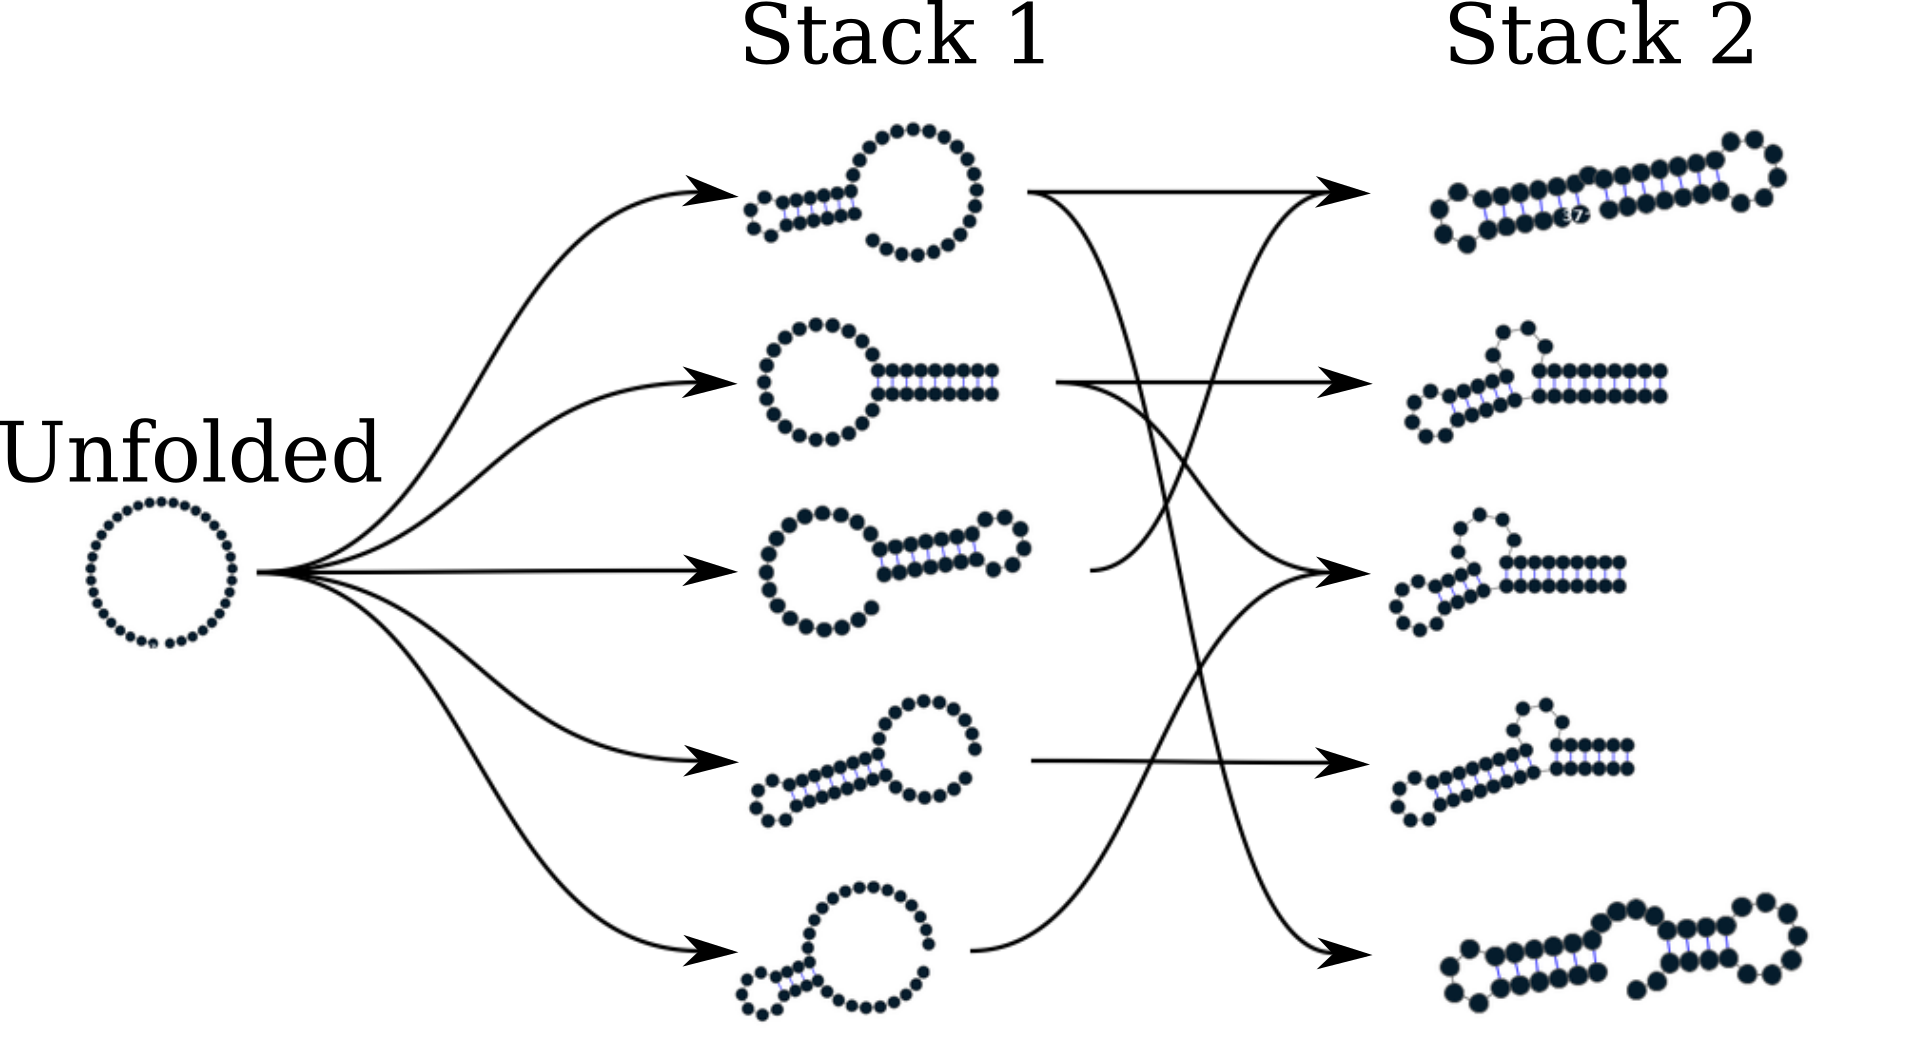
\includegraphics[width=1\linewidth]{../res/images/rafft/fast_paths_graph.png}
	\caption{\label{fast_path_graph}\textbf{Fast folding graph constructed using \texttt{RAFFT}.} In this example, the sequence is folded in two steps. The algorithm starts with the unfolded structure on the left. The \(N=5\) best stems are stored in stack 1. From stack 1, multiple stems formation are considered, but only the \(N=5\) best are stored in stack 2. Structures are ordered (from top to bottom) by energy in each stack. All secondary structure visualizations were obtained using \texttt{VARNA} \cite{darty09_varna}.}
\end{figure}


\begin{figure*}[t!]
	\centering
	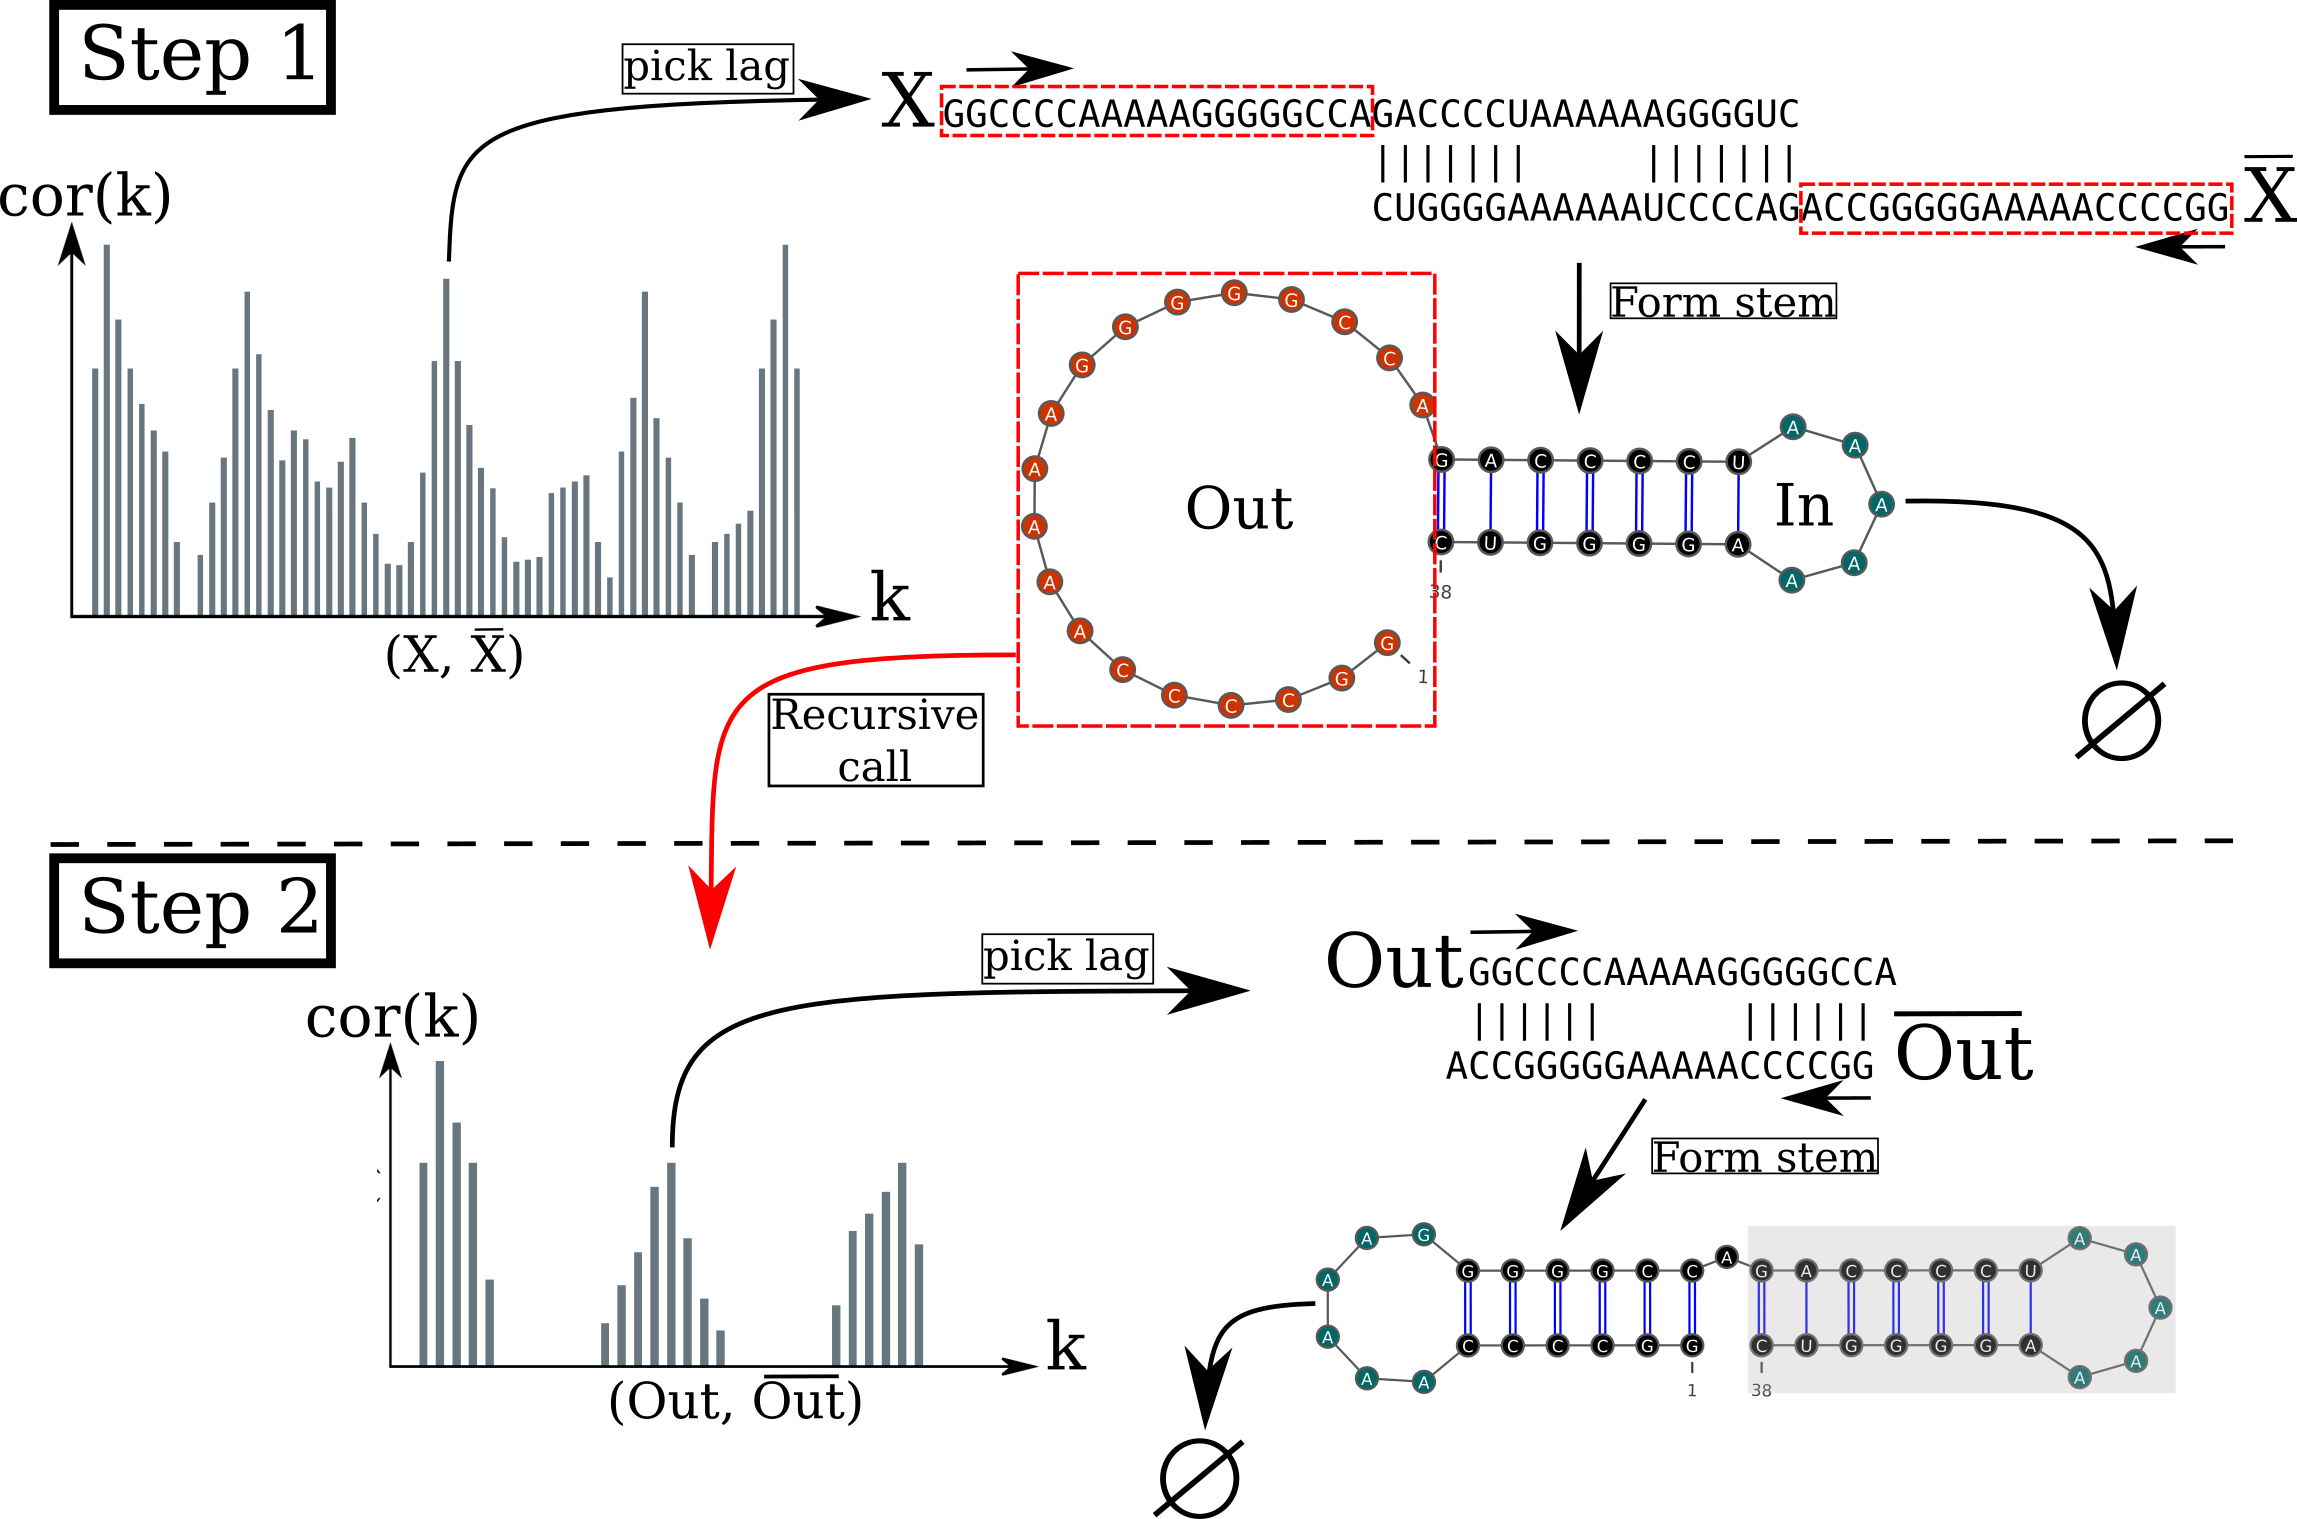
\includegraphics[width=.7\linewidth]{../res/images/rafft/algo_draw.png}
	\caption{\label{algo_desc}\textbf{Algorithm execution for one example sequence which requires two steps.} (Step 1) From the correlation $cor(k)$, we select one peak which corresponds to a position lag $k$. Then, we search for the largest stem and form it. Two fragments, ``In" (the interior part of the stem) and ``Out" (the exterior part of the stem), are left, but only the ``Out" may contain a new stem to add. (Step 2) The procedure is called recursively on the ``Out" sequence fragment only. The correlation $cor(k)$ between the ``Out'' fragment and its mirror is then computed and analyzing the $k$ positional lags allows to form a new stem. Finally, no more stem can be formed on the fragment left (colored in blue), so the procedure stops.}
\end{figure*}


To search for stems, we use the complementary relation between \(X\) and \(\bar{X}\) with the correlation function \(\text{cor}(k)\). This correlation is defined as the sum of individual \(X\) and \(\bar{X}\) row correlations:
\begin{equation}
\text{cor}(k)=\sum_{\alpha \in \{A,U,C,G\}}c_{X^{\alpha},\bar{X}^{\alpha}}(k),
\end{equation}
where a row correlation between \(X\) and \(\bar{X}\) is given by:
\begin{equation}
c_{X^\alpha,\bar{X}^\alpha}(k) = \sum\limits_{\substack{1\leq i \leq L\\1 \leq i + k \leq L}} \frac{X^\alpha(i) \bar{X}^\alpha(i+k)}{\text{min}(k, 2 L-k)}.
\end{equation}
For each \(\alpha \in \{A,U,C,G\}\), \(X^\alpha(i) \times \bar{X}^\alpha(i+k)\) is non zero if sites \(i\) and \(i+k\) can form a base pair, and will have the value of the chosen weight as described above. If all the weights are set to $1$, \(\text{cor}(k)\) gives the frequency of base pairs for a positional lag \(k\). Although the correlation naively requires \(O(L^2)\) operations, it can take advantage of the FFT which reduces its complexity to \(\mathcal{O}(L\;\text{log}(L))\).

Large \(\text{cor}(k)\) values between the two copies indicate positional lags \(k\) where the frequency of base pairs is likely to be high. However, this does not allow to determine the exact stem positions. Hence, we use a sliding window strategy to search for the largest stem within the positional lag (since the copies are symmetrical, we only need to slide over one-half of the positional lag). Once the largest stem is identified, we compute the free energy change associated with the formation of that stem. Next, we perform the same search for the \(n\) highest correlation values, which gives us \(n\) potential stems. Then, we define as the current structure the stem with the lowest free energy. Here, free energies were computed using Turner2004 energy parameters through ViennaRNA package API \cite{lorenz11_vienn_packag}.

We are now left with two independent parts, the interior and the exterior of the newly formed stem. If the exterior part is composed of two fragments, they are concatenated into one. Then, we apply recursively the same procedure on the two parts independently in a ``Breadth-First" fashion to form new consecutive base pairs. The procedure stops when no base pair formation can improve the energy. When multiple stems can be formed in these independent fragments, we combine all of them and pick the composition with the best overall stability. If too many compositions can be formed, we restrict this to the $10^4$ bests in terms of energy. Figure \ref{algo_desc} shows an example of execution to illustrate the procedure. 

The complexity of this algorithm depends on the number and size of the stems formed. The main operations performed for each stem formed are: (1) the evaluation of the correlation function \(\text{cor}(k)\), (2) the sliding-window search for stems, and (3) the energy evaluation. We based our approximate complexity on the correlation evaluation since it is the more computationally demanding step; the other operations only contribute a multiplicative constant at most. The best case is the trivial structure composed of one large stem where the algorithm stops after evaluating the correlation on the complete sequence. At the other extreme, the worst case is one where at most \(L/2\) stems of size $1$ (exactly one base pair peer stems) can be formed. The approximate complexity therefore depends on \(\sum_{i=0}^{L/2} (L-2i) \log(L-2i) \ = \mathcal{O}(L^2\log{L})\). Figure \ref{comp_plot} plots the execution time of a naive implementation of \texttt{RAFFT} and that of \texttt{RNAfold} for $20$ random sequences of various lengths, showing a substantial speed-up for larger sequences. 

The algorithm described so far tends to be stuck in the first local minima found along the folding trajectory. To alleviate this, we implemented a stacking procedure where the \(N\) best trajectories are stored in a stack and evolved in parallel. Figure \ref{fast_path_graph} illustrates this modified procedure. Like the initial version, the algorithm starts with the unfolded structure; then, the \(N=5\) best potential stems are stored in the first stack. From these \(N\) structures, the procedure tries to add stems in the unpaired regions left and saves the \(N\) best structures formed. Once no stem can be formed, the algorithm stops and output the structure with the best energy found among the structures stored in the last stack. This algorithm leads to the construction of a graph we call a \emph{fast-folding graph}. In this graph, two structures are connected if the transition from one to another corresponds to the formation of a stem or if the two structures are identical.

\begin{table*}[htbp]
	\caption{\label{average_perf}\textbf{Average performance displayed in terms of PPV and sensitivity.} The metrics were first averaged at fixed sequence length, limiting the over-representation of shorter sequences. The first two rows show the average performance for all the sequences for each method. The bottom two rows correspond to the performances for the sequences of length \(\leq\) $200$ nucleotides. For the ML and MFE only one prediction per sequence and for \texttt{RAFFT} $50$ predictions per sequence were used. Here \texttt{RAFFT} (respectively \texttt{RAFFT}*) refers to the case when the lowest free energy (resp. highest PPV) out of the $50$ predictions is selected.}
	\centering
	\begin{tabular}{lrrrr}
		\hline
		& \texttt{RAFFT} & \texttt{RAFFT}* & MFE  & ML\\
		\hline
		& \multicolumn{4}{c}{All sequences}\\
		\cmidrule{2-5}
		PPV         & 47.7  & 60.0   & 55.9 & 70.4\\
		Sensitivity & 52.8  & 62.8   & 63.3 & 77.1\\
		\hline
		& \multicolumn{4}{c}{Sequences with lengths \(\leq 200\)}\\
		\cmidrule{2-5}
		PPV         & 57.9  & 79.4   & 59.5 & 76.7\\
		Sensitivity & 63.2  & 81.2   & 65.5 & 82.9\\
		\hline
	\end{tabular}
\end{table*}

\subsection*{Kinetic ansatz}
The folding kinetic ansatz used here is derived from the fast-folding graph and allows us to model the slow processes in RNA folding. As described in Figure \ref{fast_path_graph}, transitions can occur from left to right (and right to left) but not vertically. The fast-folding graph follows the idea that parallel pathways quickly reach their endpoints; however, when the endpoints are non-native states, this ansatz allows slowly folding back into the native state \cite{pan97_foldin_rna_invol_paral_pathw}. 

As usually done, the kinetics is modelled as a continuous-time Markov chain \cite{lorenz20_effic_comput_base_probab_multi_rna_foldin}, where populations of structure evolve according to transition rates. In this context, an Arrhenius formulation is commonly used to derive transition rates \(r(x \rightarrow y) \propto \text{exp}(-\beta E^{\ddagger})\), where \(E^{\ddagger}\) is the activation energy separating \(x\) from \(y\), and \(\beta\) is the inverse thermal energy (mol/kcal). In contrast, our kinetic ansatz uses transition rates \(r(x\rightarrow y)\) based on the Metropolis scheme already used in \cite{klemm2008funnels}, and defined as
\begin{equation}
\label{Eq:metropolis}
r(x\rightarrow y) = k_0 \times \text{min}(1, \text{exp}(-\beta \Delta \Delta G(x\rightarrow y))),
\end{equation}
where \(\Delta \Delta G(x\rightarrow y)\) is the stability change between structure \(x\) and \(y\). Here \(k_0\) is a conversion constant that we set to $1$ for the sake of simplicity.  These transitions are only allowed if \(y\) is connected to \(x\) in the graph (i.e. \(y\) is in the neighborhood of \(x\), \(y \in \mathcal{X}\)). Here, we initialize the population \(p_x(0)\) with only unfolded structures; therefore, the trajectory represents a complete folding process. The frequency of a structure \(x\) evolves according to the master equation
\begin{equation}
\label{Eq:kenetics}
\frac{\text{d}p_x(t)}{\text{d}t} = \sum\limits_{y \in \mathcal{X}}
r(y \rightarrow x) p_{y}(t) - r(x \rightarrow y) p_{x}(t),
\end{equation}
where the sum runs over the neighborhood \(\mathcal{X}\) of \(x\).

The traditional kinetic approach starts by enumerating the whole space (or a carefully chosen subspace) of structures using \texttt{RNAsubopt}. Next, this ensemble is divided into local attraction basins separated from one another by energy barriers. This coarsening is usually done with the tool \texttt{barriers}. Then, following the Arrhenius formulation, one simulates a coarse grained kinetics between basins. In contrast, the Metropolis scheme used in our kinetic ansatz is based on the stability difference between structures, which may hide energy barriers. Due to this approximation, we referred to our approach as a `kinetic ansatz'.

\subsection*{Benchmark dataset}
To build the dataset for the folding task application, we started from the \texttt{ArchiveII} dataset derived from multiple sources \cite{andronescu08_rna_stran,brown98_ribon_p_datab,bellaousov10_probk,daub08_rna_wikip,damberger94_compar_datab_group_i_intron_struc,zwieb00_tmrdb,zwieb03_tmrdb,waring84_asses_model_intron_rna_secon,specht97_compil_rrna_rrna_gene_sequen,sprinzl98_compil_trna_sequen_sequen_trna_genes,sloma16_exact_calcul_loop_format_probab,schnare96_compr_compar_struc_charac_eukar,mathews99_expan_sequen_depen_therm_param,samuelsson99_signal_recog_partic_datab_srpdb,gutell93_compil_large_subun_like_ribos_rna_struc,gutell94_collec_small_subun_like_ribos_rna_struc,gardner09_rfam}. We first removed all the structures with pseudoknots, since the tools considered here do not handle these loops. Next, using the Turner2004 energy parameters, we evaluated the structures' energies and removed all the unstable structures: structures with energies $\Delta G_s > 0$. This dataset is composed of $2,698$ sequences with their corresponding known structures. $240$ sequences were found multiple times (from $2$ to $8$ times); $19$ of them were mapped to different structures. For the sequences that appeared with different structures, we picked the structure with the lowest energy. In the end we arrived at a dataset with $2,296$ sequences-structures.

\subsection*{Structure prediction protocols for benchmarks}
To evaluate the structure prediction accuracy of the proposed method, we compared it to two structure estimates: the MFE structure and the ML structure. To compute the MFE structure, we used \texttt{RNAfold 2.4.13} with the default parameters and the Turner2004 set of energy parameters. We computed the prediction using \texttt{Mxfold2 0.1.1} with the default parameters for the ML structure. Therefore, only one structure prediction per sequence for those two methods was used for the statistics.

Two parameters are critical for \texttt{RAFFT}, the number of positional lags in which stems are searched, and the number of structures stored in the stack. For our computational experiments, we searched for stems in the $n=100$ best positional lags and stored $N=50$ structures. The correlation function \(\text{cor}(k)\) which allows to choose the positional lags is computed using the weights \(w_{GC}=3\), \(w_{AU}=2\), and \(w_{GU}=1\).

To assess the performance of \texttt{RAFFT}, we analyzed the output in two different ways. First, we considered only the structure with the lowest energy found for each sequence. This procedure allows us to assess \texttt{RAFFT} performance in search of low energy structure only. Second, we computed the accuracy of all $N=50$ structures saved in the last stack for each sequence and displayed only the best structure in terms of accuracy. As mentioned above, the lowest energy structure found may not be the active structure. Therefore, this second assessment procedure allows us to show whether one of the pathways is biologically relevant.

We used two metrics to measure the prediction accuracy: the positive predictive value (PPV) and the sensitivity. The PPV measures the fraction of correct base pairs in the predicted structure, while the sensitivity measure the fraction of base pairs in the accepted structure that are predicted. These metrics are defined as follows:
\begin{equation}
PPV = \frac{TP}{TP + FP}, \;\;\; \text{Sensitivity} = \frac{TP}{TP+FN},
\end{equation}
where TP, FN, and FP stand respectively for the number of correctly predicted base pairs (true positives), the number of base pairs not detected (false negatives), and the number of wrongly predicted base pairs (false positives). To be consistent with previous studies, we computed these metrics using the \texttt{scorer} tool provided by Matthews \emph{et al.} \cite{mathews19_how_to_bench_rna_secon}, which also provides a more flexible estimate where shifts are allowed.

\subsection*{Structure space visualization}

We used a Principal Component Analysis (PCA) to visualize the loop diversity in the datasets considered here. To extract the weights associated with each structure loop from the dataset, we first converted the structures into weighted coarse-grained tree representation \cite{shapiro1990comparing}. In the tree representation, the nodes are generally labelled as E (exterior loop), I (interior loop), H (hairpin), B (bulge), S (stacks or stem-loop), M (multi-loop) and R (root node). We separately extracted the corresponding weights for each node, and the weights are summed up and then normalized. Excluding the root node, we obtained a table of $6$ features and \(n\) entries. This allows us to compute a \(6\times 6\) correlation matrix that we diagonalize using the \texttt{eigen} routine implemented in the \texttt{scipy} package. For visual convenience, the structure compositions were projected onto the first two Principal Components (PC). Figures \ref{perf_fig}C and \ref{perf_fig}D show the two principal components of the benchmark dataset, the predicted structure using \texttt{RAFFT}, \texttt{RNAfold} (MFE-structure) and \texttt{MxFold2} (ML-structure), where the arrows represent the direction of each feature in the PC space.


\begin{figure*}[t!]
	\centering
	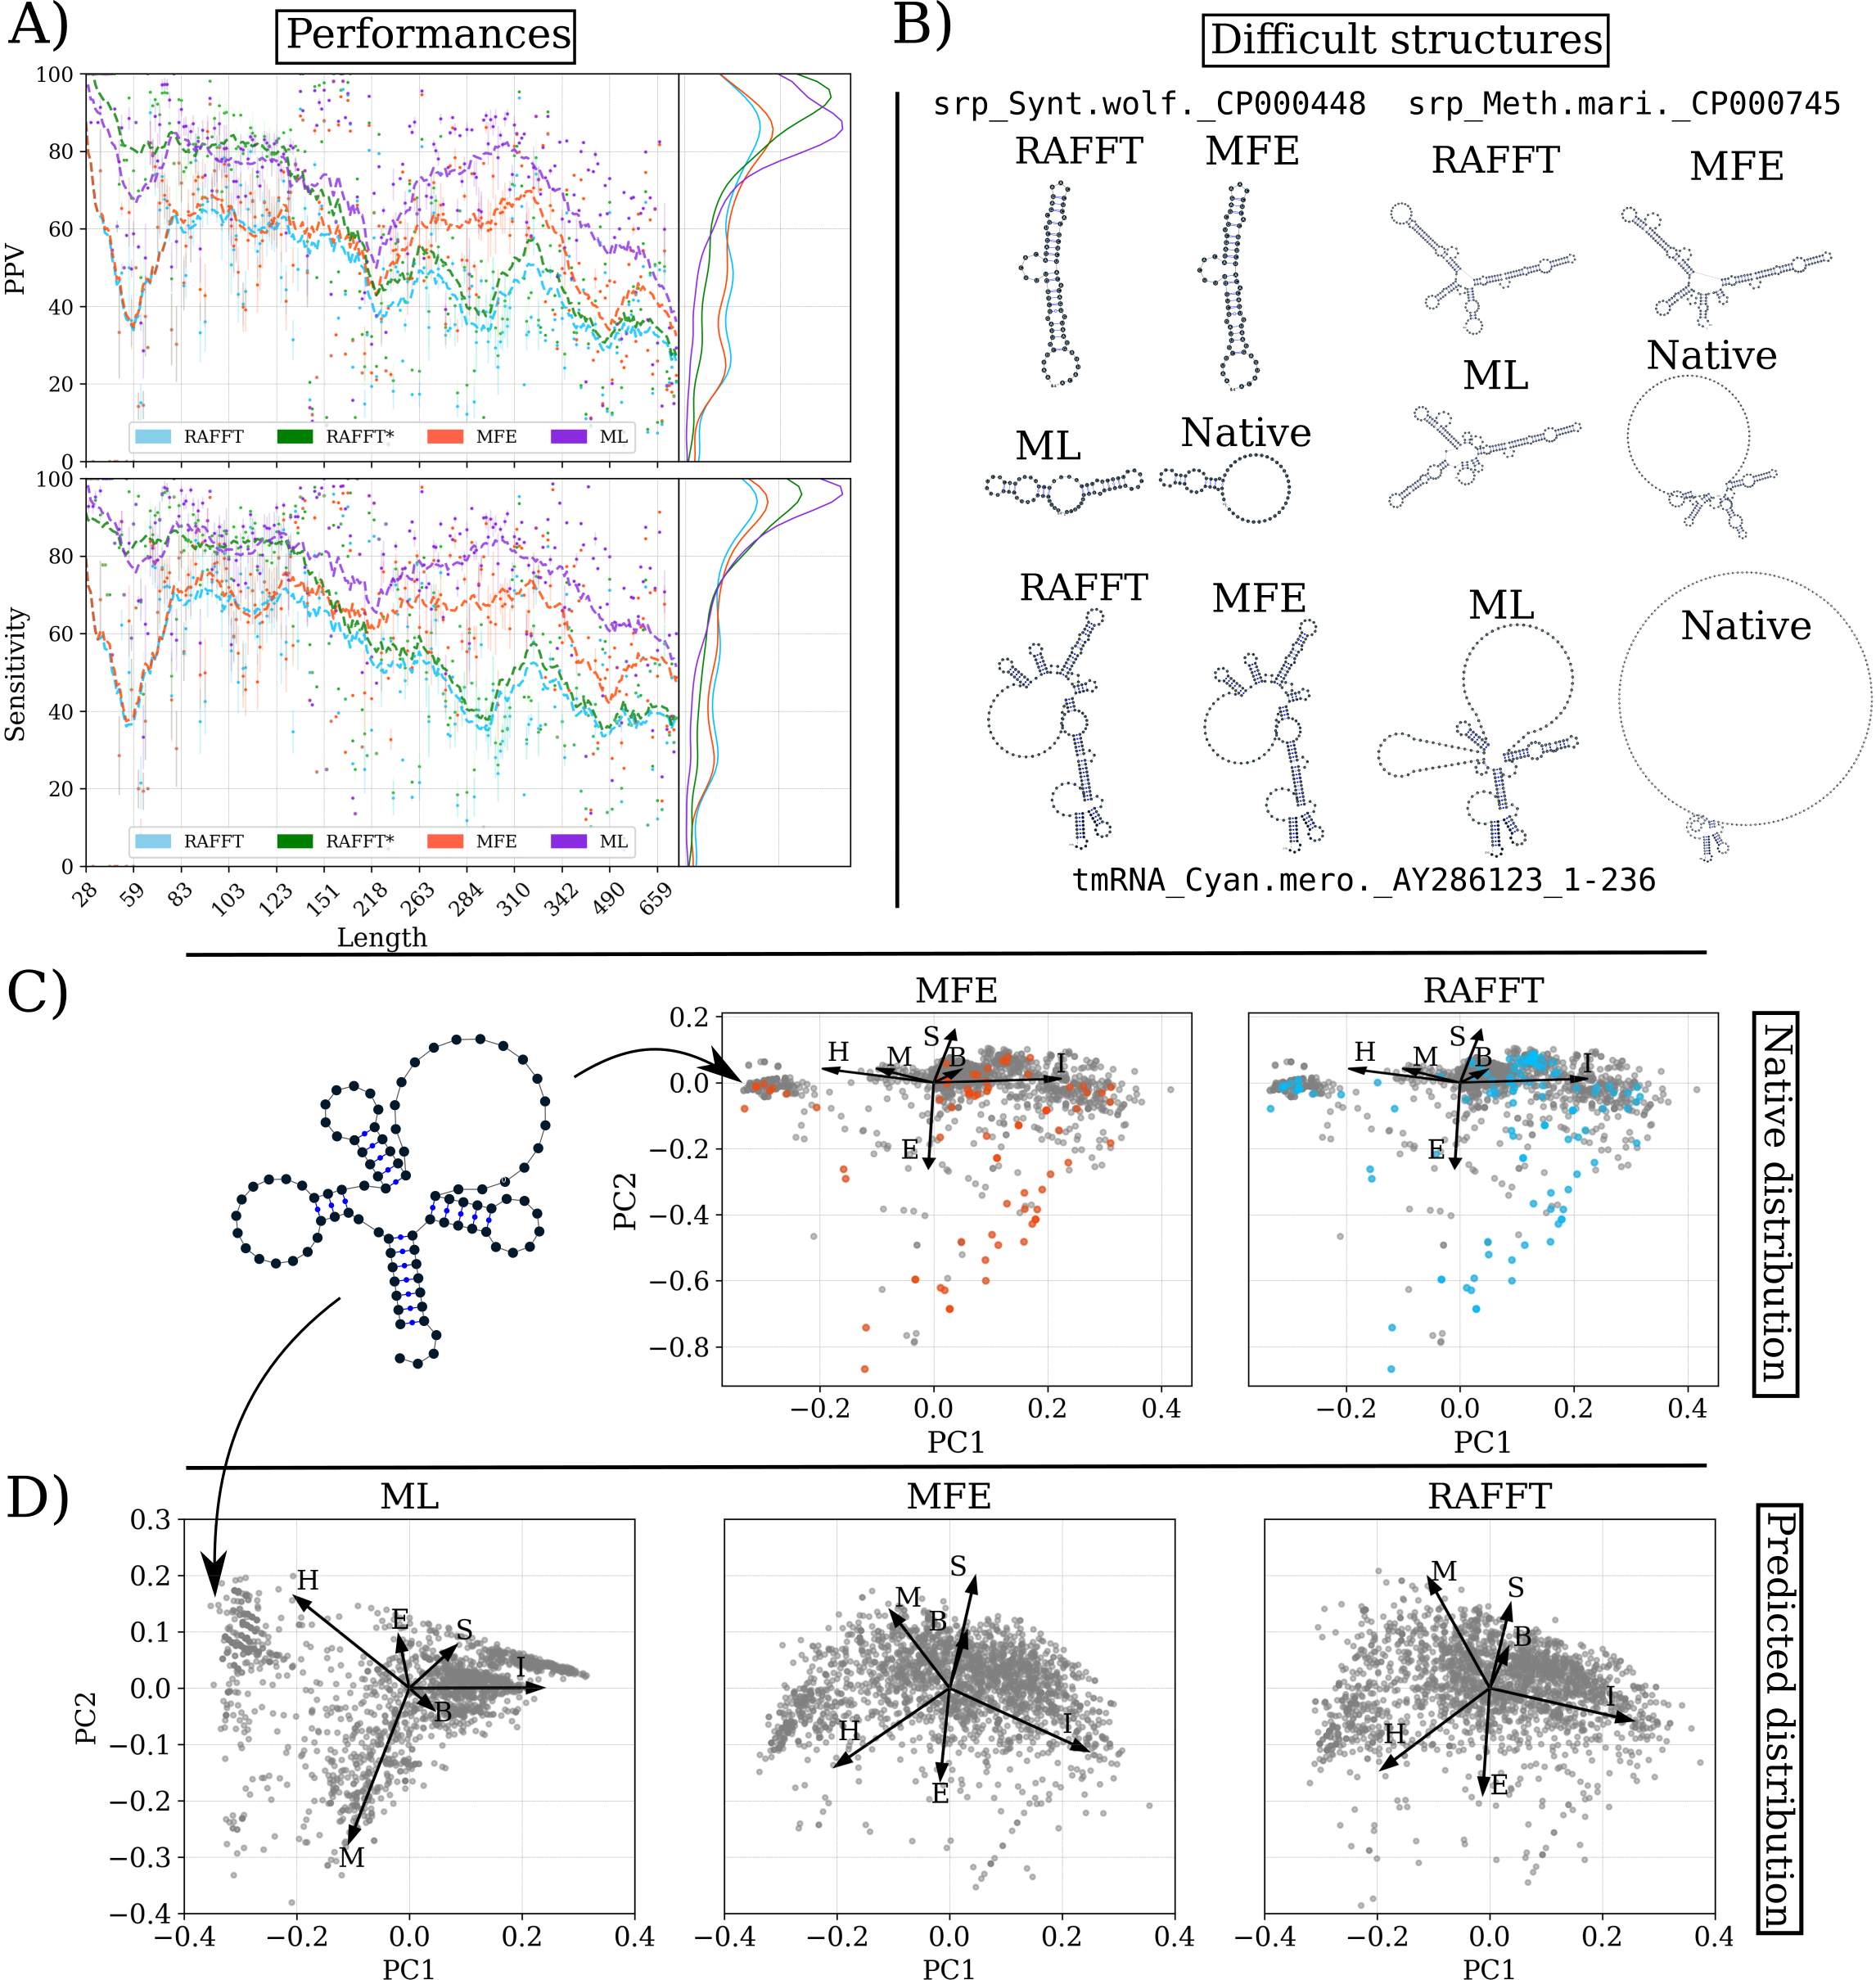
\includegraphics[width=.9\linewidth]{../res/images/rafft/perf_illed.png}
	\caption{\label{perf_fig} \textbf{\texttt{RAFFT}'s performance on folding task.} (A) PPV and sensitivity \emph{vs} sequence length. In the left panels, \texttt{RAFFT} (in blue) shows the scores when for the structure (out of $N=50$ predictions) with the lowest free energy, whereas \texttt{RAFFT}* (in green) shows the best PPV score in that ensemble. Each dot corresponds to the mean performance for a given sequence length, and vertical lines display their standard deviation. The right panels of both figures show the distribution of PPV and sensitivity sequence-wise. (B) List of structures that are challenging to predict using the thermodynamic model. The sequence names are from the dataset. The native structures have large regions with unpaired nucleotides. (C) PCA for structures in the dataset. An example of structures with a large hairpin (\textbf{H}) is shown on the left. The points marked in orange (resp. blue) are the MFE (resp. \texttt{RAFFT}) structures with PPV \(\leq\) \(10\%\). (D) PCA for the predicted structures. The MFE and \texttt{RAFFT} structure spaces look similar and more diverse than the ML structure space, closer to the native structure space.}
\end{figure*}

\section*{Results}
\subsection*{Application to the folding task}
We started by analyzing the prediction performances with respect to sequence lengths: we averaged the performances at fixed sequence length. Figure \ref{perf_fig}A shows the performance in predicted positive values (PPV) and sensitivity for the three methods. It shows that the ML method consistently outperformed \texttt{RAFFT} and MFE predictions. The $t$-test between the ML and the MFE predictions revealed not only a significant difference (p-value \(\approx\) $10$\textsuperscript{$-12$}) but also a substantial improvement of $14.5\%$ in PPV. \texttt{RAFFT} showed performances similar to the MFE predictions; however, \texttt{RAFFT} is significantly less accurate ($p$-value \(\approx\) $0.0002$), with a drastic loss of performance for sequences of length greater than $300$ nucleotides. In contrast, when only the most accurate predicted structure among the $50$ recorded structures per sequence was considered, we obtained $57.9\%$ of PPV and $63.2\%$ of sensitivity on average. The gain of performance was even more substantial for sequences of length below $200$ nucleotides. The PPV was $79.4\%$, and the sensitivity was $81.2\%$. In contrast, longer sequences did not display any gain. The average performances are shown in table \ref{average_perf}. We also investigated the relation to the number of bases between paired bases (base pair spanning), but we found no striking effect, as already pointed out in one previous study \cite{amman13_troub_long_range_base_pairs_rna_foldin}.

All methods performed poorly on two groups of sequences: one group of $80$ nucleotides long RNAs, and the second group of around $200$ nucleotides. Figure \ref{perf_fig}B shows three examples of such sequences. Both groups have large unpaired regions, which for the first group lead to structures with average free energies $9.8\ \textrm{kcal/mol}$ according to our dataset. The PCA analysis of the native structure space, shown in Figure \ref{perf_fig}C, reveals a propensity for interior loops and the presence of large unpaired regions like hairpins or external loops. Figure \ref{perf_fig}D shows the structure space produced by the ML predictions, which seems close to the native structure space. In contrast, the structure spaces produced by \texttt{RAFFT} and \texttt{RNAfold} (MFE) are similar and more diverse.

\begin{figure*}[t!]
	\centering
	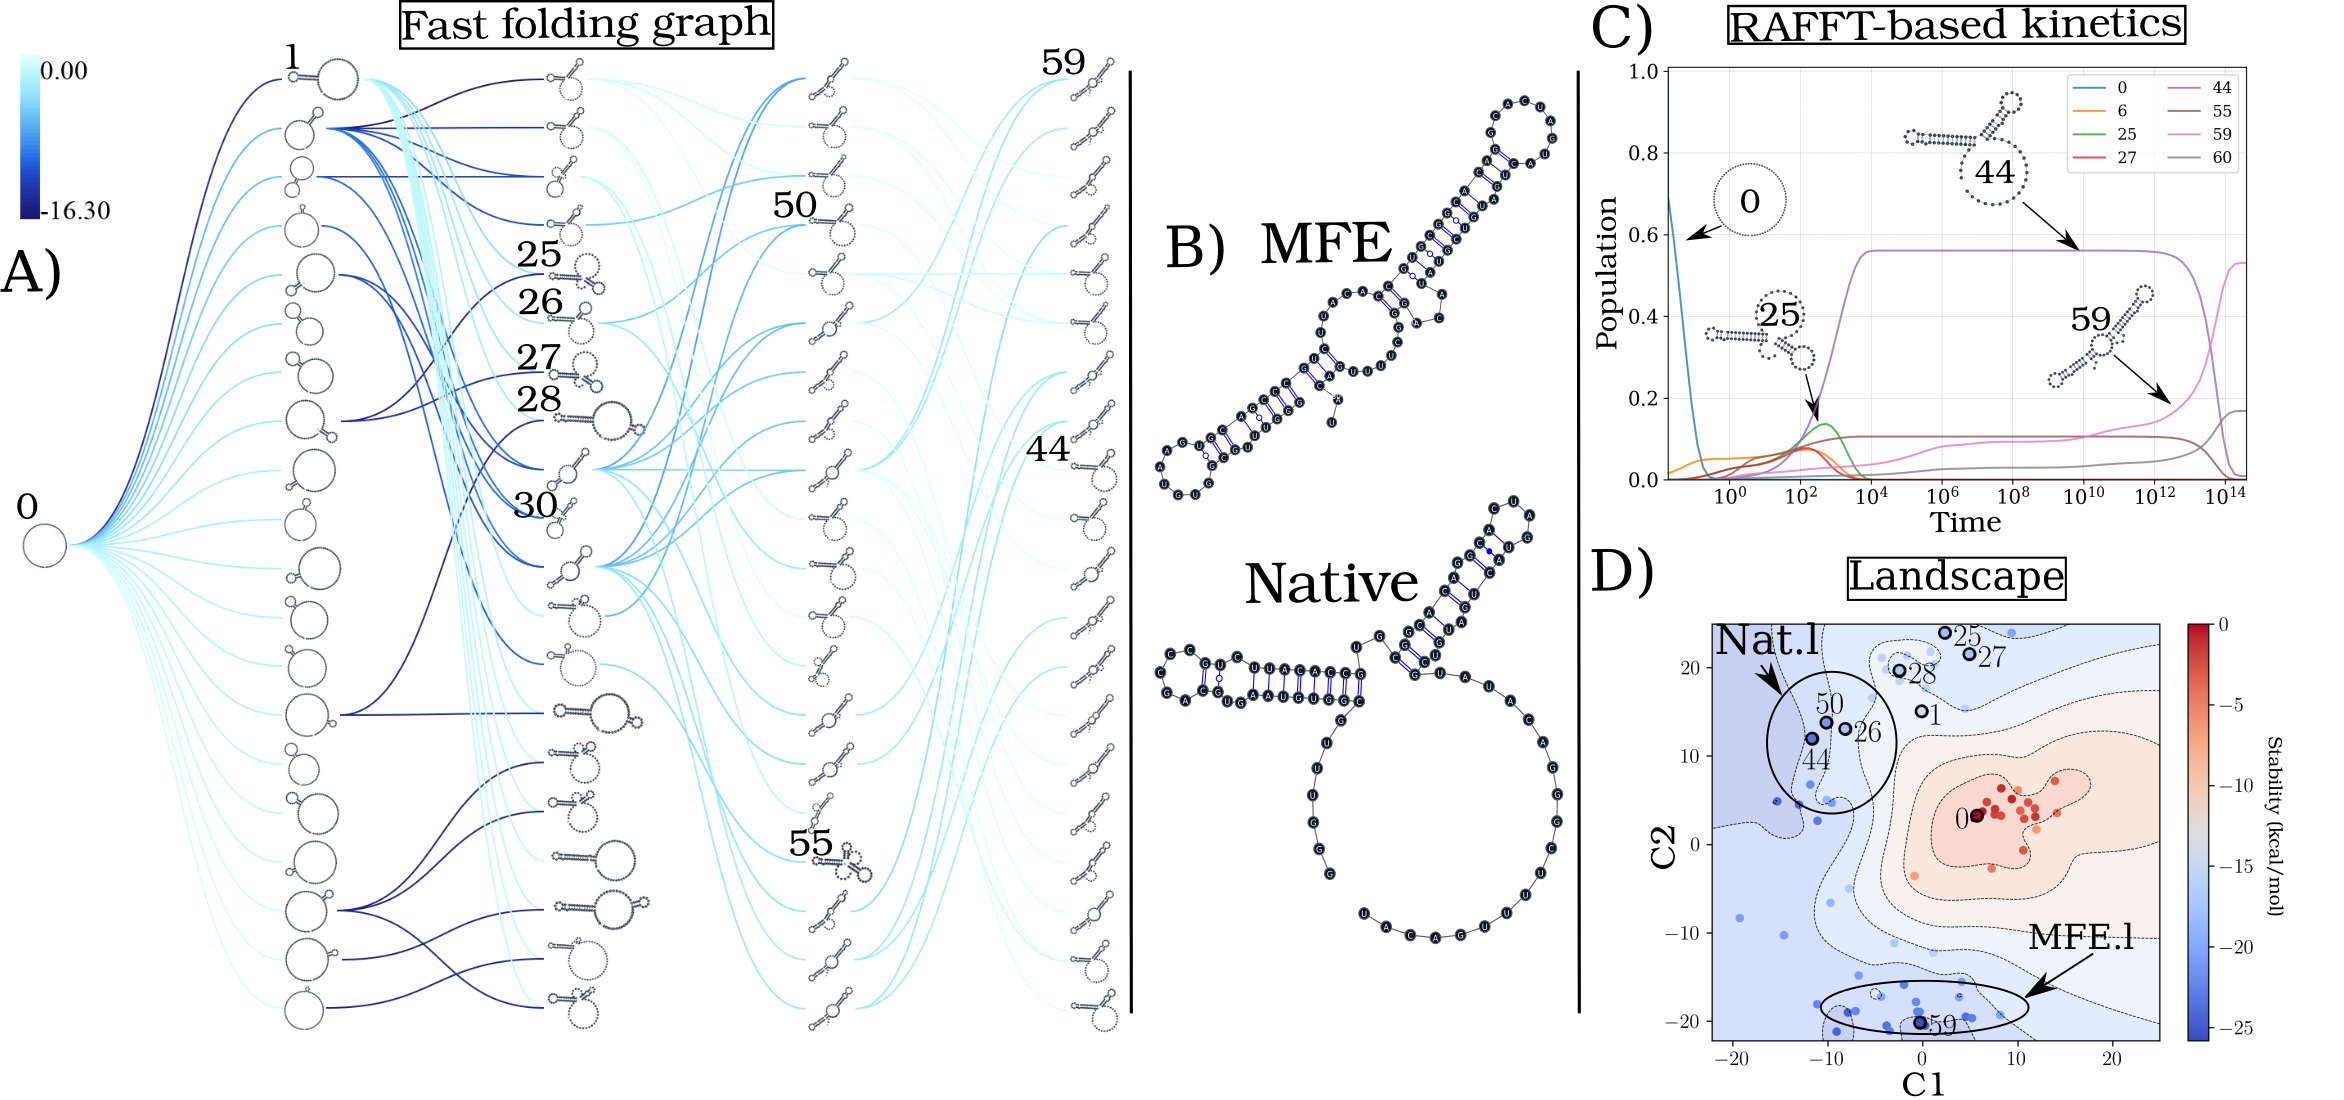
\includegraphics[width=0.9\linewidth]{../res/images/rafft/test_case.png}
	\caption{\label{test_case}\textbf{Application of the folding kinetic ansatz on CFSE.}  (A) Fast-folding graph in four steps and $N=20$ structures stored in a stack at each step. The edges are coloured according to \(\Delta \Delta G\). At each step, the structures are ordered by their free energy from top to bottom. The minimum free energy structure found is at the top left of the graph. A unique ID annotates visited structures in the kinetics. For example, ``$59$" is the ID of the MFE structure. (B) MFE (computed with \texttt{RNAfold}) and the native CFSE structure. (C)The change in structure frequencies over time. The simulation starts with the whole population in the open-chain or unfolded structure (ID 0). The native structure (\textbf{Nat.l}) is trapped for a long time before the MFE structure (\textbf{MFE.l}) takes over the population. (D) Folding landscape derived from the $68$ distinct structures predicted using \texttt{RAFFT}. The axes are the components optimized by the MDS algorithm, so the base pair distances are mostly preserved. Observed structures are also annotated using the unique ID. MFE-like structures (\textbf{MFE.l}) are at the bottom of the figure, while native-like (\textbf{Nat.l}) are at the top.}
\end{figure*}
\subsection*{Selected applications of the kinetic ansatz}
We started with the CFSE, a natural RNA sequence of $82$ nucleotides with a structure determined by sequence analysis and obtained from the RFAM database. This structure has a pseudoknot which is not taken into account here.

Figures \ref{test_case}A and \ref{test_case}B show respectively the fast-folding graph constructed using \texttt{RAFFT}, and the MFE and native structures for the CFSE. The fast-folding graph is computed in four steps. At each step, stems are constructed by searching for $n=100$ positional lags and, a set of $N=20$ structures (selected according to their free energies) are stored in a stack. The resulting fast-folding graph consists of $68$ distinct structures, each of which is labelled by a number. Among the structures in the graph, $6$ were found similar to the native structure ($16/19$ base pairs differences). The structure labelled ``$29$'' in the graph leading to the MFE structure ``$59$'' is the $9^{th}$ in the second stack. When storing less than $9$ structures in the stack at each step, we cannot obtain the MFE structure using \texttt{RAFFT}; this is a direct consequence of the greediness of the proposed method. To visualize the energy landscape drawn by \texttt{RAFFT}, we arranged the structures in the fast-folding graph onto a surface according to their base-pair distances; for this we used the multidimensional scaling algorithm implemented in the \texttt{scipy} package.  Figure \ref{test_case}D shows the landscape interpolated with all the structures found; this landscape illustrates the bi-stability of the CFSE, where the native and MFE structures are in distinct regions of the structure space.

From the fast-folding graph produced using \texttt{RAFFT}, the transition rates from one structure in the graph to another are computed using the formula given in Eq \ref{Eq:metropolis}. Starting from a population of unfolded structure and using the computed transition rates, the native of structures is calculated using Eq \ref{Eq:kenetics}. Figure \ref{test_case}C shows the frequency of each structure; as the frequency of the unfolded structure decreases to $0$, the frequency of other structures increases. Gradually, the structure labelled ``$44$", which represents the CFSE native structure, takes over the population and gets trapped for a long time, before the MFE structure (labelled "$59$") eventually becomes dominant. Even though the fast-folding graph does not allow computing energy landscape properties (saddle, basin, etc.), the kinetics built on it reveals a high barrier separating the two meta-stable structures (MFE and native). 

\begin{figure*}[t!]
	\centering
	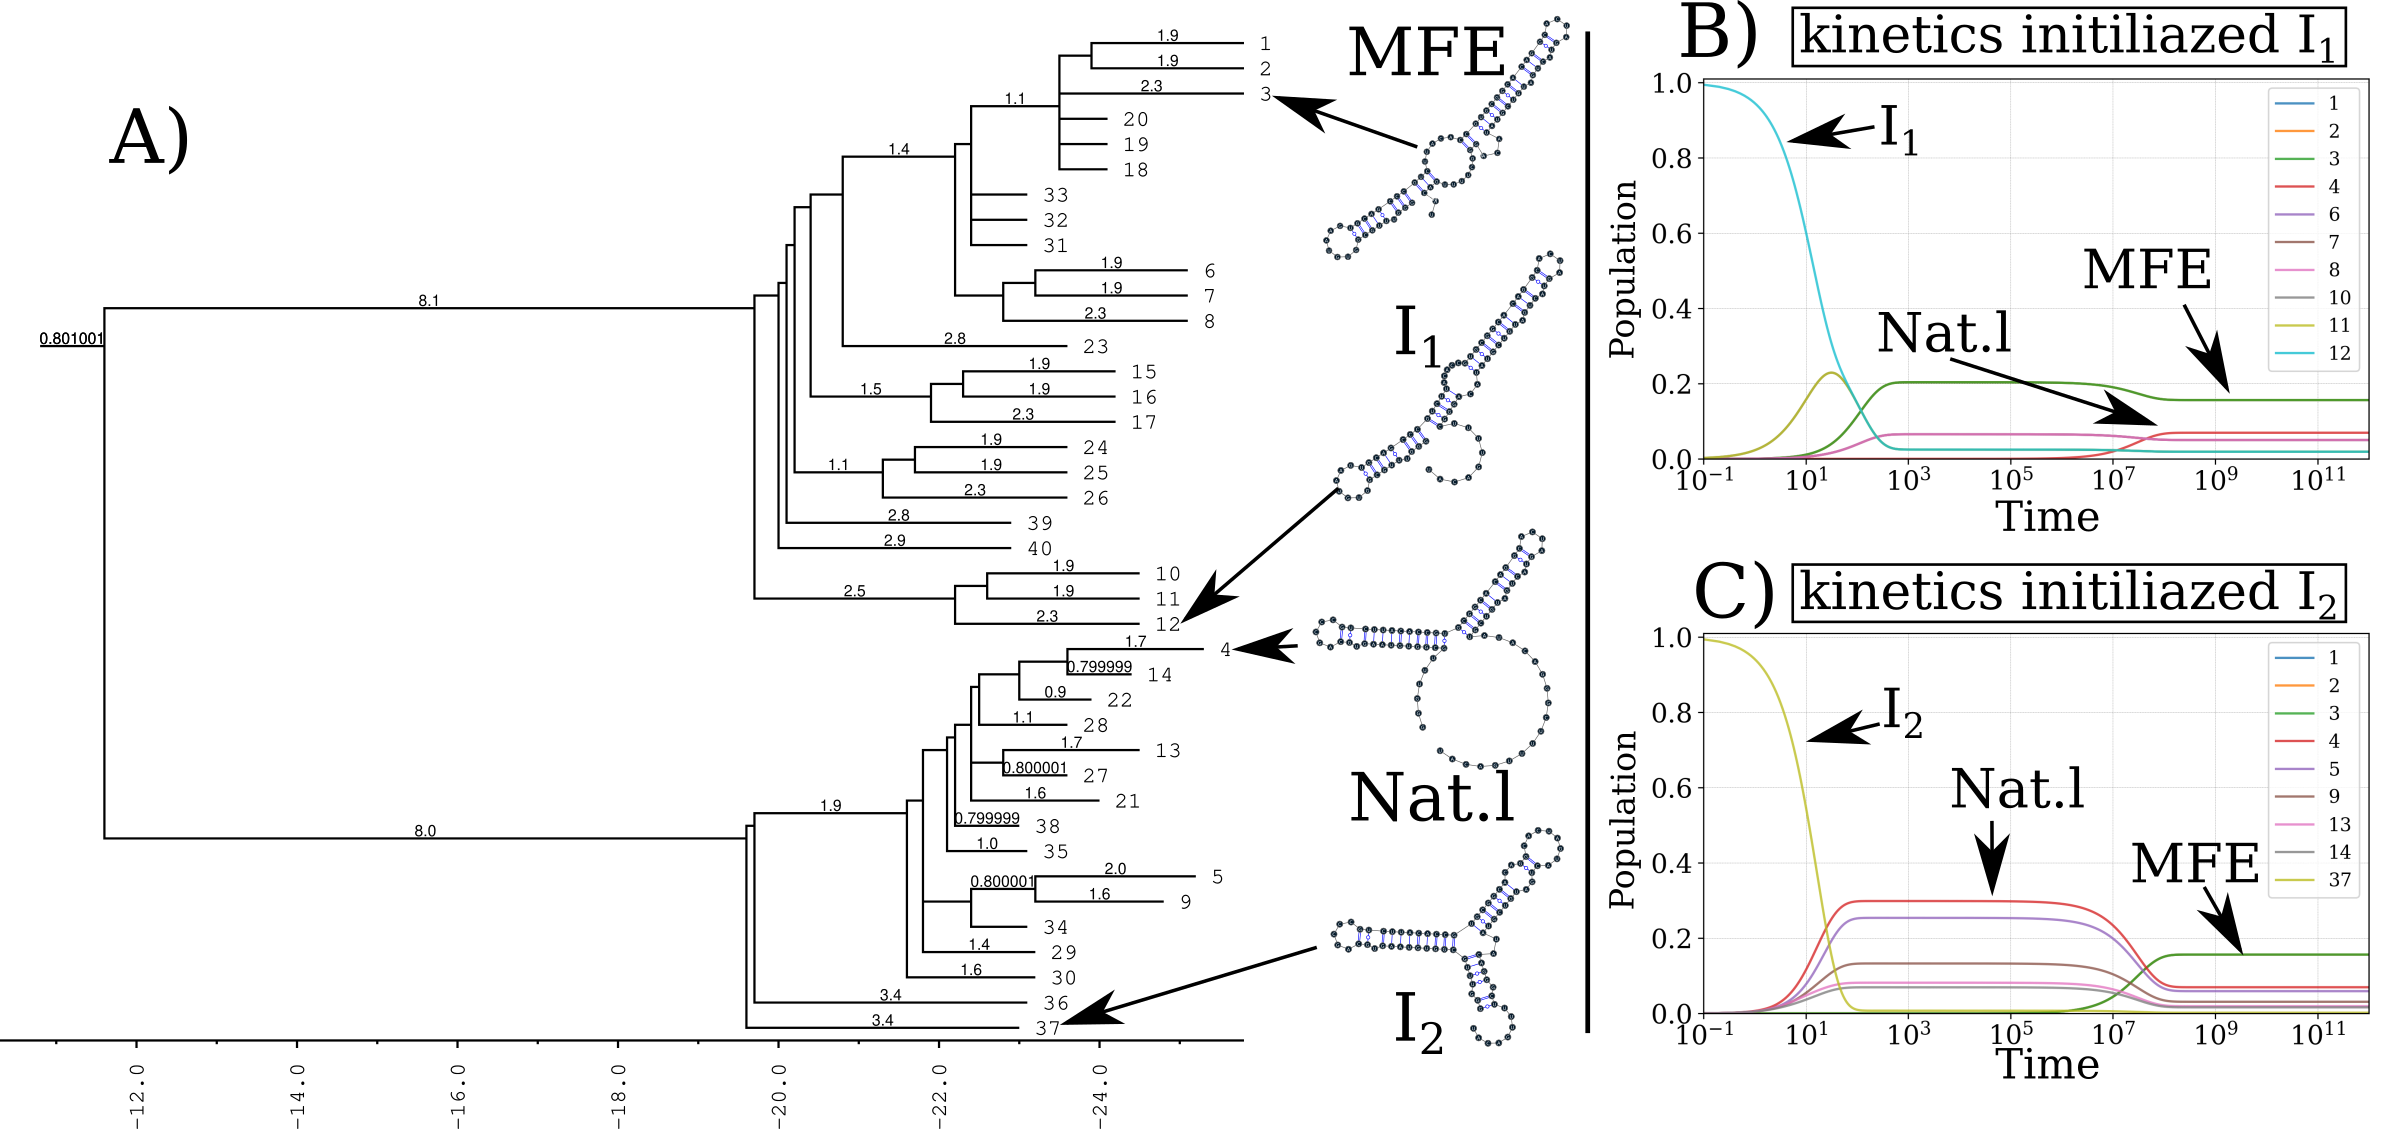
\includegraphics[width=0.9\linewidth]{../res/images/rafft/kinetic_treekin.png}
	\caption{\label{treekin}\textbf{Folding kinetics of CFSE using \texttt{Treekin}. }A) Barrier tree of the CFSE. From a set of $1.5\times10^6$ sub-optimal structures, $40$ local minima were found,  connected through saddle points. The tree shows two alternative structures separated by a high barrier with the global minimum (MFE structure) on the right side. (B) Folding kinetics with initial population $I_1$. Starting from an initial population of $I_1$, as the initial frequency  decreases, the others increase, and gradually the MFE structure is the only one populated.  (C) Folding kinetics with initial population $I_2$. When starting with a population of $I_2$, the native structure (labelled \textbf{Nat.1} ) is observable, and gets kinetically trapped for a long time due to the high energy barrier separating it from the MFE structure.}
\end{figure*}

Our kinetic simulation was then compared to \texttt{Treekin} \cite{flamm02_barrier_trees_degen_lands}. First, we generated \(1.5 \times 10^6\) sub-optimal structures up to $15 \ \textrm{kcal/mol}$ above the MFE structure using \texttt{RNAsubopt} \cite{lorenz11_vienn_packag}. Since the MFE is $\Delta G_s=-25.8 \ \textrm{kcal/mol}$, the unfolded structure could not be sampled. Second, the ensemble of structures is coarse-grained into $40$ competing basins using the tool \texttt{barriers} \cite{flamm02_barrier_trees_degen_lands}, with the connectivity between basins represented as a barrier tree (see Figure \ref{treekin}A). When using \texttt{Treekin}, the choice of the initial population is not straightforward. Therefore we resorted to two initial structures $I_1$ and $I_2$ (see Figure \ref{treekin}B and \ref{treekin}C, respectively). In Figure \ref{treekin}B, the trajectories show that only the kinetics initialized in the structure $I_2$ can capture the complete folding dynamics of CFSE, in which the two metastable structures are visible. Thus, in order to produce a folding kinetics in which the native and the MFE structures are visible, the kinetic simulation performed using \texttt{Treekin} required a particular initial condition and a barrier tree representation of the energy landscape built from a set of  $1.5 \times 10^6$ structures. By contrast, using the fast-folding graph produced by \texttt{RAFFT}, which consists only of $68$ distinct structures, our kinetic simulation produces complete folding dynamics starting from a population of unfolded structure.

As a second illustrative example, we applied both kinetic models to the classic bi-stable sequence \texttt{GGCCCCUUUGGGGGCCAGACCCCUAAAGGGGUC}. For \texttt{Treekin}, we first sampled the whole space of \(20 \times 10^3\) sub-optimal structures from the unfolded state to the MFE structure, and from that set, $40$ basins were also computed using \texttt{barriers}. The barrier tree in Figure \ref{class_examp} shows the bi-stable landscape, where the two deepest minima are denoted $S_A$ and $S_B$. As in the first application, we also chose two initializations with the structures denoted $I_1$ and $I_2$ in Figure \ref{class_examp}A and \ref{class_examp}B. Secondly, we simulate the kinetics starting from the two initial conditions (See Figure \ref{class_examp}B). When starting from $I_2$, the slow-folding dynamics is visible:  $S_B$ first gets kinetically trapped, and the MFE structure ($S_A$) only takes over later on. For our kinetic ansatz, we started by constructing the fast-folding graph using \texttt{RAFFT}, consisting of only $46$ distinct structures. The resulting kinetics, shown in Figure \ref{class_examp}B' was found qualitatively close to the barrier kinetics initialized with structure $I_2$. Once again, with few as $48$ structures, our proposed kinetic ansatz can produce complete folding dynamics starting from a population of unfolded structure.

\begin{figure*}[t!]
	\centering
	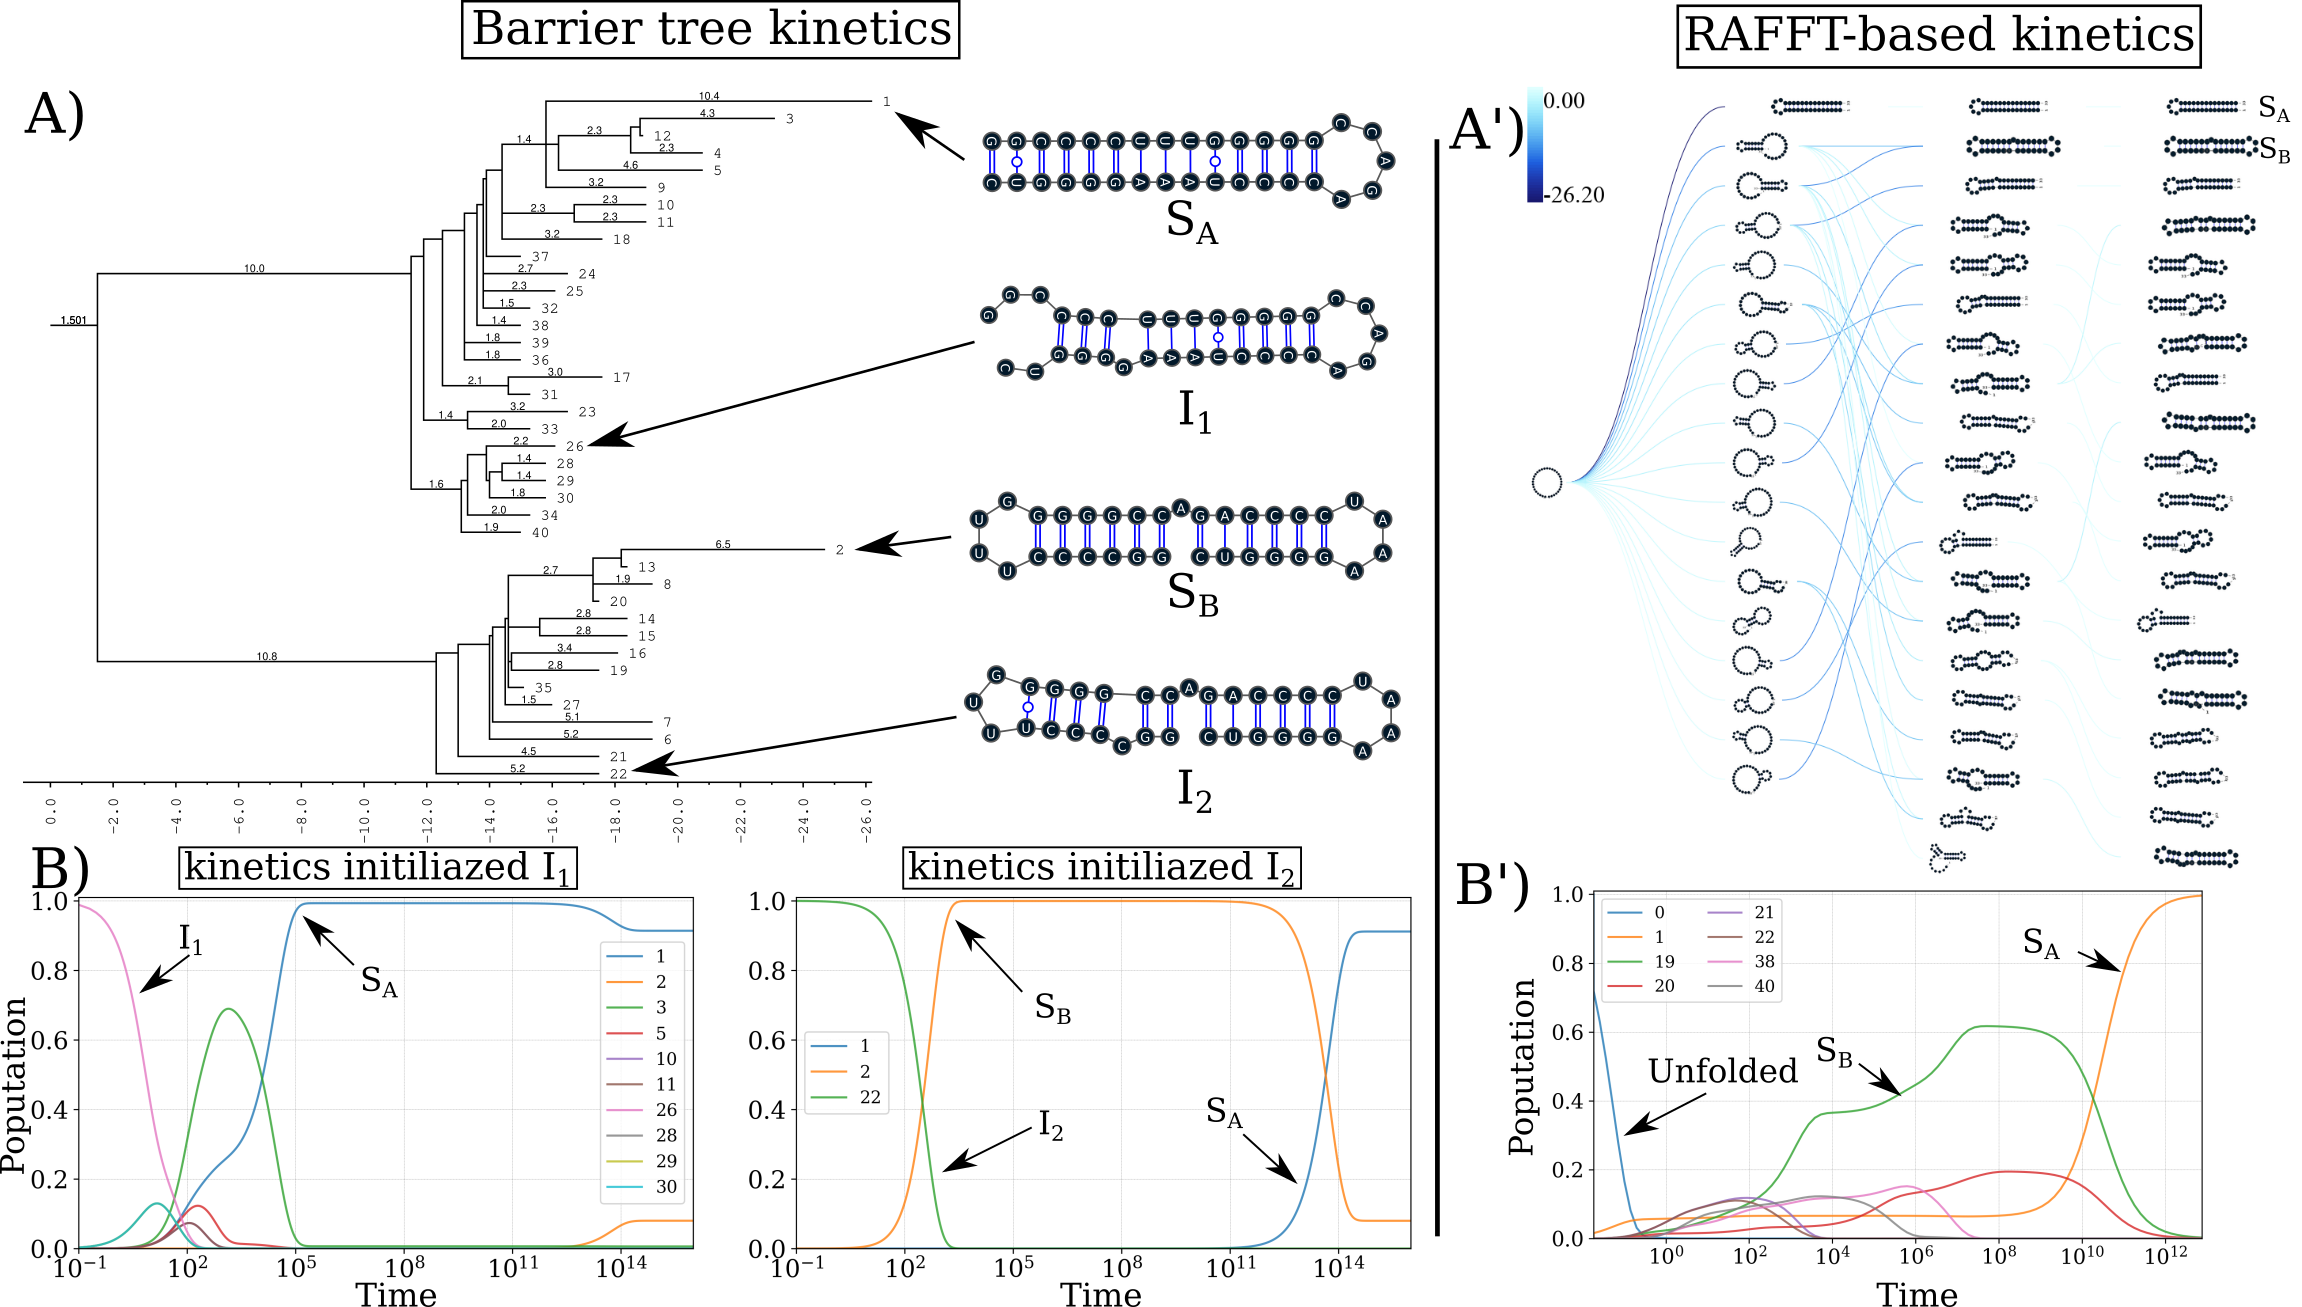
\includegraphics[width=0.9\linewidth]{../res/images/rafft/kine_bi_sta.png}
	\caption{\label{class_examp}\textbf{\texttt{RAFFT} \emph{vs} \texttt{Treekin}: folding kinetics of a bi-stable RNA sequence.} (A) Barrier tree for the bi-stable example sequence. The local minima and the corresponding barriers are computed from the complete enumeration of the structure space. The bi-stability is visible on the barrier tree through the two branches separated by a high barrier.  (B) Folding kinetics trajectories. The left plot shows the folding dynamics starting from a population with $I_1$, and the right size is the kinetics when the population is initialized in structure $I_2$. When starting from $I_1$, $S_A$ is quickly populated; starting from $I_2$, the bi-stability is more apparent.  (A') Fast-folding graph using \texttt{RAFFT}. A maximum of $N=20$ structures are stored in a stack at each step and overall $46$ distinct structures are visited. (B') Folding kinetics trajectory obtained from the fast-folding graph (indices are different from the barrier tree indices). The dynamics starts with a population with only unfolded structure, and slowly, $S_B$ is populated and gets trapped for a long time before the MFE structure $S_A$ becomes populated.}
\end{figure*}

\section*{Discussion}
We have proposed a method for RNA structure and dynamics predictions called \texttt{RAFFT}. Our method was inspired by the experimental observation of parallel fast-folding pathways. We designed an algorithm that produces parallel folding pathways, in which stems are formed sequentially, to mimic this observation. Then, to model the slow part of the folding process, we proposed a kinetic ansatz that exploits the parallel fast-folding pathways predicted.

First, we compared the algorithm performance for the folding task. Two structure estimates were compared with our method: the MFE structure computed using \texttt{RNAfold}, and the ML estimate using \texttt{MxFold2}. Other thermodynamic-based and ML-based tools were investigated but not shown here because their performances were found to be very similar to the one of \texttt{MxFold2} and \texttt{RNAfold} (See SI for the complete benchmark). When we considered the lowest energy structure, the comparison of \texttt{RAFFT} to existing tools confirmed the overall validity of our approach. In more detail, comparison with thermodynamic/ML models yielded the following results. First, the ML predictions performed consistently better than both \texttt{RAFFT} and the MFE approaches, where the PPV $=70.4\%$ and sensitivity $=77.1\%$ on average. Second, the ML methods produced loops, such as long hairpins or external loops. We argue that the density of those loops correlate with the ones in the benchmark dataset, which a PCA analysis revealed too. In contrast, the density of loops was lower in the structure spaces produced by \texttt{RAFFT} and MFE, implying some over-fitting in the ML model. Finally, known structures obtained through covariation analysis reflect structures \textit{in vivo} conditions. Therefore, the structures predicted by ML methods may not only result from their sequences alone but also from their molecular environment, e.g. chaperones. We expect the thermodynamic methods to provide a more robust framework for the study of sequence-to-structure relations.

With respect to MFE-based tools, we obtained a substantial gain of performance when analyzing \(N=50\) predicted structures per sequence and not only the lowest energy one. This gain was even more remarkable for sequences with fewer than $200$ nucleotides, reaching the accuracy of ML predictions. So how does \texttt{RAFFT} produce better structures, although these structures are less thermodynamically stable? The interplay of three effects may explain this finding. First, the MFE structure may not be relevant because active structures can be in kinetic traps. Second, \texttt{RAFFT} forms a set of pathways that cover the free energy landscape until they reach local minima, yielding multiple long-lived structures accessible from the unfolded state. Third, the energy function is not perfect, so that the MFE structures computed by minimizing it may not in fact be the most stable. 

We also showed that the fast-folding graph produced by \texttt{RAFFT} can be used to reproduce state-of-the-art kinetics, at least qualitatively. Our method demonstrated three main benefits. First, the kinetics can be drawn from as few as $68$ structures, whereas the barrier tree may require millions. Second, the kinetics ansatz describes the complete folding mechanism starting from the unfolded state. Third, for the length range tested here, the procedure did not require any additional coarse-graining into basins. (Longer RNAs might require such a coarse-graining step, in which structures connected in the fast-folding graph are merged together).

Based on our results, we believe that the proposed method is a robust heuristic for structure prediction and folding dynamics. The folding landscape depicted by \texttt{RAFFT} was designed to follow the kinetic partitioning mechanism, where multiple folding pathways span the folding landscape. This approach has shown good predictive potential. Furthermore, we derived a kinetic ansatz from the fast-folding graph to model the slow part of the folding dynamics. It was shown to approximate the usual kinetics framework qualitatively, albeit using many fewer structures. 

However, further improvements and extensions of the algorithm may be investigated. For starters, the choice of stems is limited to the largest in each positional lag, a greedy choice which may not be optimal. Furthermore, we have constructed parallel pathways leading to a diversity of accessible structures, but we have not given any thermodynamic-based criterion to identify which are more likely to resemble the native structure. We suggest using an ML-optimized score to this effect. Our method can also find applications in RNA design, where the design procedure could start with the identification of long-lived intermediates and use them as target structures. We also believe that mirror encoding can be helpful in phylogenetic analysis. Indeed, the correlation spectra \(\text{cor}(k)\) computed here contained global information of base-pairing that can be used as a similarity measure.



%\section*{Conclusions}

\section*{Data availability}
The implementation in \texttt{python3.0} of \texttt{RAFFT} and the benchmark data used in this manuscript are available at \url{https://github.com/strevol-mpi-mis/RAFFT}. We also provide the scripts used for the figures and kinetic analyses.
%\addtocontents{toc}{\protect\clearpage} % <--- just debug stuff, ignore
%************************************************
\chapter{\texttt{aRNAque}: An evolutionary algorithm for inverse folding inspired by Lévy flights.}\label{ch:arnaque}

Among the optimisation techniques presented in the previous chapter, the EA has demonstrated good statistical performance and provide an interesting framework for studying the evolutionary dynamics of biological systems. Since the genetic algorithm (or more generally evolutionary algorithm) was proposed by John Holland \cite{holland1992adaptation} in the early 1970s, it has emerged as a popular search heuristic and found application in many disciplines that deal with complex landscape optimization problems. Most of the evolutionary algorithms and stochastic search techniques are  guided by local (or one-point mutations) mutations. Although a local search can efficiently discover optima in a simple landscape, more complex landscapes pose challenges to the design of evolutionary algorithms that rely solely on local search. This is especially true on a landscape with high neutrality  where local search may be inefficient or risk getting stuck on a plateau (or local optimum). To avoid this pitfall, we propose here a new tool called \texttt{aRNAque} which implements a mutation scheme inspired by Lévy flights (called Lévy mutation) and supports pseudoknotted RNA target structures.

Lévy flights are random walks with a Lévy (or any heavy-tailed) step size distribution. The concept originates in the work of Mandelbrot on the fluctuation of commodities prices in the 1960s \cite{mandelbrot1972certain}, but has since found many more physical applications \cite{shlesinger1995levy}. The term "Lévy flight" was also coined by Mandelbrot, who used one specific distribution of step sizes (the Lévy distribution, named after the french mathematician Paul Lévy). Lévy flights also play a key role in the context of animal foraging, perhaps because they provide an optimal balance between exploration and exploitation \cite{viswanathan2008levy,kamaruzaman2013levy}. For a recent review of applications of Lévy flights in biology from the molecular to the ecological scale \cite{reynolds2018current}.

Similar to a Lévy flight, a Lévy mutation scheme allows simultaneous search at all scales over the landscape. New mutations most often produce nearby sequences (one-point mutations), but occasionally generate mutant sequences which are far away in genotype space (macro-mutations). In this work, the distribution of the number of point mutations at every step is taken to follow a Zipf distribution. 

In the coming sections, we provide a detailed description of \text{aRNAque} algorithm and the experimental result when compared to existing tools.

	
\section{Material and methods}

\subsection{Inverse folding evolutionary algorithm (EA)}
In general, an evolutionary search algorithm on any fitness landscape consists of three main parts, which in the context of RNA inverse folding are as follows: %(Figure \ref{Fig:model}):
\begin{itemize}
	\item Initialization: generating a random initial population of RNA sequences compatible with the given target secondary structure.
	\item Evaluation and selection: evaluating a population of RNA sequences consists of two steps: 1) fold each sequence into a secondary structure and assign it a weight based on its similarity to the target structure. 2) select a weighted random sample with replacement from the current population to generate a new population. A detailed description of the objective function used in \texttt{aRNAque} is provided in the next section. 
	\item Mutation (or move) operation: define a set of rules or steps used to produce new sequences from the selected or initial ones. This component is elaborated further in the next subsection.
	
\end{itemize}
%\begin{figure}[H]
%    \centering
%    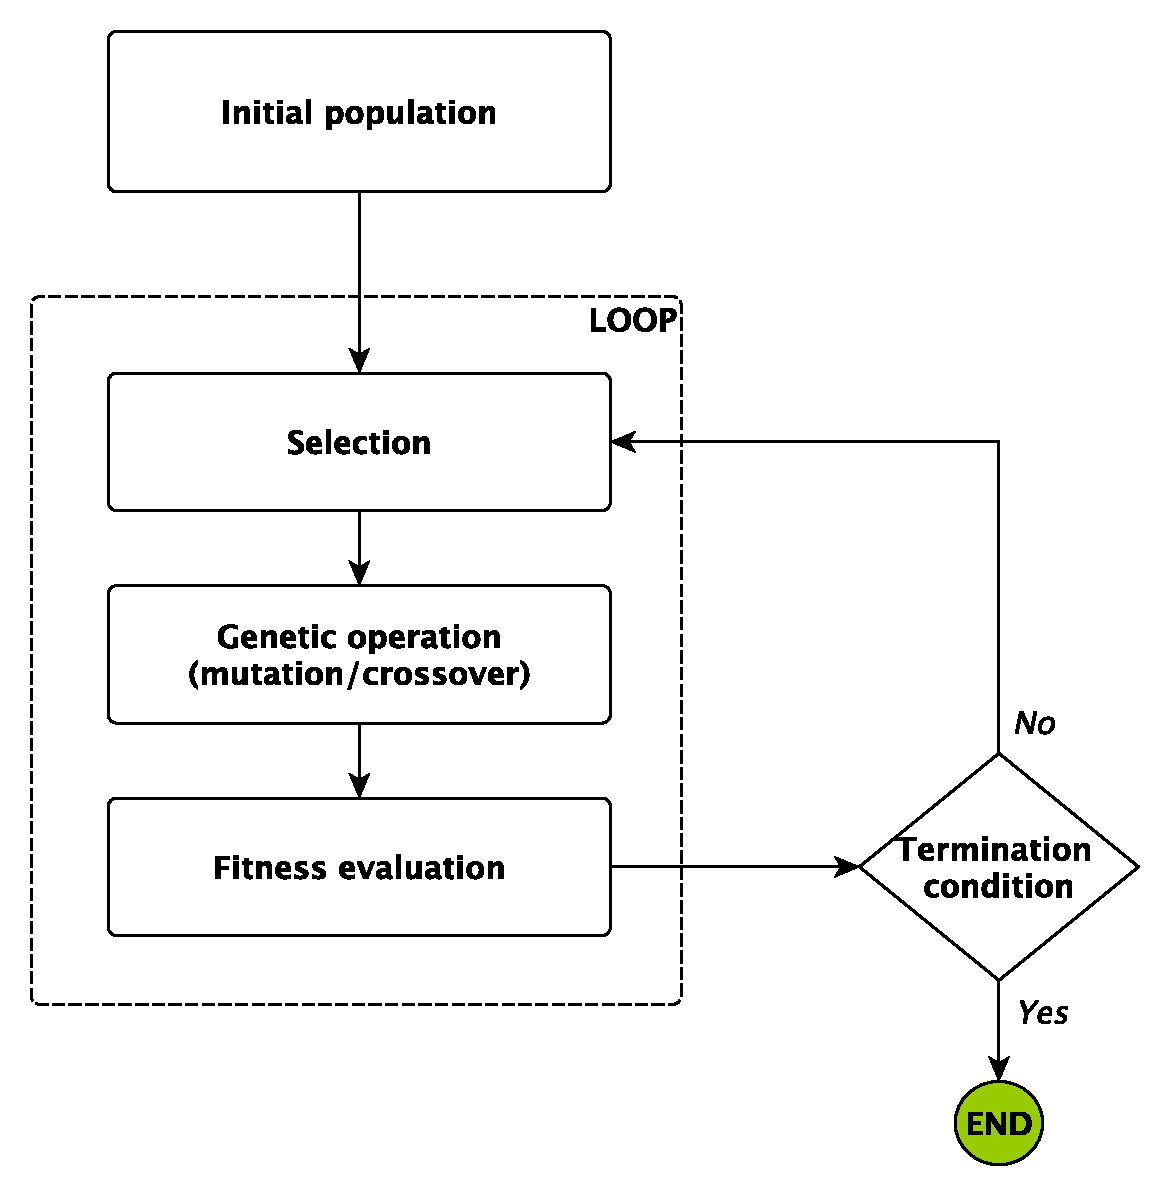
\includegraphics[width=0.5\textwidth]{figures/EA_draw.pdf}
%    \caption{Evolutionary algorithm flow diagram}
%    \label{Fig:model}
%\end{figure}


\subsection{\texttt{aRNAque}'s mutation operator}

For a given target RNA secondary structure $\sigma*$ of length $L$, the space of potential solutions to the inverse folding problem is $S=\{A,C,G,U\}^L$.
An evolutionary algorithm explores the space $S$ through its move (or mutation) operator. to explore exclusively the search space of compatible sequences (sequences with canonical base pairs at the corresponding open and closed bracket positions) with $\sigma^*$ , we introduce a mutation step that depends on the nucleotide and canonical base pair probability distribution.

Let~\(\mathcal{N}= \big \{ A, U, C, G \big \}\)~be the set of nucleotides weighted respectively by the probabilities:
\begin{equation*}
P_{\mathcal{N}} = \big \{ P_A, P_U, P_C, P_G \big\}
\end{equation*}
and~\(\mathcal{C} = \big \{ AU, UA, CG, GC, UG, GU\big \}\)~be the set of canonical base pairs weighted respectively by the probabilities:
\begin{equation*}
P_{\mathcal{C}} = \big \{P_{AU}, P_{UA},P_{CG},P_{GC},P_{UG},P_{UG} \big \} 
\end{equation*}
where
\begin{equation*}
\sum P_{\mathcal{N}} = 1, \sum P_{\mathcal{C}}  = 1 
\end{equation*}
and
\begin{equation*}
P_{AU} = P_{UA}, P_{UG} =P_{GU}, P_{CG} = P_{GC}
\end{equation*}
Therefore, our evolutionary algorithm relies on the flexibility of the mutation parameters $P_{\mathcal{N}}, P_{\mathcal{C}}$. These parameters allow the user to explicitly set the GC-content constraints , which allow the control of the nucleotide distribution during the design process.


\begin{figure*}[ht]
	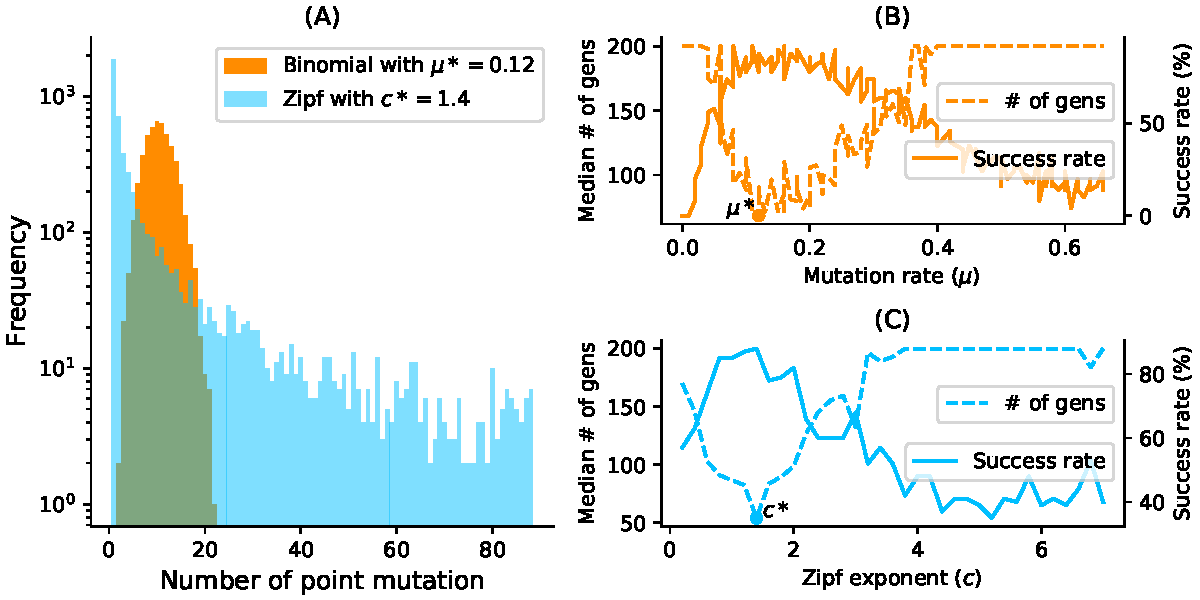
\includegraphics[width=1.0 \linewidth]{../res/images/arnaque/fig1.pdf}
	\caption{Binomial \emph{vs.} Zipf distributions. (A) Samplings Binomial and Zipf distributions for the best binomial mutation rate $\mu^*$ (respectively $c^*$ for the best Zipf exponent parameter). Both distributions have a mean of $8.7$ point mutations for a sequence of length $88$ nucleotides. (B) Tuning of binomial mutation rate parameter. For each $\mu \in [0,1]$ with a step size of $0.005$ and the pseudoknotted target \texttt{PKB00342} of length $88$, $50$ sequences were designed using \texttt{aRNAque}. (B) shows the median generations and the success percentage \emph{vs.} the mutation rate ($\mu$). The best mutation rate is $\mu^*=0.085$ (with a median number of generation $93.5$ and a success rate of $92\%$). (C) Tuning of Levy exponent. Similar to (B), for each $c \in [0,7]$ with a step size of $0.1$ and for the same pseudoknotted target structure, $100$ sequences were designed using \texttt{aRNAque}. It shows the median generations and the percentage of success \emph{vs.} the exponent parameter ($c$). The Zipf exponent distribution that produced the highest success rate and the minimum number of generations is $c^*=1.4$.}\label{Fig:histomut}. 
\end{figure*}
 We examined the binomial and Zipf distributions:

\begin{itemize}
	\item Binomial mutation: here $U$ has a binomial distribution: 
	$$
	P(U=n)= \binom{L}{n} \mu^n (1-\mu)^{L-n}
	$$
	for some $0 \leq \mu \leq 1$, such that $u=\mu \cdot L$. We can think of this mutation mode arising from each nucleotide of an RNA sequence independently undergoing a point mutation with probability $\mu$, i.e. $\mu$ is the per-nucleotide or point mutation rate. 
	
	\item Lévy mutation: $U$ has a Zipf distribution given by: 
	$$
	P(U=n)= \frac{1/n^c}{ \sum_{k=1}^{L}{1/k^c}}
	$$
	where $c>0$ is the value of the exponent characterizing the distribution.
\end{itemize}

Figure \ref{Fig:histomut} shows the distribution of the number of point mutations on a sequence of length $88$ nucleotides for both mutation schemes. Both distributions have the same mean, and the difference between the two distributions is more perceptible on their tails. 

In the rest of this work, a local mutation will refer to a binomial mutation with parameter $\mu \approx 1/L$.

We present the mutation algorithm in Algorithm \ref{Algo:Lévy}.

\begin{algorithm}
	\tcc{$P'=\{S'_1\dots S'_n\}$: the mutated population\; 
		$P= \{S_1\dots S_n\}$: a list of $n$ RNA sequences to mutate\;
		$P_{C}=\{w_{AU},w_{GU},w_{GC}\}$: a vector containing the weights associated with each canonical base pairs\;
		$P_{N}=\{w_{A},w_{U},w_{C}, w_{G}\}$: a vector containing the weights associated with each nucleotide\;
		$\mathcal{D}$: a given probability distribution (Lévy or Binomial) with parameter $p$ and $L$ where $L$ is the length of the target RNA structure}
	\KwInput{$P$, $\mathcal{D}(p, L)$, $P_{C}$,  $P_{N}$}
	\KwOutput{$P'$} 
	$ \{B_i\} \sim \mathcal{D}(p,L)$, where $i\in \{1,2,\dots,n\}$ \tcp*{Draw $n$ random numbers that follows a given distribution $\mathcal{D} (p,L)$ (Lévy or Binomial). $B_i$ is the number base pairs to mutate}
	$\{U_i\} \sim \mathcal{D}(p,L)$, where $i\in \{1,2,\dots,n\}$ \tcp*{Draw $n$ random numbers that follows the same distribution as $B_i$ (Lévy or Binomial). $U_i$ is the number non base pair positions to mutate}
	
	\For{ $i \in \{1, 2, \dots, n\}$ }{
		$S'\leftarrow P_i$ \tcp*{Assign the sequence $S_i \in P$ to $S'$ }
		\For{ $j \in \{1,2,...U_i\}$}{
			$r \in \{1,2,\dots, L\} \sim \mathcal{U}$ \tcp*{select uniformly a random position in the RNA sequence $S'$}
			$n_j \in \{A,U,C,G\} \sim P_N$ \tcp*{select a random nucleotide $n_j$ with respect to $P_N$} 
			$S'_r \leftarrow n_{j}$ \tcp*{replace the nucleotide at position $j$ in the RNA sequence $S'$ with $n_j$}
		}
		\For{ $j \in \{1,2,...B_i\}$}{
			$k_j \in \{AU,UA,CG,GC,GU,UG\} \sim P_C$ \tcp*{select a random base pair $k_{i}$ with respect to $P_C$}
			$b \in \{(b_1,b_2)_i\} \sim \mathcal{U}$ \tcp*{select uniformly a random pair of base pair positions}
			$S'_b \leftarrow k_{j}$ \tcp*{replace respectively the nucleotides at the base pair position $b_i \in b$ by $k \in k_j$}
			
		}
		$P' \gets P'\cup S'$ \tcp*{Add $S'$ to the list $P'$}
	}
	\caption{Mutation algorithm}\label{Algo:Lévy}
\end{algorithm}
%In addition to the two main features mentioned above, we also provide a web-server integrating an enriching interface to compare and analyse the designed sequences.

%%%%%%%%%%%%%%%%%%%%%%%%%%%%%%%%%%%%%%%%%%%%%%
%%                                          %%
%% Backmatter begins here                   %%
%%                                          %%
%%%%%%%%%%%%%%%%%%%%%%%%%%%%%%%%%%%%%%%%%%%%%%

\subsection{\texttt{aRNAque}'s objection functions}
Our EA reaches its performance through the minimization of three objective functions:

\begin{itemize}
	%\tightlist
	\item
	Hamming distance from the target structure:~since the main goal of the inverse folding problem is to find sequences that fold into a given target secondary structure~\(\sigma*\), the simple fitness measurement~\(f\) of an RNA sequence~\(\phi\)~can be defined as follows:
\end{itemize}

\begin{equation}
\label{fitness}
f(\phi, \sigma*) = \frac{1}{1 + d(s^{MFE}(\phi) , \sigma*)}
\end{equation}

where~\(d(\cdot,\cdot)\)~is the hamming distance on the structure space (structures are in dot and bracket representation).

\begin{itemize}
	%\tightlist
	\item
	Normalized Energy Distance (NED): the difference between
	the energy of a given sequence~\(\phi\)~evaluated to fold
	into a target structure~\(\sigma*\)~and the minimum free energy
	of the sequence in its structural ensemble~\(\Gamma\).~ The value is normalized over all the sequences in a given population $P$.  
\end{itemize}

\begin{equation}
\label{ned}
NED(\phi, \sigma*) = [1-\Delta E_{norm}(\phi, \sigma*)]^p \text{   } \forall p>1
\end{equation}
where,
\begin{equation}
\Delta E_{norm}(\phi, \sigma*) = \frac{\Delta E(\phi, \sigma*) }{\sum_{\phi \in P}{\Delta E(\phi, \sigma*)}}
\end{equation}
and,
\begin{equation}
\Delta E(\phi, \sigma*) = E(\phi, \sigma*) - \arg \min_{s \in \Gamma} E(\phi, s)
\end{equation}

\begin{itemize}
	%\tightlist
	\item
	Ensemble defect (ED) \cite{zadeh2011nucleic}: Here, we use the ED as a second objective function for refinement after having at least one sequence that folds into the target in the current population. It is defined in Equation \ref{ed}.
\end{itemize}


To minimize the $NED$ (Eq. (\ref{ned})) and the hamming distance (or maximize the fitness (Eq. (\ref{fitness})) of a population of RNA sequences, instead of combining both measurements to form a multi-objective function, we use them separately at a different level of our EA. We use the $NED$ as a selection weight for the sequences that will be mutated, and the hamming distance is used as a weight to elite ten best sequences that will always move to the next generation. Therefore the selection method we use is the \textit{fitness proportionate selection}, also known as roulette wheel selection \cite{lipowski2012roulette}. Once we have at least one sequence that folds into the given target in the current population (for the successful case), we walk through its neutral network by minimizing the ensemble defect function (Eq. (\ref{ed})). This ED minimization is simply performed by replacing the $NED$ objective function by the $ED$ function the EA (Step 4).

\subsection{\texttt{aRNAque}'s EA}

For a given population size $N$ and a target structure $\sigma*$ of length $l$, an initial population $P$ is generated randomly as follows: 

\begin{enumerate}
	\item Select randomly $l$ nucleotides in $N_{ucl.}$
	
	\item Identify the base pair position $(i,j)$ in the random sequence, select randomly a base pair in the set of canonical base pairs $C_{bp}$ and fix the first nucleotide of the selected canonical base pair at the position $i$ and the second at position $j$.
	
	\item  Repeat 2. for all base pair positions in the target structure
	
	\item Repeat 1. 2. and 3 $N-$times.
\end{enumerate}
Let \(T\) be the maximum number of generations and \(F_t\) the set of all sequences found at a given time ~\(t\). After the initial population of RNA sequences is generated, our algorithm is performed as follows:
\vspace{0.05cm}

\(\texttt{While}\) \((t<T)\)~or~\( |F_t| <n_f\)
\(\texttt{do}\) :

\begin{itemize}
	%\tightlist
	\item Evaluate the fitness (Eq. (\ref{fitness})) of every sequence \(s \in P\)
	\item
	Add to \(F_t\)~all the sequences with fitness equal to $1$
	\item
	Choose~\(10\)~best sequences of~\(P\)~based
	on their fitness (Eq. (\ref{fitness})) values and add them to \(P'\)~.
	\item
	Sample~\(N\) sequences with respect to their \textit{NED} (Eq. (\ref{ned})) values and store them in~\(S\).
	\item
	\(\texttt{For}\) each RNA sequence ~\(s \in S\):~
\end{itemize}

\begin{quote}
	\begin{enumerate}
		%\tightlist
		\item
		\(s'\) = \(\texttt{copy(s)}\)~
		\item
		Select a random nucleotide~\(r_n
		\)
		in~\(N_{ucl.}\)~respect to the
		probabilities~\(P_{nucl.}\)~
		\item
		\(s'[i] = r_n\), where~\(i\)~is a random integer
		chosen uniformly from \(0\)~to \(l-1\)~
		\item
		Select a random base paire~\(b_p
		\) in~\(C_{bp}\)~
		respect to the probalities~\(P_{can.}
		\)
		\item
		\(s'[i] \leftarrow b_p[0]\)~and \(s'[j] \leftarrow b_p[1]\), where \((i,j)\)
		is a random tuple of integers chosen uniformly from the set of base
		pair positions.~
		\item
		Add~\(s'\) in \(P'\)~
	\end{enumerate}
\end{quote}

\begin{itemize}
	%\tightlist
	\item
	\(P \leftarrow P'\)
	\item
	\(t \leftarrow t + 1\)
\end{itemize}

\subsection{Parameter analysis and benchmark data}
Here we analyse mutation parameters and compare local and Lévy mutation modes. 

\subsubsection{Benchmark data used}
The \texttt{PseudoBase++} is a set of $266$ pseudoknotted RNA structures used to benchmark \texttt{Modena}. It was initially $342$ RNA secondary structures, but because of the redundancy and the non-canonical base pairs  $76$ structures were excluded. To group the dataset with respect to the pseudoknot motifs (Figure \ref{Fig:pk_type}), we used the test data from \texttt{antaRNA}'s paper. The test data contains $249$ grouped into four categories: $209$ hairpin pseudoknots (H), $29$ bulge pseudoknots (B), $8$ complex hairpin pseudoknots (cH) and $3$ kissing hairpin pseudoknots (K). Out of the $266$ structures, only $185$ (with $150$ H-type, $3$ K-type, $25$ B-type and $7$ cH-type) structures were included in the test data. So for that reason, we have used only $185$ target structures for the pseudoknot motif performance comparison and the $266$ structures for the different target lengths performance comparison.

The \(\texttt{Eterna100}\) dataset \cite{Eterna} is available in two versions and both contain a set of \(100\) target structures extracted from the \texttt{EteRNA} puzzle game and classified by their degree of difficulty. The \texttt{Eterna100-V1} was initially designed using \texttt{ViennaRNA} 1.8.5, which relies on Turner1999 energy parameters \cite{Turn1999}. Out of the $100$ target secondary structures, $19$ turned out to be unsolvable using the version of \texttt{ViennaRNA} $2.4.14$ (which relays on the Turner2004 \cite{mathews2004incorporating}). Subsequently, an \texttt{Eterna100-V2} \cite{Eterna} was released in which the $19$ targets were slightly modified to be solvable using \texttt{ViennaRNA} $2.4.14$ and any version that supports the Turner2004 energy parameters. The main difference between the two dataset relay on the energy parameters used to generate the data.

The \texttt{non-EteRNA} dataset: a set of \(63\) experimentally synthesized targets that Garcia-Martin et al. \cite{garcia2013rnaifold} recently used to benchmark a set of ten inverse folding algorithms, which from our knowledge, is the most recent and comprehensive benchmark of current state-of-the-art methods. The dataset is collected from \(3\) sources: the first dataset called \(\textbf{dataset A}\) which contains \(29\) targets collected from RFAM and also used in \cite{esmaili2015erd,taneda2011modena} and the second called \(\textbf{dataset B}\) is a collection of \(24\) targets used in \cite{esmaili2015erd} and added to that the \(10\) structures used in \cite{shi2018sentrna}.

\subsection{Benchmark protocol}
\subsubsection*{Folding tools}
Two tools for pseudoknotted RNA folding are considered in this work: \texttt{HotKnots} and \texttt{IPknot}. For pseudoknot-free RNA folding, we used \texttt{RNAfold}.
 For the mutation parameter and GC-content analysis presented in our work, we used \texttt{IPknot}, and both \texttt{HotKnots} and \texttt{IPknot} for \texttt{PseudobBse++} benchmarks. To be able to use \texttt{HotKnots} in \texttt{aRNAque} without copying \texttt{aRNAque} in the bin directory of \texttt{Hotknots}, we have performed some modifications on \texttt{Hotknots} source code. Details on the modifications are provided in the supplementary material SI 6. Furthermore, we considered \texttt{pkiss}, a well known tool for K-type pseudoknot prediction, but since the \texttt{PseudoBase++} dataset contains just $4$ K-type pseudoknotted structures and \texttt{pKiss} has higher time complexity ($O(n^6)$), we did not find it efficient for the benchmark we performed.
\subsubsection*{Mutation parameters tuning}
One of the main challenges for an evolutionary algorithm is to find optimum parameters such as mutation rate, population size and selection function.
We used $80$ pseudoknotted targets with lengths from $25$ to $181$ nucleotides for the mutation parameter analysis. We set the maximum number of generations $T$ to $200$ and the population size $n$ to $100$. The stopping criteria are two: 1) the number of generations ($t$) is equal to the max number of generations ($T$) or 2)the minimum hamming (or base pair) distance of the best RNA sequence solution to the target is $0$. The best mutation parameters ($c^*$ for Levy and $\mu^*$ for Binomial) are those that have the lowest median number of generations. The best mutation parameters obtained for both binomial and Lévy mutation modes are used to benchmark and compare the results on the entire datasets of RNA structures.
\subsubsection*{Benchmark on the \texttt{PseudoBase++} dataset}
Four benchmarks are performed on the pseudoknotted dataset: 1) mutation parameter analysis, 2) the GC-content and diversity analysis, 3) Local search versus Lévy search, 4) \texttt{aRNAque} (Lévy search) versus \texttt{antaRNA}. For the \texttt{aRNAque} (Binomial and Lévy) case, the four benchmarks share the same number maximum number of generations ($T=200$), population size ($n=100$), stopping criteria ($t=T$ or min fitness equals $0$).
For the \texttt{antaRNA} benchmark, the maximum number of iterations was set to $1200$, and a slight modification was made to allow the support of the folding tool $\texttt{HotKnots}$ (See SI 6).  
For booth tools and each benchmark,  $20$ runs were launched independently in parallel on a computer with the same resources, resulting in $20$ designed sequences per pseudoknotted target structure. To measure the performance of each tool, each designed sequence $s$ is folded into a secondary structure $\sigma$ and the similarities between $\sigma$ and $\sigma^*$ are computed using the base pair distance. 
For the GC-content benchmark, four GC-content values are considered, $\{0.25, 0.5, 0.75,1\}$ and the setting of each tool remains the same.
\subsubsection*{Benchmark on the \texttt{Eterna100} dataset}
We performed two benchmarks are one the \texttt{Eterna100} dataset: 1) a benchmark on the \texttt{Eterna100-V1} dataset using the \texttt{Turner1999} energy parameter and the both versions of \texttt{aRNAque} (one point and Lévy mutation), 2)a benchmark on the \texttt{Eterna100-V2} dataset using the \texttt{Turner2004} energy parameter and both versions of \texttt{aRNAque} (one point and Lévy mutation).
For each of the \texttt{Eterna100} benchmark we used the same evolutionary algorithm parameters; a maximum of $T=5000$ generations (i.e. a maximum of  $500,000$ evaluations), a population size of $n=100$ and the same stopping criteria (the number of generation $t=T$ or min fitness equals $0$). For both local and Lévy search, $5$ runs were launched independently, which results in $5$ designed sequences per target. We define success rate simply as the number of successfully designed targets. A target is considered successfully designed when at least one of the designed sequences folds into the target structure.

\subsubsection*{Benchmark on the \texttt{non-Eterna100} dataset}
For the \texttt{non-EteRNA} dataset,  only the Turner2004 energy parameters were used. The maximum number of generations was set to be~\(5000\). The mutation parameters (~\(P_C\)~and~\(P_N\)) were chosen to be close to the nucleotide distribution of the RNA sequence in nature \cite{esmaili2015erd}.  

\begin{figure*}[t!]
	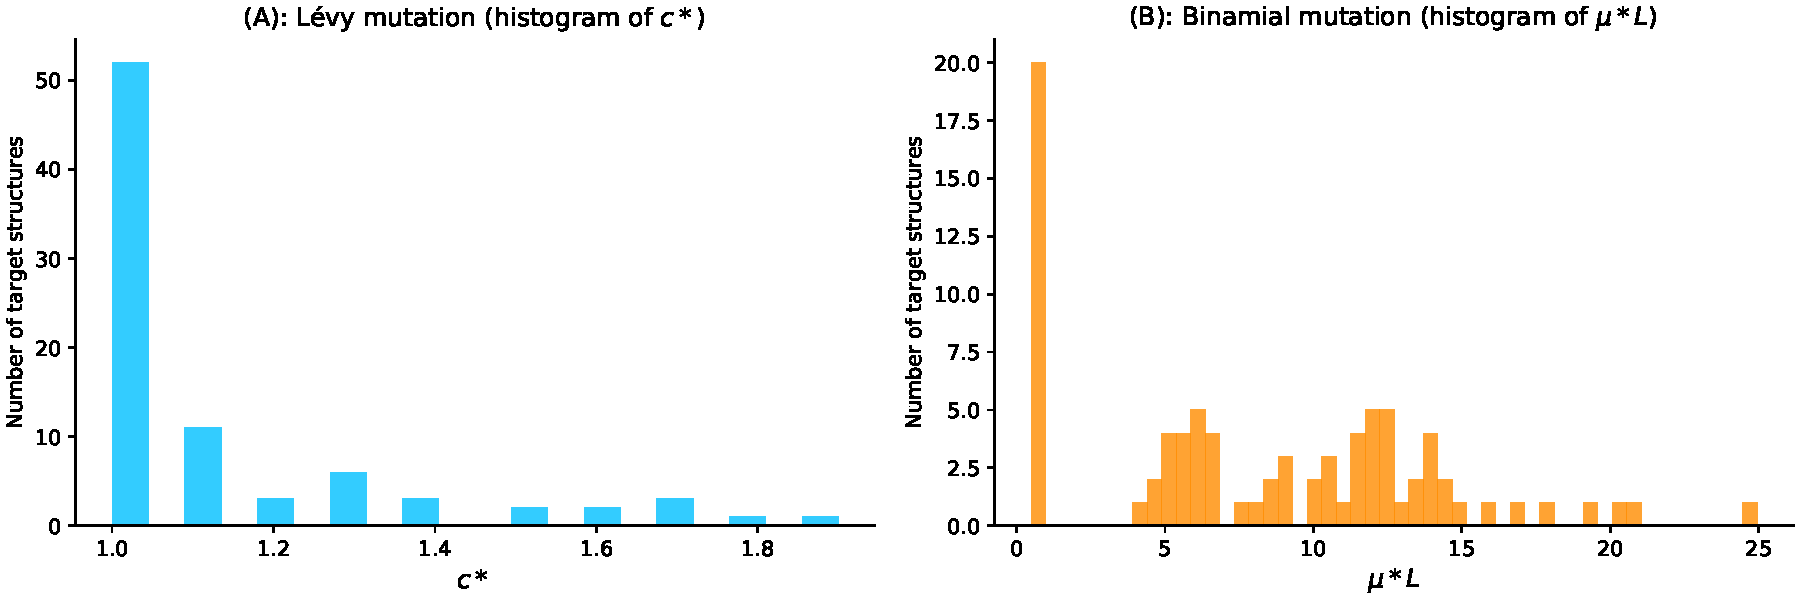
\includegraphics[width=1.0 \linewidth]{../res/images/arnaque/fig3.pdf}
	\caption{Parameter tuning for both binomial and Lévy mutation schemes. (A) Lévy mutation parameter tuning. Histogram of best exponent parameter ($c^*$) for a set of $81$ target structures with different pseudoknot patterns and various lengths. The most frequent best exponent value is $1$. (B) Binomial parameter tuning. Histogram of best mutation rate ($\mu^*$) for the same set of $81$ target structures with different pseudoknots and various lengths. The most frequent best parameter is the low mutation rate ($\approx 1/L$). For some structures, the best mutation rate is the high one for different lengths as well.} \label{Fig:tunning}
\end{figure*}
\section{Experimental results}
We first compared the performance of \texttt{aRNAque} using Lévy mutations to the previous version with local mutations. Secondly, we compared \texttt{aRNAque} to the existing pseudoknotted RNA inverse folding tool \texttt{antaRNA} using two folding tools: \texttt{HotKnots} and \texttt{IPknot}. Finally, we compared the performance of \texttt{aRNAque} (Lévy mutation) to the one of Ivry et al. on a tripod RNA secondary structure.

\subsection{Analysing the best mutation parameter on \texttt{PseudoBase++}: Levy mutation \emph{vs.} local mutation}
The advantage of using a Lévy mutation is its capacity to allow simultaneous search at all scales over the landscape. The search at different scale is often dictated by the exponent parameter of the heavy-tailed distribution. In this first result section, we analyse for $80$ pseudoknotted target structures and for both mutation schemes the distributions of the best mutation parameters.
\begin{itemize}
	\item Binomial mutation: From Figure \ref{Fig:histomut}B, the critical range was identified to be from $0$ to $0.2$ and as $\mu$ becomes greater than $0.1$, the success rate decreases and the average number of generations increases. For each of the $80$ target structures with pseudoknots, $20$ sequences were designed for $\mu \in [0,0.2]$ with a step size of $1/L$. Figure \ref{Fig:tunning}B shows the histogram of the best mutation rate found for each target structure. Two main regimes are apparent: one where the best mutation rate is very low mutation rate ($\approx 1/L$) and another where the high mutation rate is optimal.
	
	\item Lévy mutation: From Figure \ref{Fig:histomut}C, the critical range of $c$ was identified to be $[1,2]$. For $c \in [1,2]$ and a step size of $0.1$, an optimum exponent parameter $c^*$ was investigated for all the $80$ target structures. Figure \ref{Fig:tunning}A shows the histogram of $c^*$. Contrary to binomial mutation, the optimum exponent parameter does not vary too much ($\forall \sigma$, $c^*\approx 1$).
\end{itemize}
Figure \ref{Fig:tunning} shows that when using a Lévy mutation, the optimal mutation rate is the same for most target structures. In contrast, the optimum binomial mutation rate parameter $\mu^*$ mostly varies with different targets. Although both mutation schemes (for the best mutation parameters) have approximately the same success rates, the Lévy flight mutation scheme is more robust to different targets. %Moreover, the median number of generations for the Lévy mutation is lower ($54$ for the Lévy and $92$ for the binomial mutation mode), thus enhancing efficiency.}

\begin{figure}[H]
	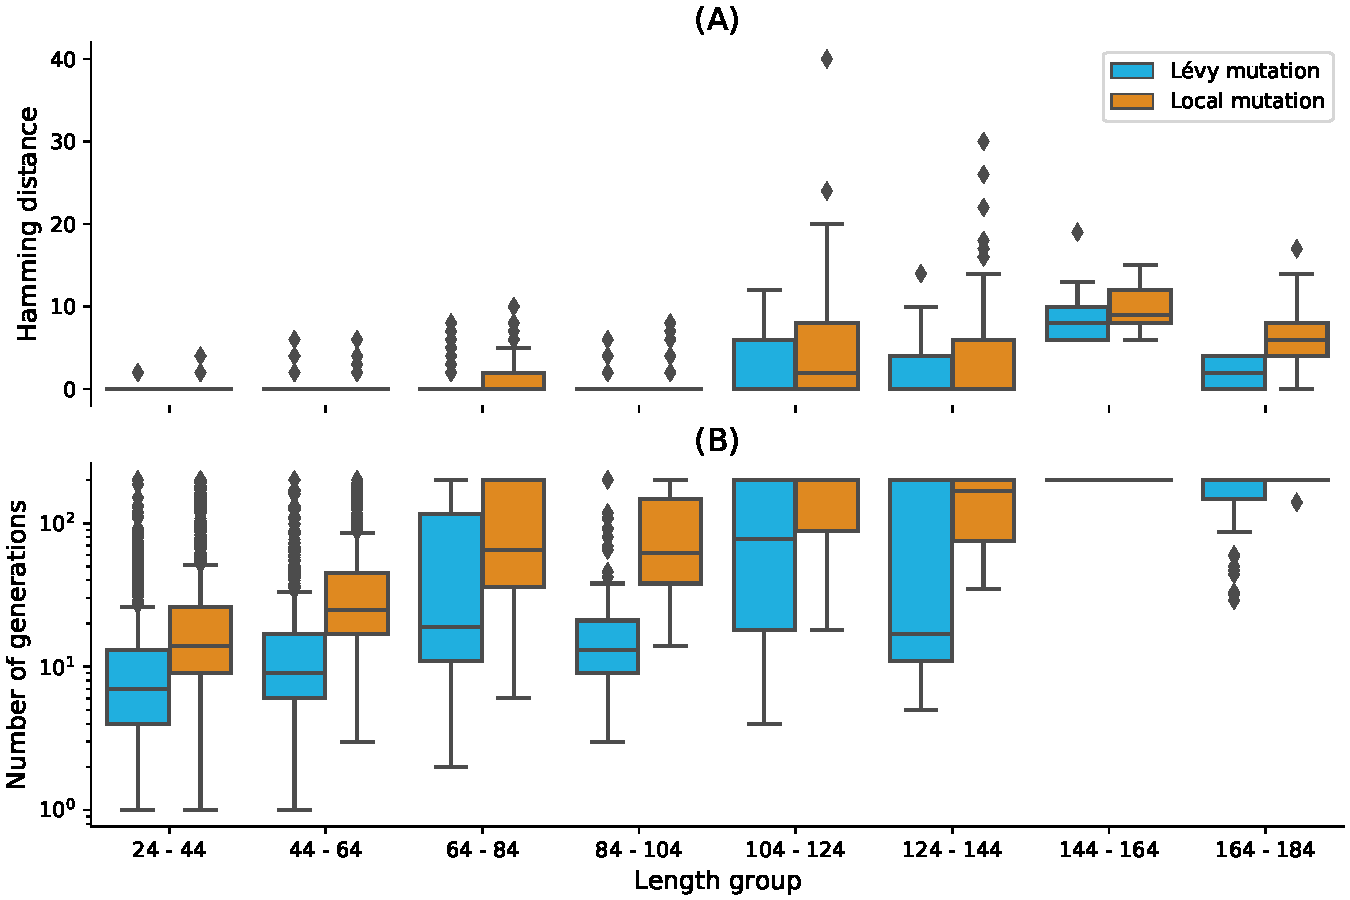
\includegraphics[width=1.0 \linewidth]{../res/images/arnaque/fig4.pdf}
	\small \caption{Lévy mutation mode \emph{vs} local mutation (one-point mutation). (A) Hamming distance distributions \emph{vs.} target structure lengths. (B)  Number of generations distributions for different length groups. In both (A) and (B), lower values indicate better performance. The target structures are solvable in less than $100$ generations for both mutation schemes and most length groups. Still, the difference in the number of generations gets more significant as the target lengths increase, except for the two last length groups for which both mutation schemes mostly failed. The highest difference in terms of median number of generations is $150$ for target lengths in the range $[124-144]$ (respectively $123, 49, 46, 16, 7, 0, 0$ for the length ranges $[84-104], [64-84], [104-124], [44-64], [24-44], [144-164], [164-184]$). Averaging over all length groups, the median number of generations difference between the Levy mutation and the one point mutation is $48$ generations. }\label{Fig:OP_vs_aRNAque}
\end{figure}
\subsection{Performance on \texttt{PseudoBase++}: Levy mutation \emph{vs.} local mutation}
Figure \ref{Fig:OP_vs_aRNAque} shows box plots for the base pair distance (Hamming distance) and the number of generations for increasing target lengths under our two mutation schemes: binomial at low mutation rate (or one point mutation) and the Lévy mutation. For each pseudoknotted RNA target structure in the \texttt{PseudoBase++} dataset, we designed $20$ sequences.  The results show that using the Lévy mutation instead of a local mutation scheme can significantly increase the performance of \texttt{aRNAque}.  The gain was less significant in terms of designed sequences quality  (base pair distance distributions, with a $t$-value $\approx -1.04$ and $p$-value $\approx 0.16$) but more significant in terms of the average number of generations needed for successful matches to target structures (with a $t$-value $\approx -3.6$ and $p$-value $\approx 0.0004$). This result demonstrates a substantial gain in computational time when using a Lévy mutation scheme instead of a purely local mutation.

\subsection{Perfomance on \texttt{non-Eterna100}}
For the first benchmark, we use the \texttt{non-EteRNA} dataset.
Compared to other tools, the statistical results are presented in Table~{\ref{Tab:non-eterna}}.

The results show that our method surpasses~\(8/10\)~of other tools. \(\texttt{ERD}\)~solved~\(2\)~more targets than our method because of its strong decomposition capacity, which allows it to solve the entire~\(\textbf{dataset B}\). With the advantage that our evolutionary algorithm also allows us to fit the nucleotide distribution parameters taken from natural RNA directly in the mutation parameters, we can solve~\(21/24\)~targets from the \(\textbf{dataset B}\). For the~\(\textbf{dataset A}\)~we solve~\(24/29\)~targets which means~\(2\)~more than the previous tools, and for the~\(10\)~last targets we solve~\(7\) targets. Adding all these solved targets together, we obtain a result of~\(52/63\)~as presented in Table~{\ref{Tab:non-eterna}}.
\begin{center}
	\begin{table}[t!]
		\caption{{Summary of performance of \texttt{aRNAque} vs the $10$ other algorithms benchmarked on the non-\texttt{EteRNA100} by Anderson-Lee et al. \cite{anderson2016principles} }} \label{Tab:non-eterna}
		%\vspace{0.5cm}
		%\hspace{2.5cm}
		\centering
		\begin{tabular}[t!]{|c|c|}
			\hline
			\textbf{Methods}& Number of puzzles solved\\
			\hline
			\texttt{SentRNA, NN + full moveset }&$57/63$\\
			\hline
			\texttt{ERD }&$54/63$\\
			\hline
			\texttt{SentRNA, NN + GC pairing }&$53/63$\\
			\hline
			\texttt{SentRNA, NN + All pairing }&$53/63$\\
			\hline
			\texttt{aRNAque}&$\textbf{52/63}$\\
			\hline
			\texttt{RNA-SSD }&$47/63$\\
			\hline
			\texttt{SentRNA, NN only}&$46/63$\\
			\hline
			\texttt{INFO-RNA }&$45/63$\\
			\hline
			\texttt{MODENA }&$32/63$\\
			\hline
			\texttt{NUPACK}&$29/63$\\
			\hline
			\texttt{IncaRNAtion}&$28/63$\\
			\hline
			\texttt{Frnakenstein }&$27/63$\\
			\hline
			\texttt{RNAinverse}&$20/63$\\
			\hline
			\texttt{RNAfbinv}&$0/63$\\
			\hline
		\end{tabular}
	\end{table}
\end{center}
\subsection{Performance on \texttt{PseudoBase++}: \texttt{aRNAque} \emph{vs.} \texttt{antaRNA}}
\subsubsection{General performance analysis using both \texttt{Hotknots} and \texttt{IPknot}}
We also compared the sequences designed using \texttt{aRNAque} (with the Lévy mutation scheme) to those produced by \texttt{antaRNA}. Figures \ref{Fig:antaRNA_vs_aRNAque}A and \ref{Fig:antaRNA_vs_aRNAque}C show the base pair distance distribution for each category of pseudoknotted target structure and the mean of the base pair distance plotted against the length of the target secondary structures. For \texttt{antaRNA}, and when using \texttt{IPknot} as a folding tool, finding sequences that fold into the target becomes increasingly difficult with pseudoknot complexity (median base-pair distance distribution increases). On the other hand, \texttt{aRNAque}’s performance improves as pseudoknot complexity increases (e.g. the mean base-distance decreases with the pseudoknot complexity). 
%In sum, as target length increases, the performance of \texttt{antaRNA} (local search) is considerably degraded , while \texttt{aRNAque} (Lévy flight search) stays almost constant.

A second benchmark using \texttt{HotKnots} as a folding tool was performed on the same dataset. For both \texttt{aRNAque} and \texttt{antaRNA}, the more complex the pseudoknot motifs, the worse is the tool performance (median of the base-pair distance distribution increases). Figures \ref{Fig:antaRNA_vs_aRNAque}B and \ref{Fig:antaRNA_vs_aRNAque}D show the base pair distance distributions with respect to the pseudoknot motifs for both \texttt{aRNAque} and \texttt{antaRNA}. Even though both performances degrade as target length increases, \texttt{aRNAque} (Lévy flight evolutionary search) performance remains almost constant for all the target lengths greater than $60$.
\begin{figure*}[t!]
	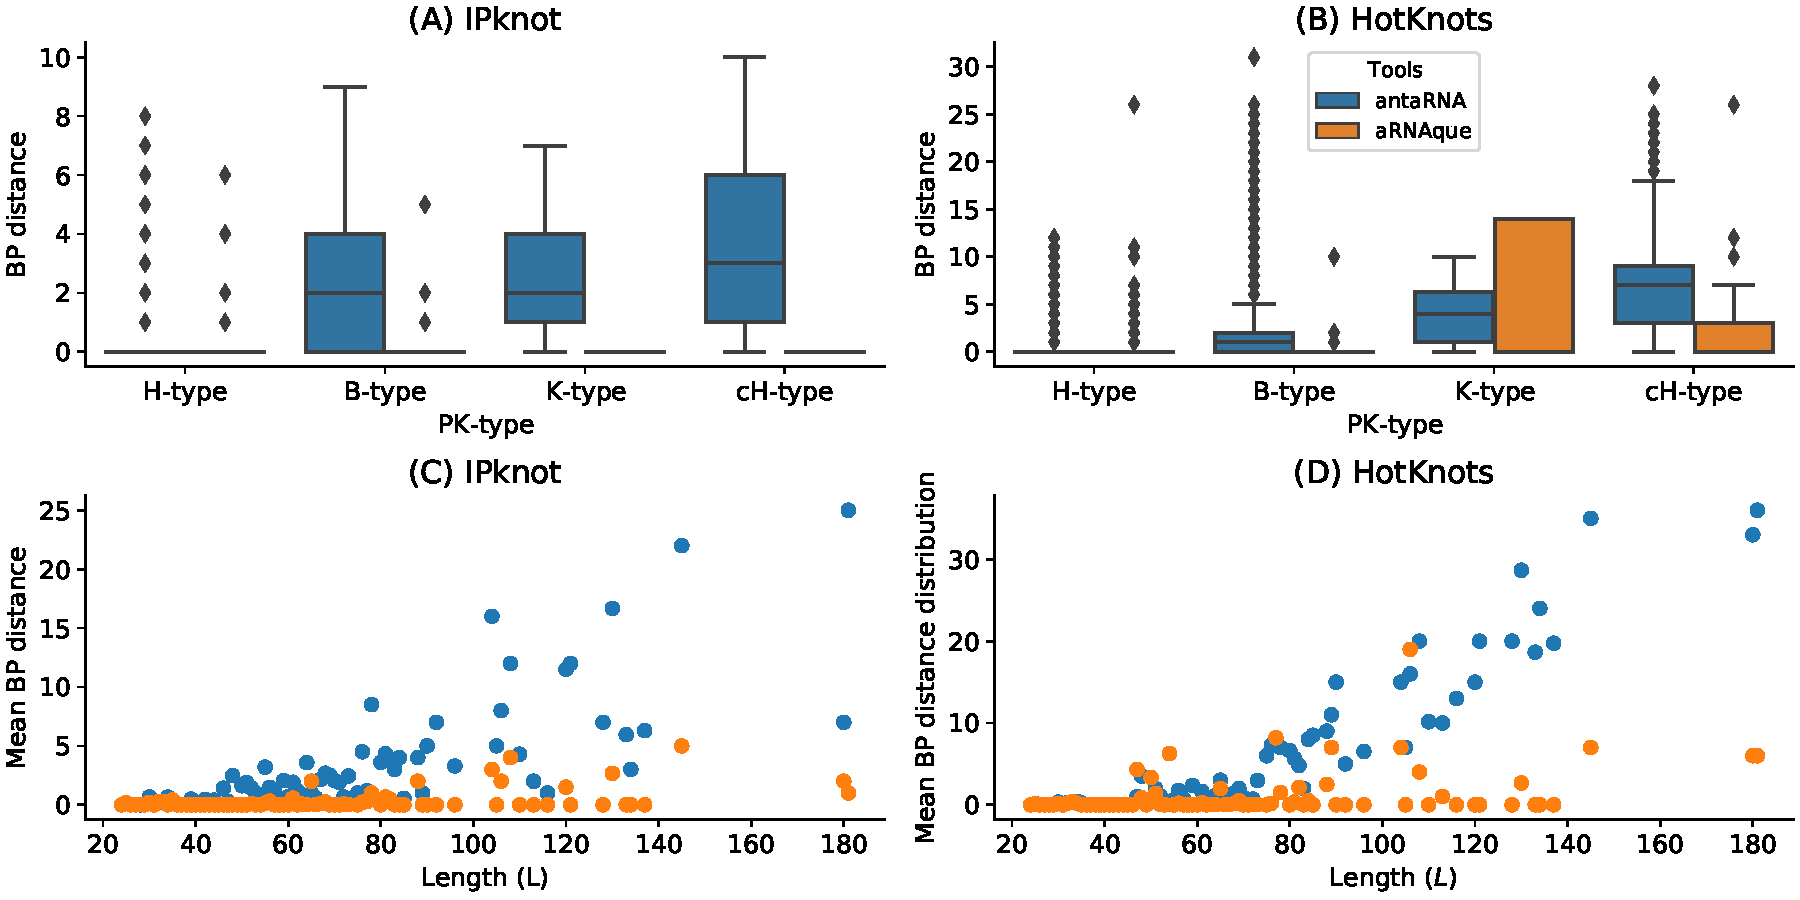
\includegraphics[width=1.0\linewidth]{../res/images/arnaque/fig5.pdf}
	\caption{\texttt{aRNAque} \emph{vs} \texttt{antaRNA} on \texttt{PseudoBase++} dataset using both  \texttt{IPknot} and \texttt{HotKnots}. Lower values imply better performance. (A, B) Base pair distance distributions of the designed sequences to the target structure for different pseudoknot types. (C,D) Mean base pair distance against target lengths. }\label{Fig:antaRNA_vs_aRNAque}
\end{figure*}
\subsubsection{GC--content analysis of the designed sequences using \texttt{IPknot}}
The GC--content of an RNA sequence $S$ measures the concentration of G-C nucleotide in $S$ and influences its stability and biological function. Therefore, the ability of an inverse folding tool to control the GC--content is of vital importance for designing functional RNA sequences. Both \texttt{antaRNA} and \texttt{aRNAque} allow to control the GC--content at different levels of the optimization process: \texttt{aRNAque} through the mutation parameters $P_C$ and $P_N$; \texttt{antaRNA} with the parameter $tGC\in [ 0,1 ]$. In this section, we compare the performance of each tool for fixed GC--content values and analyse each tool's ability to control the GC--content. For each pseudoknotted target structure in the \texttt{PseudoBase++} dataset, four different GC-content values $\{0.25,0.5, 0.75, 1\}$, a poll of $20$ sequences is designed using \texttt{IPknot} as folding tool. That results in $5320$ designed sequences for each GC-content value and tool. The number of successes is the total number of sequences that fold exactly into the given target structure (i.e. the designed sequence folds into a structure at base-pair distance $0$ from the target structure). Figure \ref{Fig:GC_content} shows respectively the base pair distance distributions, the GC distance distributions and the number of successes for both \texttt{aRNAque} and \texttt{antaRNA}. The results show that the performance (in terms of success number) varies considerably with the GC--content values for both tools, and the best performance is obtained for both tools with a GC--content value of $0.5$. When comparing the GC-content distance (i.e absolute value of the difference between the targeted GC--content and the actual GC--content values of the designed sequences) distributions, both GC--content distance median distributions increase, whereas \texttt{antaRNA} controls significantly better the GC-content (See Figure \ref{Fig:GC_content}B). On average, for the respective GC-content values $\{0.25, 0.5, 0.75, 1\}$, \texttt{antaRNA}'s sequences have respectively $0.2569, 0.4952, 0.7314, 0.8684$ whereas  \texttt{aRNAque}'s sequences have respectively $0.3649, 0.4910,$ $ 0.6231, 0.811$; the main difference is at fixed GC-content values $0.25$ and $0.75$. Even though \texttt{antaRNA} designs sequences with better control of the GC-content, the gap in success rate still remains remarkable compared to \texttt{aRNAque}(See Figure \ref{Fig:GC_content}A and Figure \ref{Fig:GC_content}C).
\begin{figure*}[t!]
	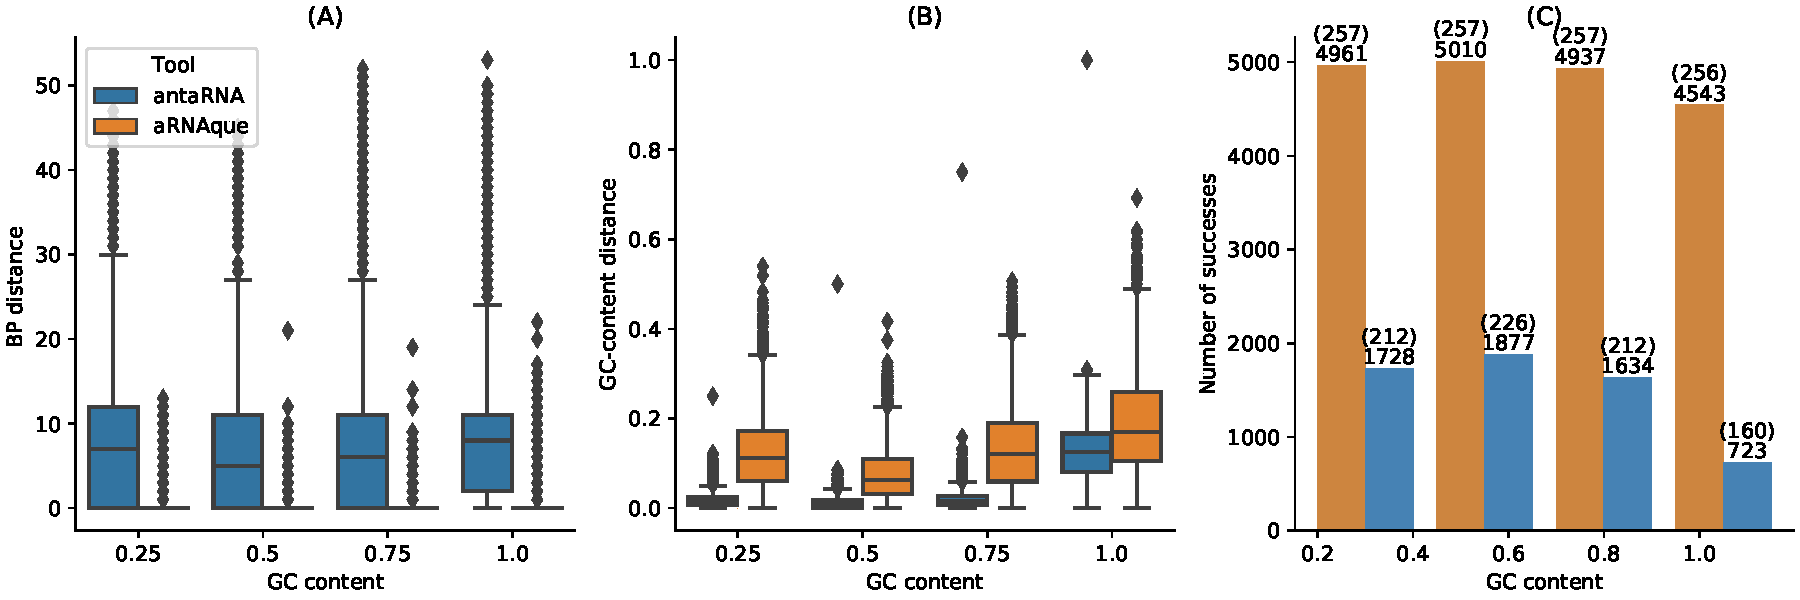
\includegraphics[width=1.0\linewidth]{../res/images/arnaque/fig6.pdf}
	\caption{\texttt{aRNAque} \emph{vs} \texttt{antaRNA} on \texttt{PseudoBase++} dataset using \texttt{IPknot}: GC--content analysis. (A) Base-pair distance ditributions. (B) GC--content distance distributions. The difference betwen the targeted GC-content and the actual GC-content values. In (A,B), lower values imply better performance. (C) Number of successes realised by both inverse folding tools. Two values are considered: the up value represent the number targets successfully solved for each GC-content value out of the $266$ targets benchmarked; the down values represent the number sequences folding into the targeted secondary structure.}\label{Fig:GC_content}
\end{figure*}
\subsubsection{Diversity of the designed sequences}
Another advantage of using a Levy mutation when designing RNA sequences is to increase the chance of designing sequences with high diversity. Here, we use the positional entropy of each pool of $20$ sequences previously designed for each pseudoknotted target structure to compare the diversity of RNA of both tools \texttt{antaRNA} and \texttt{aRNAque} (Lévy search). We also compare it to the diversity of the designed sequences using the old version of \texttt{aRNAque} (Local search). The results show that the sequence diversity of both \texttt{antaRNA} and \texttt{aRNAque} (Lévy search) varies with the GC--content values, where the more diversified pool of sequence is achieved with a GC--content value of $0.5$. When comparing the pool of designed sequences with highest entropy (i.e. with a fixed GC-content of $0.5$) to the one of the old version of \texttt{aRNAque} (Local search), the \texttt{aRNAque} (Lévy search) and \texttt{antaRNA} produce sequences with similar entropy (i.e. with a median entropy of $61.01$ for Lévy search respectively $59.65$ for \texttt{antaRNA} (see Figure \ref{Fig:result_diversity}), whereas the entropy of the sequences designed using the Local search is lower. For the three others fixed GC-content values (i.e. $\{0.25, 0.75, 1 \}$, \texttt{aRNAque} (Lévy search) produces sequences with the highest entropy (respectively a median entropy of $58.9, 60.08, 51.52$ against  $53.42, 54.63, 48.38$ for \texttt{antaRNA}).
%In summary, the updated version of \texttt{aRNAque} (Lévy search) allows designing RNA sequences of high diversity with . 
\begin{figure*}[ht]
	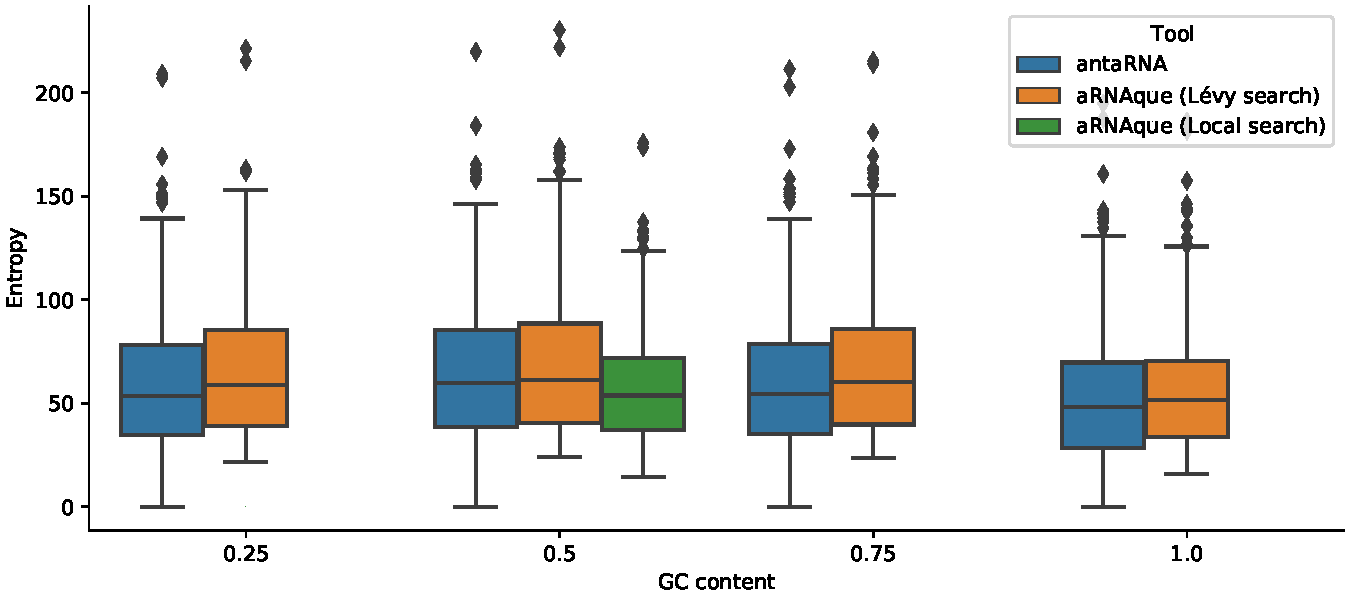
\includegraphics[width=1.0\linewidth]{../res/images/arnaque/fig7.pdf}
	\caption{\texttt{aRNAque} \emph{vs} \texttt{antaRNA} on \texttt{PseudoBase++} dataset using \texttt{IPknot}: Diversity analysis. The positional entropy distributions plotted agains the targeted GC--content values.  Higher values imply better performance.}\label{Fig:result_diversity}
\end{figure*}
\subsection{Performance on \texttt{Eterna100} dataset}

We performed a third benchmark on the \texttt{Eterna100} datasets. First, on the \texttt{Eterna100-V1} dataset, the Lévy flight version of \texttt{aRNAque} successfully designed $89\%$ of the targets and the one-point mutation (local mutation) version achieved $91\%$ of success, suggesting that for some target structures, local mutation can outperform the Lévy mutation scheme. Combining the two solutions, \texttt{aRNAque} solved in total $92\%$ of the targets of \texttt{Eterna100-V1} (see also \cite{merleau2021simple}). 

When analysing the performance of Lévy flight for low and high base pair densities separately, the median number of generations of high base pair density targets was lower than the one with low base-pair density ($8$ generations for high density and $18$ for the low base pairs density targets). The same observation was drawn for the success rate. For the low base-pair density targets, the Lévy flight achieved $87\%$ ($49/56$) success whereas, for the high base-pair density, it achieved $91\%$ ($40/44$). The same analysis can be done when comparing the one-point mutation results for the high-density targets to the Lévy flight mutation. The median number of generations for the low-density targets when using a one-point mutation operator was $34$ (respectively $24$ for the high base pair density targets) (see Figure \ref{Fig:diversity2}A). 


A new benchmark was performed on \texttt{Eterna100-V2} with \texttt{aRNAque} achieving a $93\%$ success rate when combining the designed solutions for both mutation schemes. Compared to recently reported benchmark results \cite{Eterna}, \texttt{aRNAque} achieved similar performance to \texttt{NEMO} on \texttt{Eterna-V2}: one target was unsolved by all existing tools and one target solved only by \texttt{NEMO} remained unsolved by \texttt{aRNAque}. 
\begin{figure*}[t!]
	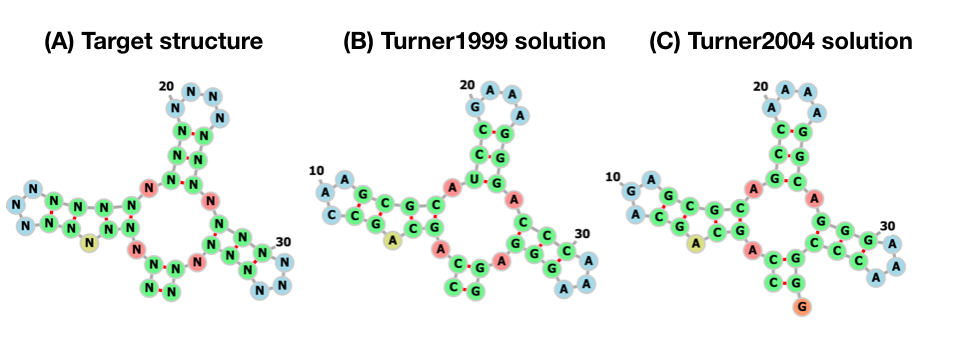
\includegraphics[width=1.0\linewidth]{../res/images/arnaque/fig9.png}
	\caption{\texttt{aRNAque}'s performance on a TRIPOD secondary structure. (A) The tripod target structure. (B) \texttt{aRNAque}'s solution using the Turner1999 energy parameter sets. (C) \texttt{aRNAque}'s solution using the Turner2004 energy parameter sets.}
	\label{Fig:tripod}
\end{figure*}
\subsection{\texttt{aRNAque} performance on a tripod secondary structure}

Finally, we performed a benchmark on a tripod target secondary structure. The tripod secondary structure was used as a third test case in the work of Ivry et al. \cite{ivry2009image}, and it does not contain any pseudoknot interactions. It comprises four stems, three of which with terminal hairpins, surrounding a multibranch loop (See Figure \ref{Fig:tripod}A). The tripod target structure was proved to be very challenging, especially because of its multiloop component, which is also found in some of the unsolved \texttt{Eterna100} target structures. We perform here, for both energy parameters \texttt{Turner1999} and  \texttt{Turner2004}, $100$ independent designs, using a population size of $100$ RNA sequences and a maximum of $5000$ generations. The mutation parameters used are: $P_C=\{0.4,0.5,0.1,0,0,0\}$, $P_N=\{0.7,0.1,0.1,0.1\}$ and $c=1.5$. When using the \texttt{Turner2004} energy parameter set, none of the $100$ designed RNA sequences was successful (i.e, $0$ sequence folds exactly into the target structure after $5000$ generations). Figure \ref{Fig:tripod}B shows one of the best solutions obtained out of $100$ designed sequences when using the \texttt{Turner2004}, the designed sequence folds into a structure at one error base-pair distance from the target structure. In contrast, when using the \texttt{Turner1999} energy parameters, we successfully designed the tripod secondary structure (See Figure \ref{Fig:tripod}C). The $100$ sequences designed folded exactly into the target structure with an average median number of generations $20$. When comparing both solutions to the one obtained in \cite{ivry2009image}, \texttt{aRNAque} (with no need of changing the RNA structure distance) can successfully design the multibranch loop component with one base pair error using the \texttt{Turner2004} energy parameter whereas \texttt{RNAinverse} (with the DoPloCompare distance) failed to design the multibranch loop, and the solution was at $2$ base-pair distance error.

\begin{figure}[t!]
	\begin{center}
		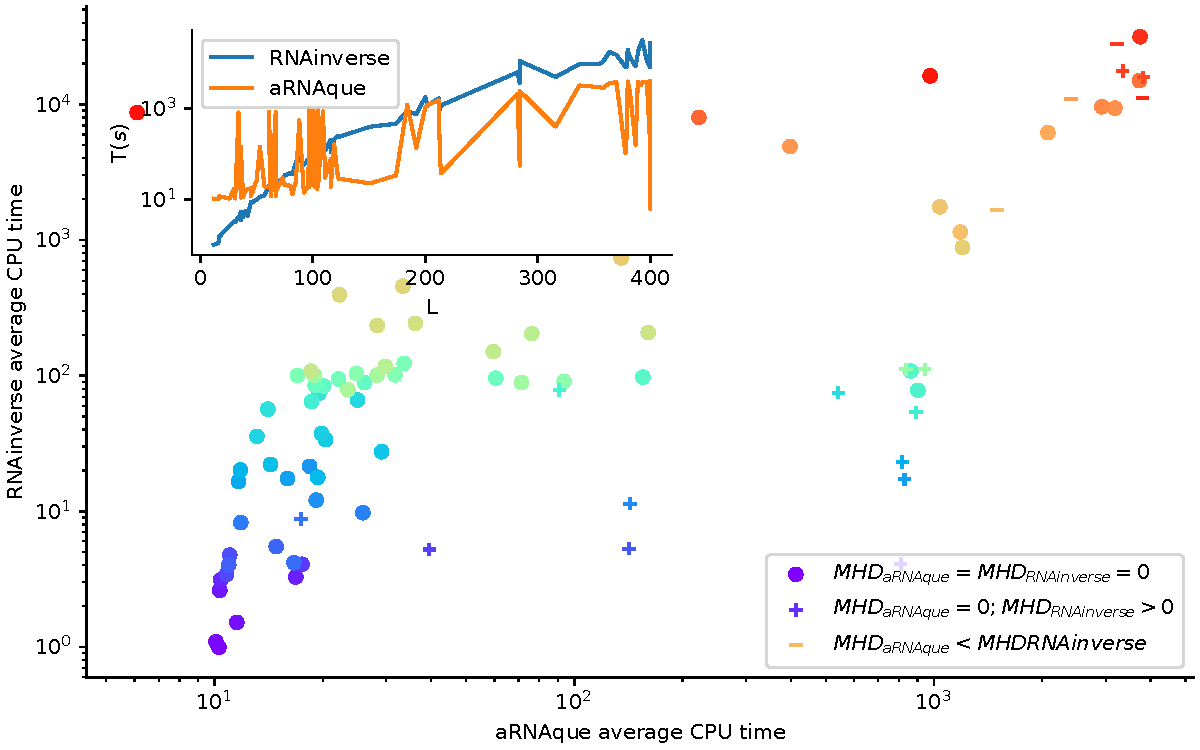
\includegraphics[width=0.98\columnwidth]{../res/images/arnaque/cpuvssuccess.pdf}
		\caption{{CPU time: \texttt{RNAinverse} $vs.$ \texttt{aRNAque}. Each bubble corresponds to a target structure in \texttt{EteRNA100} dataset and, their colours are proportional to the length of the targets. In the legend, MHD stands for Median Hamming distance, and the different markers represent---('o') $100\%$ success for both tools---('+') $100\%$ success for \texttt{aRNAque} and not for \texttt{RNAinverse}---('-') for the case both tools fail to find at least one sequence that folds into the target. Underlying the CPU time difference is the inside plot that shows the CPU time (in seconds) as a target length function.}}
		\label{719148}
	\end{center}
\end{figure}
\subsection{Complexity and CPU time comparison}
{\label{101705}}

An evolutionary algorithm's complexity is often considered to be the number of fitness evaluations needed to solve a given problem. That complexity depends on the number of generations and the population size parameters. For our evolutionary algorithm, we have three objective functions. Therefore, in the worst case the number of evaluation needed is:~ \[f\left(T,t,N\right)=\left(2T+t\right)\times N\]
Where \(T\) is the number of generation need to get at least one sequence that folds into the target and \(t\) the number of generations for performing the ensemble defect refinement.~

\subsubsection{Accuracy and speed comparisons on the \(\textbf{dataset A}\)}
{\label{114736}}

After benchmarking our algorithm on existing datasets and comparing the results obtained to previous tools, we also deemed it is important to address our methods' accuracy and speed comparisons. Here we present time and accuracy comparison on \(\textbf{dataset A}\). The formula used to compute \(E_{t}(s)\) is the same used in \cite{esmaili2015erd} and it is given by:
\begin{equation} 
E_{t}(s)=\frac{\text{Total Execution Time}}{Sc}\nonumber \\
\end{equation}

In Table~{\ref{Tab5:speedandaccuracy}}, our results are compared to the benchmark performed in \cite{esmaili2015erd} and the best results are indicated in bold. As we can see, \texttt{aRNAque} solves \(2\) targets (\(\textbf{RF00009}\) and~\(\textbf{RF00028}\)) previously unsolved by~\(\texttt{INFO-RNA}\) and~\(\texttt{MODENA}\), and~\(2\) other targets unsolved by \(\texttt{ERD}\) (~\(\textbf{RF00030}\)
and~\(\textbf{RF00018}\)). This result allows our algorithm to obtain the best accuracy over all other existing algorithms found in the literature. We can notice that even though for a very few cases we have gotten better speed, the computational time is much more expensive than \(\texttt{ERD}\) and \(\texttt{INFO-RNA}\). This can be understood by the fact that when we use a selection function different from the fitness function, we evaluate every sequence twice at each generation, which consequently increases our algorithm's computation time.
%\onecolumn

\subsubsection{CPU time comparison: \(\texttt{RNAinverse}\) vs.
	\(\texttt{aRNAque}\) on \texttt{EteRNA100}. } 

{\label{391327}}

Since our previous benchmarks on~\(\texttt{EteRNA100}\) using the Turner2004 energy's parameters reveal that \texttt{RNAinverse}, one of the oldest inverse folding tools, stands behind \texttt{aRNAque} solving $66\%$ of the dataset; we also compare its computational time to our implementation.
Figure~{\ref{719148}}~shows the CPU time in seconds needed to design for each target in the~\(\texttt{EteRNA100}\),~\(5\) sequences. As the \(\texttt{RNAinverse}\) time increases exponentially with the length of the target, the \(\texttt{aRNAque}\) one does not. 


\section{Conclusion and discussion}
We investigated an evolutionary approach to improve the existing solutions to the RNA inverse folding problem in this work. As a result, we proposed a new EA \texttt{python} tool called \texttt{aRNAque}.  \texttt{aRNAque} implements a Lévy flight mutation scheme and supports pseudoknottted RNA secondary structures. The benefit of a Lévy flight over a purely local (binomial with $\mu<<1$ or a single point mutation) mutation search allowed us to explore RNA sequence space at all scales. Such a heavy tailed distribution in the number of point mutations permitted the design of more diversified sequences and reduced the number of evaluations of the evolutionary algorithm implemented in \texttt{aRNAque}. The main advantage of using a Lévy flight over local search is a reduction in the number of generations required to reach a target. This is because the infrequent occurrence of a high number of mutations allow a diverse set of sequences among early generations, without the loss of robust local search. One consequence is a rapid increase in the population mean fitness over time and a rapid convergence to the target of the maximally fit sequence. To illustrate that advantage, we ran \texttt{aRNAque} starting from an initial population of unfolded sequences both for a "one point mutation" and "Lévy mutation".

Figures  \ref{Fig:diversity}C and  \ref{Fig:diversity}D show respectively the max/mean fitness over time and the number of distinct structures discovered over time plotted against the number of distinct sequences. When using a Lévy mutation scheme, the mean fitness increases faster in the beginning but stays lower than the one using local mutations. Later in the optimisation, a big jump or high mutation on the RNA sequences produces structures with fewer similarities and, by consequence, worse fitness. In the $(5-10)^{th}$ generation, sequences folding into the target are already present in the Lévy flight population, but only at the $30^{th}$ generation are similar sequences present in the local search population. The Lévy flight also allows exploration of both the structure and sequence spaces, providing a higher diversity of structures for any given set of sequences (Figure \ref{Fig:diversity}D). Using the mean entropy of structures as an alternate measure of diversity, we see in Figure \ref{Fig:diversity}A how a Lévy flight achieves high diversity early in implementation, and maintains a higher diversity over all generations than a local search algorithm. Although the mutation parameters $P_C$ and $P_N$ influence the absolute diversity of the designed sequences, the Lévy flight always tends to achieve a higher relative diversity than local search, all else being equal. 

\begin{figure}[t!]
	\centering
	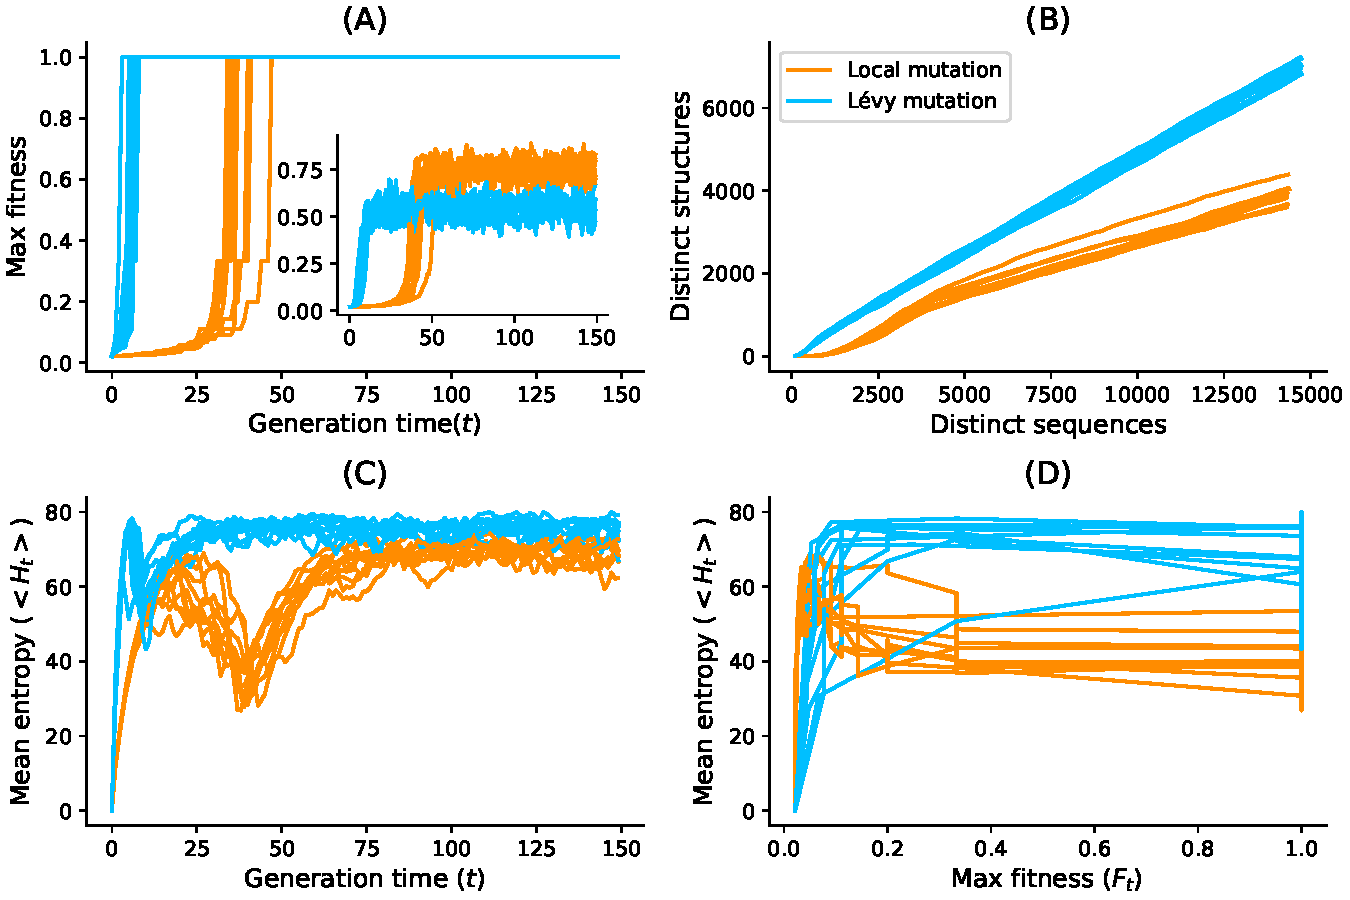
\includegraphics[width=1.0\linewidth]{../res/images/arnaque/fig8.pdf}
	\small 
	\caption{Lévy mutation \emph{vs} one-point mutation: diversity analysis. For the \texttt{Eterna100} target structure \textit{[CloudBeta] 5 Adjacent Stack Multi-Branch Loop}, ten independent runs were performed in which a minimum of $10$ sequences were designed per run.  (A) Max fitness and mean fitness (inset) over time. (B) Distinct sequences \emph{vs.} Distinct structures over time. (C) Mean Shannon entropy of the population sequences over time for both binomial and Lévy mutation. (D) The max fitness plotted against the entropy over time.}
	\label{Fig:diversity}
	
\end{figure}

We argue that the improved performance of the Lévy Flight over local search in target RNA structures is due to the high base pair density of pseudoknotted structures. Given that pseudoknots present a high density of interactions, there are dramatic increases in possible incorrect folds and thus becoming trapped near local optima \cite{hajdin2013accurate}. Large numbers of mutations in paired positions, as implied by a heavy tailed distribution, are necessary to explore radically different solutions. 

To illustrate that Lévy Flight performance was due to base pair density, we clustered the benchmark datasets into two classes: one cluster for target structures with low base pair density (density $\leq 0.5$) and a second cluster for structures with high base pair density (density $> 0.5$). Figure \ref{Fig:diversity2}B shows the number of target sequences available in each low and high density category. The number of targets available in each category are colored according to the percentage of pseudoknot-free targets (\texttt{Eterna100-V1}) vs. targets with pseudoknots (\texttt{Pseudobase++}), showing that pseudoknots are strongly associated with high base pair densities: $71\%$ of the pseudoknotted target structures have a high base pair density.  In contrast, the \texttt{Eterna100} dataset without psuedoknots has somewhat higher representation at low base pair density. If it is true that improved Lévy Flight performance is indeed tied to base pair density, it is possible that similar heavy-tailed mutation schemes could offer a scalable solution to even more complex inverse folding problems. 
\begin{figure}[t!]
	\centering
	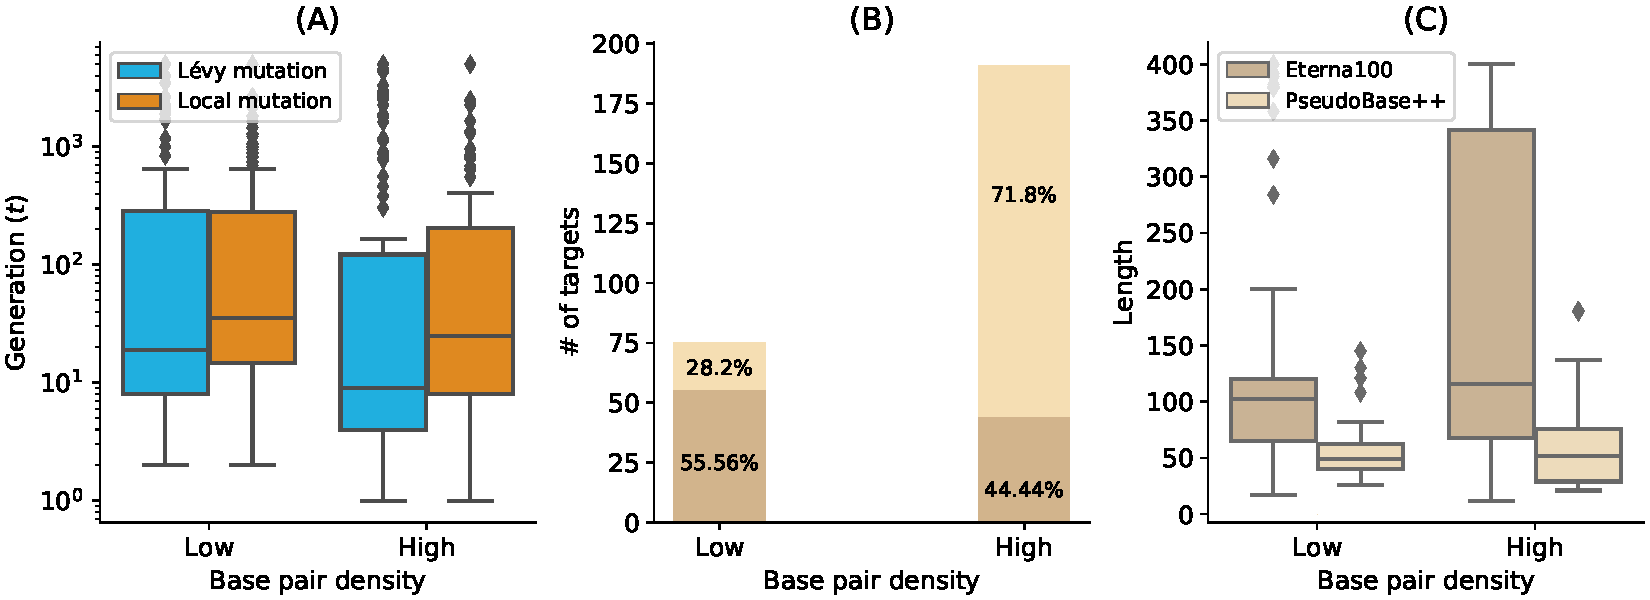
\includegraphics[width=1.05\linewidth]{../res/images/arnaque/fig10.pdf}
	\small
	\caption{Lévy mutation \emph{vs.} Local mutation: performance analysis with respect to the base-pair density. The higher the base-pair density is, the more useful the Lévy mutation scheme to speed up the optimization EA. (A) Distributions of number of generations for the low and high base-pair density targets of the \texttt{Eterna100} dataset. (B) Percentages of targets with low and high base-pair density for the \texttt{Eterna100} and \texttt{PseudBase++}. (C) The length distributions of the low and high base-pair density pseudoknot-free and pseudoknotted targets.} \label{Fig:diversity2}
\end{figure}
Although we believe that Lévy flight-type search algorithms offer a valuable alternative to local search, we emphasise that its enhanced performance over say \texttt{antaRNA} is partially influenced by the specific capabilities of existing folding tools. Their limitations may account for the degradation of these tools as the pseudoknot motifs get increasingly complex. Another possible limitation is that most pseudoknotted and pseudoknot-free target structures are relatively easy to solve (in less than $100$ generation time), requiring more investigations for the unsolved targets to illustrate the performance of the Lévy mutation better.

Our results show general and significant improvements in the design of RNA secondary structures compared to the standard evolutionary algorithm mutation scheme with a mutation parameter $\approx 1/L$, where $L$ is the sequence solution length. Not only does Lévy flight mutations lead to greater diversity of RNA sequence solutions, but it also reduces the evolutionary algorithm’s number of evaluations, thus improving computing time. 

%\include{multiToC} % <--- just debug stuff, ignore for your documents
% ********************************************************************
\part{Discussion and Perspectives}
%************************************************
\chapter{RAFFT and continuous transition in evolution}\label{ch:continuity}


% Backmatter
%*******************************************************
\appendix
%\renewcommand{\thechapter}{\alph{chapter}}
\cleardoublepage
\part{Appendix}
%********************************************************************
% Appendix
%*******************************************************
% If problems with the headers: get headings in appendix etc. right
%\markboth{\spacedlowsmallcaps{Appendix}}{\spacedlowsmallcaps{Appendix}}
\chapter{Appendix Test}
Lorem ipsum at nusquam appellantur his, ut eos erant homero
concludaturque. Albucius appellantur deterruisset id eam, vivendum
partiendo dissentiet ei ius. Vis melius facilisis ea, sea id convenire
referrentur, takimata adolescens ex duo. Ei harum argumentum per. Eam
vidit exerci appetere ad, ut vel zzril intellegam interpretaris.
\graffito{More dummy text.}

%Errem omnium ea per, pro congue populo ornatus cu, ex qui dicant
%nemore melius. No pri diam iriure euismod. Graecis eleifend
%appellantur quo id. Id corpora inimicus nam, facer nonummy ne pro,
%kasd repudiandae ei mei. Mea menandri mediocrem dissentiet cu, ex
%nominati imperdiet nec, sea odio duis vocent ei. Tempor everti
%appareat cu ius, ridens audiam an qui, aliquid admodum conceptam ne
%qui. Vis ea melius nostrum, mel alienum euripidis eu.

\section{Appendix Section Test}
Test: \autoref{tab:moreexample} (This reference should have a
lowercase, small caps \spacedlowsmallcaps{A} if the option
\texttt{floatperchapter} is activated, just as in the table itself
 $\rightarrow$ however, this does not work at the moment.)

\begin{table}[h]
    \myfloatalign
    \begin{tabularx}{\textwidth}{Xll} \toprule
        \tableheadline{labitur bonorum pri no} & \tableheadline{que vista}
        & \tableheadline{human} \\ \midrule
        fastidii ea ius & germano &  demonstratea \\
        suscipit instructior & titulo & personas \\
        %postulant quo & westeuropee & sanctificatec \\
        \midrule
        quaestio philosophia & facto & demonstrated \\
        %autem vulputate ex & parola & romanic \\
        %usu mucius iisque & studio & sanctificatef \\
        \bottomrule
    \end{tabularx}
    \caption[Autem usu id]{Autem usu id.}
    \label{tab:moreexample}
\end{table}

%Nulla fastidii ea ius, exerci suscipit instructior te nam, in ullum
%postulant quo. Congue quaestio philosophia his at, sea odio autem
%vulputate ex. Cu usu mucius iisque voluptua. Sit maiorum propriae at,
%ea cum primis intellegat. Hinc cotidieque reprehendunt eu nec. Autem
%timeam deleniti usu id, in nec nibh altera.




\section{Another Appendix Section Test}
Equidem detraxit cu nam, vix eu delenit periculis. Eos ut vero
constituto, no vidit propriae complectitur sea. Diceret nonummy in
has, no qui eligendi recteque consetetur. Mel eu dictas suscipiantur,
et sed placerat oporteat. At ipsum electram mei, ad aeque atomorum
mea. There is also a useless Pascal listing below: \autoref{lst:useless}.

\begin{lstlisting}[float=b,language=Pascal,frame=tb,caption={A floating example (\texttt{listings} manual)},label=lst:useless]
for i:=maxint downto 0 do
begin
{ do nothing }
end;
\end{lstlisting}

%Ei solet nemore consectetuer nam. Ad eam porro impetus, te choro omnes
%evertitur mel. Molestie conclusionemque vel at, no qui omittam
%expetenda efficiendi. Eu quo nobis offendit, verterem scriptorem ne
%vix.


%********************************************************************
% Other Stuff in the Back
%*******************************************************
\cleardoublepage%********************************************************************
% Bibliography
%*******************************************************
% work-around to have small caps also here in the headline
% https://tex.stackexchange.com/questions/188126/wrong-header-in-bibliography-classicthesis
% Thanks to Enrico Gregorio
\defbibheading{bibintoc}[\bibname]{%
  \phantomsection
  \manualmark
  \markboth{\spacedlowsmallcaps{#1}}{\spacedlowsmallcaps{#1}}%
  \addtocontents{toc}{\protect\vspace{\beforebibskip}}%
  \addcontentsline{toc}{chapter}{\tocEntry{#1}}%
  \chapter*{#1}%
}
%\bibliographystyle{unsrt}
\printbibliography[heading=bibintoc]


% Old version, will be removed later
% work-around to have small caps also here in the headline
%\manualmark
%\markboth{\spacedlowsmallcaps{\bibname}}{\spacedlowsmallcaps{\bibname}} % work-around to have small caps also
%\phantomsection
%\refstepcounter{dummy}
%\addtocontents{toc}{\protect\vspace{\beforebibskip}} % to have the bib a bit from the rest in the toc
%\addcontentsline{toc}{chapter}{\tocEntry{\bibname}}
%\label{app:bibliography}
%\printbibliography

\cleardoublepage%*******************************************************
% Declaration
%*******************************************************
\pdfbookmark[0]{Declaration}{declaration}
\chapter*{Declaration}
\thispagestyle{empty}

\begin{itemize}
	\item Ich erkenne die Promotionsordnung der Fakult\"at f\"ur Mathematik und Informatik der Universit\"at Leipzig vom 2. Mai 2013 in der Fassung der Ersten \"Anderungssatzung vom 16. Oktober 2017 an. \vspace{0.2cm}
	
	\item Die eingereichte Arbeit wurde nicht in gleicher oder \"ahnlicher Form einer anderen Pr\"ufungsbeh\"orde zum Zwecke einer Promotion oder eines anderen Pr\"ufungsverfahrens vorgelegt. \vspace{0.2cm}
	
	\item Es haben keine fr\"uheren erfolglosen Promotionsversuche stattgefunden. 
	\vspace{0.2cm}
	
\end{itemize}

\vspace*{1.5cm}
\begin{flushleft}
	...............................................\\
	(\myName)
\end{flushleft}

%%% Local Variables: 
%%% mode: latex
%%% TeX-master: "dissdocuments"
%%% End: 


\cleardoublepage\pagestyle{empty}

\hfill

\vfill


\pdfbookmark[0]{Colophon}{colophon}
\section*{Colophon}
This document was typeset using the typographical look-and-feel \texttt{classicthesis} developed by Andr\'e Miede and Ivo Pletikosić.
The style was inspired by Robert Bringhurst's seminal book on typography ``\emph{The Elements of Typographic Style}''.
\texttt{classicthesis} is available for both \LaTeX\ and \mLyX:
\begin{center}
\url{https://bitbucket.org/amiede/classicthesis/}
\end{center}
Happy users of \texttt{classicthesis} usually send a real postcard to the author, a collection of postcards received so far is featured here:
\begin{center}
\url{http://postcards.miede.de/}
\end{center}
Thank you very much for your feedback and contribution.

\bigskip

\noindent\finalVersionString

%Hermann Zapf's \emph{Palatino} and \emph{Euler} type faces (Type~1 PostScript fonts \emph{URW
%Palladio L} and \emph{FPL}) are used. The ``typewriter'' text is typeset in \emph{Bera Mono},
%originally developed by Bitstream, Inc. as ``Bitstream Vera''. (Type~1 PostScript fonts were made
%available by Malte Rosenau and
%Ulrich Dirr.)

%\paragraph{note:} The custom size of the textblock was calculated
%using the directions given by Mr. Bringhurst (pages 26--29 and
%175/176). 10~pt Palatino needs  133.21~pt for the string
%``abcdefghijklmnopqrstuvwxyz''. This yields a good line length between
%24--26~pc (288--312~pt). Using a ``\emph{double square textblock}''
%with a 1:2 ratio this results in a textblock of 312:624~pt (which
%includes the headline in this design). A good alternative would be the
%``\emph{golden section textblock}'' with a ratio of 1:1.62, here
%312:505.44~pt. For comparison, \texttt{DIV9} of the \texttt{typearea}
%package results in a line length of 389~pt (32.4~pc), which is by far
%too long. However, this information will only be of interest for
%hardcore pseudo-typographers like me.%
%
%To make your own calculations, use the following commands and look up
%the corresponding lengths in the book:
%\begin{verbatim}
%    \settowidth{\abcd}{abcdefghijklmnopqrstuvwxyz}
%    \the\abcd\ % prints the value of the length
%\end{verbatim}
%Please see the file \texttt{classicthesis.sty} for some precalculated
%values for Palatino and Minion.
%
%    \settowidth{\abcd}{abcdefghijklmnopqrstuvwxyz}
%    \the\abcd\ % prints the value of the length

% ********************************************************************
% Game Over: Restore, Restart, or Quit?
%*******************************************************
\end{document}
% ********************************************************************
